% mnras_template.tex
%
% LaTeX template for creating an MNRAS paper
%
% v3.0 released 14 May 2015
% (version numbers match those of mnras.cls)
%
% Copyright (C) Royal Astronomical Society 2015
% Authors:
% Keith T. Smith (Royal Astronomical Society)

% Change log
%
% v3.0 May 2015
%    Renamed to match the new package name
%    Version number matches mnras.cls
%    A few minor tweaks to wording
% v1.0 September 2013
%    Beta testing only -never publicly released
%    First version: a simple (ish) template for creating an MNRAS paper

%%%%%%%%%%%%%%%%%%%%%%%%%%%%%%%%%%%%%%%%%%%%%%%%%%
% Basic setup. Most papers should leave these options alone.
\documentclass[fleqn,usenatbib]{mnras}

% MNRAS is set in Times font. If you don't have this installed (most LaTeX
% installations will be fine) or prefer the old Computer Modern fonts, comment
% out the following line
% Depending on your LaTeX fonts installation, you might get better results with one of these:
%\usepackage{mathptmx}
%\usepackage{txfonts}
% Use vector fonts, so it zooms properly in on-screen viewing software
% Don't change these lines unless you know what you are doing
\usepackage[T1]{fontenc}
\usepackage[dvipsnames]{xcolor}
\usepackage{sansmath}
\usepackage{mathtools}
% \usepackage{siunix}
% \usepackage{amsmath}
% Allow "Thomas van Noord" and "Simon de Laguarde" and alike to be sorted by "N" and "L" etc. in the bibliography.
% Write the name in the bibliography as "\VAN{Noord}{Van}{van} Noord, Thomas"
\DeclareRobustCommand{\VAN}[3]{#2}
\let\VANthebibliography\thebibliography
\def\thebibliography{\DeclareRobustCommand{\VAN}[3]{##3}\VANthebibliography}

%%%%% AUTHORS -PLACE YOUR OWN PACKAGES HERE %%%%%

% Only include extra packages if you really need them. Common packages are:
\usepackage{graphicx}	% Including figure files
\usepackage{amsmath}	% Advanced maths commands
\usepackage{amssymb}	% Extra maths symbols
\usepackage{xcolor}
% \usepackage{amsmath}
\usepackage{newtxtext,newtxmath}
%%%%%%%%%%%%%%%%%%%%%%%%%%%%%%%%%%%%%%%%%%%%%%%%%%

%%%%% AUTHORS -PLACE YOUR OWN COMMANDS HERE %%%%%

% Please keep new commands to a minimum, and use \newcommand not \def to avoid
% overwriting existing commands. Example:
\newcommand{\civ}{\ion{C}{IV}}	
\newcommand{\nciv}{N_{\civ}} % per cm-squared
\newcommand{\zciv}{z_{\civ}}
\newcommand{\sciv}{\sigma_{\civ}}
\newcommand{\kms}{kms$^{-1}$} % KLC:
                              % \providecommand{\kms}{\ensuremath{\,{\rm km\,s}^{-1}}} means \kms can then be used in mathmode and textmode w/o issue;  I use the "\," to make a small space before units that then keep units w/number (meaning I don't have a space between number and \kms
\newcommand{\zqso}{z_{\textrm{QSO}}}
\newcommand{\mciv}{\mathcal{M}_{\textrm{\civ}}}
\newcommand{\dd}{\textrm{d}}
\newcommand{\Data}{\mathcal{D}}
\newcommand{\model}{\mathcal{M}}
\renewcommand{\doi}[1]{\href{http://dx.doi.org/#1}{doi:#1}}
\newcommand{\arxiv}[1]{\href{http://arxiv.org/#1}{arxiv:#1}}
\definecolor{flatirons}{HTML}{8B2131}
\definecolor{rez}{HTML}{006400}
\def\txr{\textcolor{BrickRed}}
%%%%%%%%%%%%%%%%%%%%%%%%%%%%%%%%%%%%%%%%%%%%%%%%%%


 \newcommand{\mfho}[1]{\textcolor{flatirons}{[\bf MFH: #1]}}
 \newcommand{\spb}[1]{\textcolor{red}{[\bf SPB: #1]}}
 \newcommand{\rmon}[1]{\textcolor{rez}{[\bf RM: #1]}}

%%%%%%%%%%%%%%%%%%% TITLE PAGE %%%%%%%%%%%%%%%%%%%

% Title of the paper, and the short title which is used in the headers.
% Keep the title short and informative.
\title[\civ\ absorbers in SDSS DR12]{\civ\ absorbers in SDSS DR12:
 detection with Gaussian processes}

% The list of authors, and the short list which is used in the headers.
% If you need two or more lines of authors, add an extra line using \newauthor
\author[R.~Monadi et. al.]{
Reza Monadi$^{1}$\thanks{E-mail: reza.monadi@email.ucr.edu (RM)},
Simeon Bird$^{1}$, Ming-Feng Ho$^{1}$, Kathy L.~Cooksey$^{2}$
%Third Author$^{2,3}$
%and Fourth Author$^{3}$
% List of institutions
\\
$^{1}$University of California, Riverside, U.S.A.\\
$^{2}$University of Hawai`i at Hilo, Hilo, U.S.A.}
%$^{3}$Another Department, Different Institution, Street Address, City Postal Code, Country

%% KLC: if opportunity for DOI link, mine 0000-0001-5810-5225 (e.g.,
%% \author[0000-0001-5810-5225]{Kathy L.~Cooksey})

% These dates will be filled out by the publisher
\date{Accepted XXX. Received YYY; in original form ZZZ}

% Enter the current year, for the copyright statements etc.
\pubyear{2021}

% Don't change these lines
\begin{document}
\label{firstpage}
\pagerange{\pageref{firstpage}--\pageref{lastpage}}
\maketitle

% Abstract of the paper % KLC: I find it odd to have these italicized
% sections of an abstract; is this MNRAS style or personal?
\begin{abstract}
  \emph{Aim}:  We assemble the largest \civ\ absorption line catalogue to date,
  leveraging %or utilizing
  machine learning to remove the need for visual inspection. We also provide a probability to classify the reliability of the absorption system within a quasar spectrum.  \\
  \emph{Method}: We  used Gaussian processes to train a quasar
  continuum model to detect \civ~absorbers.
  %% KLC: A lot of first person (“we this” “we that”). And this part
  %% has a lot of prepositional phrases with repetitive -ity/ify words
  %% How about the following for the preceding sentencet:
  %% The algorithm quantifies the reliability of each CIV system
  %% within a given quasar spectrum, via a probability.
  Our training set was a sample of DR7
  spectra that % KLC: "which" precedes phrase that can be excised from
               % sentence and is preceded by comma; "that" precedes
               % phrase crucial to sentence and is not preceded by comma
  were labelled as \civ~free in the previous largest (visually inspected)
  \civ\ absorption catalogue.
  %% KLC: preceding sentence a bit confusing; how about:
  %% Our training set was a subset of DR7 quasar spectra that had no
  %% detectable CIV absorption (``continuum model'') in the previous largest (visually
  %% inspected) \civ\ absorption catalogue.
  We use Bayesian model selection to decide between our continuum
  model and our absorption-line models. % KLC: compound adjective
  Our catalogue provides maximum a posteriori values and credible intervals
  for \civ\ redshift, column density, and Doppler parameter. % $\zqso$, $\nciv$ and $\sciv$. %% KLC: don't introduce notation w/o defining it and since don't use notation in rest of abstract don't need to introduce it; also think \zqso supposed to be \zciv
  \\ % KLC: can just leave a white line and LaTeX will handle it.
  \emph{Results}: Using a hold-out sample of $1301$
spectra from our training set, we validated our pipeline and obtained
an AUC %% KLC define AUC
of 0.86\%.
We find good purity and completeness values, both $\sim 80\%$, when a probability of $\sim95\%$ is used as the threshold.
We obtain similar \civ~redshifts and rest equivalent widths with our pipeline compared to our training set. % KLC: "training set" was used to indicate the CIV-free spectra earlier so no "training set" is muddled. Either clarify earlier or here.
Applying our model % KLC: what is "model" b/c there is "continuum model" and "absorption-line model" so maybe mean "algorithm"?
to 185,425 selected quasar spectra from SDSS DR12, we produce a catalogue
of 113,775 \civ\ doublets with at least 95\% probability. We detected
\civ~absorption $\zciv ~ 1.5$--5, % KLC: need lower bound; en-dash indicates range; and FYI: I prefer \sim to ~; not sure of the precise mathematical implication but \sim indicates a tighter constraint than ~ to me
including $33$ systems at $\zciv > 5$ % KLC: just "higher redshift" unclear
and
$110$ systems with rest equivalent widths greater than 2\,\AA. % KLC: or whatever is the limit that's an even number; don't need to harp on DR7 in abstract
Our catalogue can guide high resolution follow-up observations and may be cross-matched with galaxy catalogues or other absorption catalogues to investigate the properties the circumgalactic medium.
%for info

  %for info

% The broadnarrow-broad structure allows you to communicate with a wider readership
\end{abstract}

% Select between one and six entries from the list of approved keywords.
% Don't make up new ones.
\begin{keywords}
  (galaxies:) quasars: absorption lines -- methods: statistical
\end{keywords}

%%%%%%%%%%%%%%%%%%%%%%%%%%%%%%%%%%%%%%%%%%%%%%%%%%

%%%%%%%%%%%%%%%%% BODY OF PAPER %%%%%%%%%%%%%%%%%%

\section{Introduction}

Metals, elements heavier than helium, are formed in the hearts of
massive stars and recycled into the interstellar medium (ISM) by
supernovae and stellar winds. Ultimately some of these metals are
transported into the circumgalactic medium (CGM) or even intergalactic medium (IGM). % KLC true and might as well introduce the acronym now
Measurements of the abundance of metals in the
Universe over time thus allow us to study the
cycling of baryons through galaxies and, thus, the
formation and evolution of galaxies \citep{cgmPaper, baryonCycle}.

% Why specifically CIV?
Quasar absorption lines enable % KLC: used "allow" just above
us to measure the abundance of elements and their ionization states
within the intergalactic gas.
Particularly useful is the \civ\ $\lambda,\lambda1548,1550$ % KLC: traditional notation
doublet.
This doublet is caused by a strong transition of an abundant metal that
redshifts into optical bands at  $z ~ 1.5$--5.2, with lower redshifts observable in the UV \citep[e.g.,][]{C10,shul2014} and higher in the IR \citep[e.g.,][]{simcoeetal13,ryanweber09,beckeretal09}. % KLC: or whatever are the latest citations from those authors; seems like you brought in the UV to cite me and Shull so continuing the idea of "cite all the movers and shakers you can to appease referee", should include the high-z authors
The rest wavelengths of the \civ\ doublet make it
detectable outside the \ion{H}{1} Ly$\alpha$ forest.
Moreover, \civ\ has an unsaturated doublet
ratio of $2:1$ for $W_{r,1548}:W_{r,1550}$, easing automated
line detection methods \citep{ChurchillBook}.



\civ\ absorption has been extensively studied; here we will provide an abreviated overview, and the interest reader is referred to \citet[][and references therin]{annualreview} for a more comprehensive reivew. % KLC: need to phrase this carefully; the whole bit needs some massaging b/c it really, really reads "just going to cite all the possible referees. Maybe the leading sentence is or includes "\civ\ is a useful resonance line doublet, enabling the study many physical properties of the CGM over cosmic time."
\cite{rauch1996} measured the temperature and kinematics \civ\ absorbers. \cite{barlow1998} and \cite{Ellison2000} % KLC: comma separated; need proper grammar for citations in text mode; for all similar "comma separated" comments below, maybe just figure out how to rephrase to use parenthetical (\citep) citation
studied the metallicity and enrichment history of the CGM using
the \civ/\ion{H}{I} line ratio. The total abundance and evolution of \civ\ was studied by
\cite{songaila2005, odorico2010, simcoe2011, Hasan1, Hasan2}. % KLC: think you have to divide this up into comma-separated \cite{}, \cite{}
\cite{boks2015} studied the ratio of \civ\ to other metal lines to
constrain the ionization state of the IGM. % KLC: introduced earlier now
\cite{cooper2019} used the ratios of different carbon ions to infer the
ionization state of the absorbing gas in the IGM at a redshift where neutral hydrogen absorption is saturated.
The clustering of \civ\ absorbers systems has been measured by
\cite{sargent1988,  petit1994, chen2000, scannapieco2006}. % KLC: comma separated
\rmon{Also,}
\cite{Adel2005, bordoloi2014, rubin2015, burchett2015, burchett2016} % KLC: comma separated
used close quasar-galaxy pairs to connect \civ\ absorbers to galactic halos.
\civ\ absorbers have been observed at $z > 5$, probing the tail end of the reionization epoch by \cite{becker2009, weber2009, odorico2013,codoreanu2018, doughty2023}. % KLC: comma separated
Most relevant to our current work, \cite{C13} detected strong \civ\ absorbers in the low signal-to-noise spectra of the Sloan Digital Sky Survey (SDSS) \citep{sdssdr7, Eisen11}.
On the theory side, \civ\ has been associated with enriched gas surrounding galactic halos in cosmological simulations \citep{Haehnelt96,c4FootPrint}.

% Traditional methods
The above surveys and catalogues of \civ\ were assembled by
visual inspection of quasar spectra by trained astronomers, sometimes
supplemented by template fitting to discover candidate absorbers.
However, this visual inspection is prohibitively time consuming % KLC: not "infeasible"
with the large size
of modern quasar surveys. Hence the largest existing catalogue from
\cite{C13} was assembled using SDSS Data Release (DR) 7, and no
visual survey has been conducted for later SDSS releases.
The visually inspected quasar catalogue of SDSS DR12 contains 185,541 quasars \citep{sdssdr12ross},  which can potentially have \civ\ absorbers .
The upcoming  Dark Energy Spectroscopic Instrument \citep[DESI][]{desi}
  will obtain spectra for more than 30 million galaxies and quasars.
 DESI will observe more than ten times the number of galaxies observed by SDSS and % KLC: "and" instead of a comma? This sentence and previous should be combined
 $\sim10^7$ quasars. % KLC: unless \citep{desi} somehow tied to these numbers
Leveraging the increase in quasar spectra  for \civ\ studies is best served by an automated detection algorithm.
SDSS DR12 contains the largest extant quasar spectral catalog with \emph{visually verified redshifts}. However, it has relatively low spectroscopic resolution and a low median signal-to-noise ratio (SNR).
This makes the detection of an absorption line, like the \civ\ doublet, quite
challenging.
However, our Bayesian approach based on Gaussian processes is capable of extracting
reliable % KLC: better salesmanship
information even from noisy data.

%This is helpful as a validation process on a limited number of testing spectra.
%\spb{Perhaps unfair: it was also useful before we developed this paper!}
%However it depends on the observer's level of strictness
% and the number of assumptions they have for detecting a specific line feature
% in a spectrum. \spb{I wouldn't say this: they classify the absorbers with 3 people precisely for this reason}.

% summary R17
Our automated \civ\ detection pipeline is based on the technique for detecting Damped Lyman-$\alpha$ absorbers (DLAs) % KLC: use DLA acronym later
from \cite{romanDLA}, which was extended to multiple absorbers by \cite{mfDLA}. A Gaussian process (GP) model with a bespoke learned kernel is built for the quasar spectrum in the absence of absorption, and Bayesian model selection is used to determine whether an absorber is preferred over the no-absorption (i.e., continuum) model given the quasar instrumental noise.
The pipeline is built using a Bayesian framework, allowing us to make probabilistic statements even about the noisiest observed data. Detection probabilities can be used to further refine the catalogue to increase purity or completeness.
Furthermore, as a fully Bayesian pipeline it provides a posterior distribution for the column density and redshift of each absorber.
%This allowed one to
%obtain a credible interval for these estimated parameters as a measure of
%uncertainties.

%Gaussian processes not only deal with different levels
%of observational noise to get most of the information out of them,
%\spb{This is not an intrinsic property of a GP, it is like that because we added an extra 'instrumental noise' feature to the kernel}

% our pipeline
%% KLC: the following is somewhat repetative with previous paragraph; combine the info; or excise it and leave it for the Method section... really should go later it seems
We have modified the pipeline introduced in \cite{romanDLA} and \cite{mfDLA} to look for \civ\ absorbers in SDSS DR12. We learn \textit{a priori} % KLC: if use italics for the Latin here, do it everywhere; I only think to do it here because I was parshing it as "a" the article and not "a priori" the phrase; or is it really "a prior" b/c "a" seems wrong...
distribution for the shape of the quasar emission spectra without \civ\ using the so-called ``Precious Metals'' (PM) catalogue from \cite{C13}, using SDSS DR7 spectra. % KLC: there are a lot of places where close sentences can be merged to be more succinct and less repetitive
The null model, $\model_{N}$ % KLC: you keep changing what this is called "continuum model", "no-absorption model", "null model"... pick one and use it consistently
is learned from SDSS DR7 spectra identified as `non-detection' (i.e., no \civ\ \textit{candidate} in the PM study). % KLC: I believe this is true; you used sightlines without even a candidate; modified to be correct
Each iteration, we do a Bayesian model selection between the null model, a model for a \civ\ doublet model ($\model_D$), and a model for `interloper' singlet absorption line ($\model_S$) % KLC: getting tricky... I think you mean "line" and not "lineS" but you also enable a search for multiple CIV doublets in one spectrum and not sure how to convey that clearly. Definitely need to clearly convey allowing for multiple CIV in each sightline... here and elsewhere, so added the "each iteration" preamble
to compute the posterior probability of \civ\ absorption.
We search for up to seven % KLC: numbers up to and including ten are written out in text
\civ\ absorbers in each spectrum, reporting probabilities for each.
There are six main changes since \cite{mfDLA}. % can't do this number thing in text with six entries. Hard to parse; punctuation funny etc. (especially when, as for the second modification), there are extra details
First, the absorption profile is updated to model a \civ\ doublet, instead of a DLA. Second, a model for singlet line absorbers is introduced, which serves a similar role to the sub-DLA model in \cite{mfDLA}. Without this singlet absorption line model, the pipeline produces excessive false positives, as it has no other way to match absorption except a \civ\ doublet.
Third, in addition to sampling redshift and column density, we sample the Doppler broadening parameter, which allows more accurate fits.
%% KLC: and you keep modifying Fourth, Fifth, and Sixth
4) We no longer model the Lyman-$\alpha$ forest in the null model, as it does not overlap our \civ\ absorption region.
5) Instead of a fixed instrumental broadening profile, we use the
reported Gaussian wavelength-dependent dispersion from SDSS \footnote{Column 6 of the fits files of SDSS spectra, see the SDSS
\href{https://data.sdss.org/datamodel/files/BOSS_SPECTRO_REDUX/RUN2D/spectra/PLATE4/spec.html}{data model}.}.
6) We report an individualised probability for each absorber we detect, rather than the
joint probability of observing at least a certain number of absorbers, as in \cite{mfDLA}.

The rest of this paper is structured as follows. In Section \ref{sec:data}, we summarize the data % KLC: just putting in some word variety
we used for training and classification. In Section \ref{sec:method}, we detail the mathematical
framework for obtaining our absorption models, our Gaussian process model for quasar emission, and our Bayesian approach to search for absorbers in the quasar spectra. We validate our approach by testing our algorithm in a hold-out sub-sample of our training set in Section \ref{sec:validation}. The resulting \civ\ catalogue is presented and discussed in Section~\ref{sec:results}. We summarise and discuss potential future applications of our catalogue in Section \ref{sec:summary}.

% one other possible change source of CIV is the change in
% the ionization state -->
% One should consider different thresholds for CIV strength for
%  studying the evolution of CIV EW Steidel --> N(z) ~ (1+z)^(-1.26+-0.56)
%  Compare this to your results
% Evolution of DR --> What does it tell us? Saturation, regime of COG?

% Hasan's paper I and II give a picture about a different range of systems than our systems
% Combining these two work, gives a better/clearer picture about CIV evolution in the cosmic time

%  Can we test this in light of our new catalogue?
  % If the absorbers are associated with the high-redshift
  % analogous of galaxies observed at the present epoch, then the
  % vast majority of the absorption systems must arise in outer
  % halo gas. It is suggested that the absorbers may in fact
  % represent the outer parts of large protogalactic clouds which
  % do not participate in the actual collapse.


% The various studies have disparities
% in their definition of an absorber, completeness corrections,
% sensitivity limits, and/or adopted cosmology --> So we should be careful about that

% The evolution of CIV should be considered in a large z range by combining
% low and high redshift surveys of CIV
% is the CIV absorbers distributed by Poisson dist or they have positive TPCF?\
% Is the clustering related to relative motion of clouds or it's about galaxy-galaxy  clustering?

% Why [\ion{O}{ii}]  traces \civ and \ion{Mg}{ii}? \\
% H$\alpha$, H$\beta$ lines are traced by [\ion{O}{ii}]?!\\
% What Baryon cycle ann paper says about \civ vs. \ion{Mg}{ii} in IGM and CGM? \\
%  what is the typical distance of MG2 and C4 from the the QSO? Look up Cooksey catalogues
\section{Data}
\label{sec:data}

% General description of our data
Our primary dataset is SDSS quasar spectra. We train on a subset of SDSS DR7 \citep{sdssdr7} filtered to avoid \civ\ as detected by the PM catalogue \citep{C13}\footnote{We obtained
the list of training spectra from \url{igmabsorbers.info} % KLC: I prefer this; it's the more permanent domain namee
 and downloaded the spectra from \href{http://das.sdss.org/spectro/1d_26}{this address}.}.
The PM catalogue did not search for absorbers in spectra that did not meet certain criteria  (see Table 1 in \citeauthor{C13} % KLC: avoids parens in parens
for more details). Excluded were spectra with a broad absorption line, % KLC: need to rephrase b/c "broad absorption line" is a modfier for the *quasar* property/type
spectra insufficient wavelength coverage, % KLC: redundant w/"spectra with redshift $\zqso<1.7$"
and
spectra with low median SNR ($\langle S/N\rangle<4$).
Our training set is based on the PM \civ\ catalogue so we also exclude quasar spectra not searched by \cite{C13}. The initial DR7 quasar
catalogue contains 105,783 quasars, of which 26,030 were
searched for \civ\ absorption. Our training set further
excludes the 10,861 spectra which contain one or more \civ\ absorbers
in the PM catalogue.
Our null model is thus trained on 15,169 ``\civ-free'' spectra, meaning ones that may have had a \civ\ \textit{candidate}, as defined by \cite{C13}, but was not visually verified and \textit{identified} as \civ\ absorption.

We applied our algorithm on a subset of SDSS DR12 quasar catalogue \citep{sdssdr12alam}
 to build our new \civ\ catalogue. We chose our working quasar sample starting from the
 SDSS-DR12 quasar catalogue
\footnote{\url{http://data.sdss3.org/sas/dr12/boss/qso/DR12Q/DR12Q.fits} }.
We kept only quasars with rest-frame wavelength coverage between 1310\AA - 1548\AA,
the region of potential \civ\ absorption.
This means quasars with redshifts satisfying 1310\AA(1+$\zqso$)> 3650\AA\ (or $\zqso>1.7$)
and 1548\AA(1+$\zqso$)< 10400\AA\ (or $\zqso<5.7$).
We removed detected broad absorption line quasars (BAL) using
the SDSS BAL
catalogue\footnote{\url{http://data.sdss3.org/sas/dr12/boss/qso/DR12Q/DR12Q_BAL.fits} }.
After these selections, we downloaded the list of
quasar spectra
from the SDSS-III Baryon Oscillation
Spectroscopic Survey Science Archive
Server
\footnote{\url{https://data.sdss.org/sas/dr12/boss/spectro/redux/} }.

We convert all observed spectra to
the emission rest-frame using the visually inspected quasar
redshift estimate from the SDSS
pipeline, which we assume to be exact\footnote{We used \texttt{Z\_VI}, column 8 of SDSS DR12
quasar catalogue.}.
Missing or otherwise masked flux values (e.g. from a bad pixel) are denoted by NaN and are not used in our pipeline.

\section{Method}
\label{sec:method}
Fig. \ref{fig:flowChart} shows an overview of our pipeline, which
is described in this Section. Section~\ref{sec:data} described our
initial training data, a subset of SDSS DR7. Section~\ref{sec:absorption}
describes the Voigt profile for the absorber. Section~\ref{sec:null_model}
describes our model,  $\model_N$, for the quasar emission function, which
uses a bespoke Gaussian Process kernel. Section~\ref{sec:civ-model}
describes two analytic absorption models, $\model_S$ and $\model_D$, which
are generated by convolving $\model_N$ with a singlet or
doublet Voigt profile. In addition we need model
priors, $Pr(\model)$, for each model, described in
Section~\ref{sec:modelpriors}. The model likelihood is
described in Section~\ref{sec:model_likelihood}.
Section~\ref{sec:multiciv} describes our technique for deciding how many \civ\ absorbers to search for.

%The likelihood of this model is conditioned on the quasar flux and noise at each observed wavelength pixel. The posterior probability of each model and thus an absorber is then computed conditional on the DR12 data.
%Our pipeline can tell us the probability with which each input spectrum (
%here SDSS DR12 spectra) has an arbitrary number of  \civ\ absorptions in the.

\begin{figure}
  \centering
  \includegraphics[width=\linewidth]{figs/flowChart.png}
  \caption{Flow chart for our pipeline. Training spectra from SDSS DR7 are used to train a GP kernel with which to model the quasar continuum ($\model_{N}$). Analytic Voigt profiles are used to construct models for absorption from a \civ\ doublet ($\model_D$) or a generic singlet absorber ($\model_S$). Conditioning on DR12 spectra produces a posterior probability estimate for each model.}
  \label{fig:flowChart}

\end{figure}

% Tweaking Voigt.c in the repo
\subsection{Absorption function}
\label{sec:absorption}

The absorption profile is a function of optical depth, $\tau$, which itself is a function of
observed frequency ($\nu = c/\lambda$) given absorber column
 density $N_{\civ}$, absorber redshift $\zciv$, and  Doppler sigma parameter  $\sciv$:
\begin{equation}
\tau_{\nu}(\zciv, \nciv, \sciv)
=  \frac{\nciv\pi e^2 f_{\ell u} \lambda_{\ell u}}{m_e c}
\phi(v, \sciv, \gamma).
\label{eq:optDepth}
\end{equation}
$c$ is the speed of light, $e$ is the elementary charge, $m_e$ is the mass of the electron and
$\lambda_{\ell u}$ is the transition wavelength for the lower state ($\ell$) and the upper state ($u$) . Using spectroscopic notation \citep{specBook}, the 1548\AA\ absorption
 line is a transition from
2${^2}{S}_{\frac{1}{2}}$ to 2${^2}{P}_{\frac{1}{2}}^{o}$  and the $1550$\AA\ absorption line is
a transition from 2${^2}{S}_{\frac{1}{2}}$ to 2${^2}{P}_{\frac{3}{2}}^{o}$. $f_{\ell u}$ is the oscillator strength of the transition, and
$\phi$ is the line profile defined by a Voigt function:
%Voigt profile in Draine (6.37)
\begin{equation}
\begin{split}
    \phi(v, \sciv, \gamma_{\ell u})
    &=\\
    \int \frac{d v}{\sqrt{2\pi}\sciv} &\exp{(-v^2 / 2\sciv^2)}
    \frac{4 \gamma_{\ell u}}{16 \pi^2 [ \nu - (1 - v/c)\nu_{\ell u} ]^2 + \gamma_{\ell u}^2}.
\end{split}
\label{eq:voigt}
\end{equation}
The Voigt function is a convolution between Lorentzian and Gaussian profiles.
The former computes the natural broadening and the latter thermal
broadening \citep{DrainBook}. The velocity, $v$, in Eq. \ref{eq:voigt} is
given by:
  \begin{equation}
    v = c\bigg(\frac{\lambda}{\lambda_{\ell u}(1+\zciv)} -1\bigg).
  \end{equation}
  A negative (positive) velocity refers to a position in $\lambda$-space that is red-ward (blue-ward) of the observed \civ\ absorption in $\lambda_{\ell u}(1+\zciv)$.
  The Doppler sigma parameter for a \civ\ absorber, $\sciv$, is:
\begin{equation}
  \sciv = \sqrt{\frac{kT}{6m_p+6m_n}},
  \label{eq:sigma}
\end{equation}
  where $k$, $T$, $m_p$ and $m_n$  are the Boltzmann constant, gas temperature,
  proton mass, and neutron mass, respectively. $\sciv$ controls the
  width of the absorption profile as a function of temperature.
    $\gamma_{\ell u}$  is the Lorentzian broadening contribution:
  \begin{equation}
    \gamma_{\ell u} = \frac{\Gamma \lambda_{\ell u}}{4\pi},
  \end{equation}
  where $\Gamma$ is the damping constant.
  For the \civ\ doublet at
  $\lambda=1548$\AA, $\Gamma =  2.643\times 10^8$ s$^{-1}$ and
  for $\lambda=1550$\AA,\ $\Gamma = 2.628\times 10^8$ s$^{-1}$.
  Lorentzian broadening is thus small
  ($\sciv/\gamma_{\ell u}\sim 0.01$ for $T\sim10^4K$) and the Voigt profile is close to Gaussian. Each line has an absorption profile $a_X$, with $X$ either $1548$\AA~or $1550$ \AA. The final absorption profile $a$ is the multiplication of the absorption from both lines in the doublet:
  \begin{align}
    \label{eq:a}
    a_X(\lambda; \zciv, \nciv) &=
 \exp{(-\tau_{X}(\lambda; \zciv, \nciv))} \\
    a(\lambda; \zciv, \nciv) &= a_{1548}(\lambda; \zciv, \nciv) \times a_{1550}(\lambda; \zciv, \nciv)
   \end{align}
  % \mfho{I think we might need to say here the absorption is a multiplication of two different CIV lines.}

\subsection{Quasar emission function}
\label{sec:null_model}

%intro
Quasars are not fully understood and there is considerable variety in the observed spectra. Thus we use an empirical model for the quasar emission function based on the observed data. We  model the emission function of a quasar,  $f$, in the absence of any
absorption (including
\civ\ absorption) using \emph{Gaussian processes} (GP) which  generate a
distribution over functions. Gaussian Processes result from a
generalisation of a multivariate Gaussian distribution to
infinite domains \citep{GPbook}.
As the standard library of kernels is insufficiently flexible
to model the strong correlations in a quasar spectrum, we use a
general kernel learned dynamically from the data.

Here we briefly
summarise the technique. Our model is similar to \cite{romanDLA}
where  the process of
obtaining a GP model for quasar emission spectra is described in more detail.
However, note that we do not model the Lyman-$\alpha$ forest like \cite{romanDLA}
because we are looking for \civ\  absorbers outside of the forest.
We train a \civ-free model between 1310\AA\ and
    1555\AA, which we found gave the best performance. This range
    is close to the rest frame  \civ\  absorption wavelength
    search in the PM catalogue.
Fig. \ref{fig:mu} shows an example learned quasar continuum together
with the observed flux and noise.
\begin{figure}
    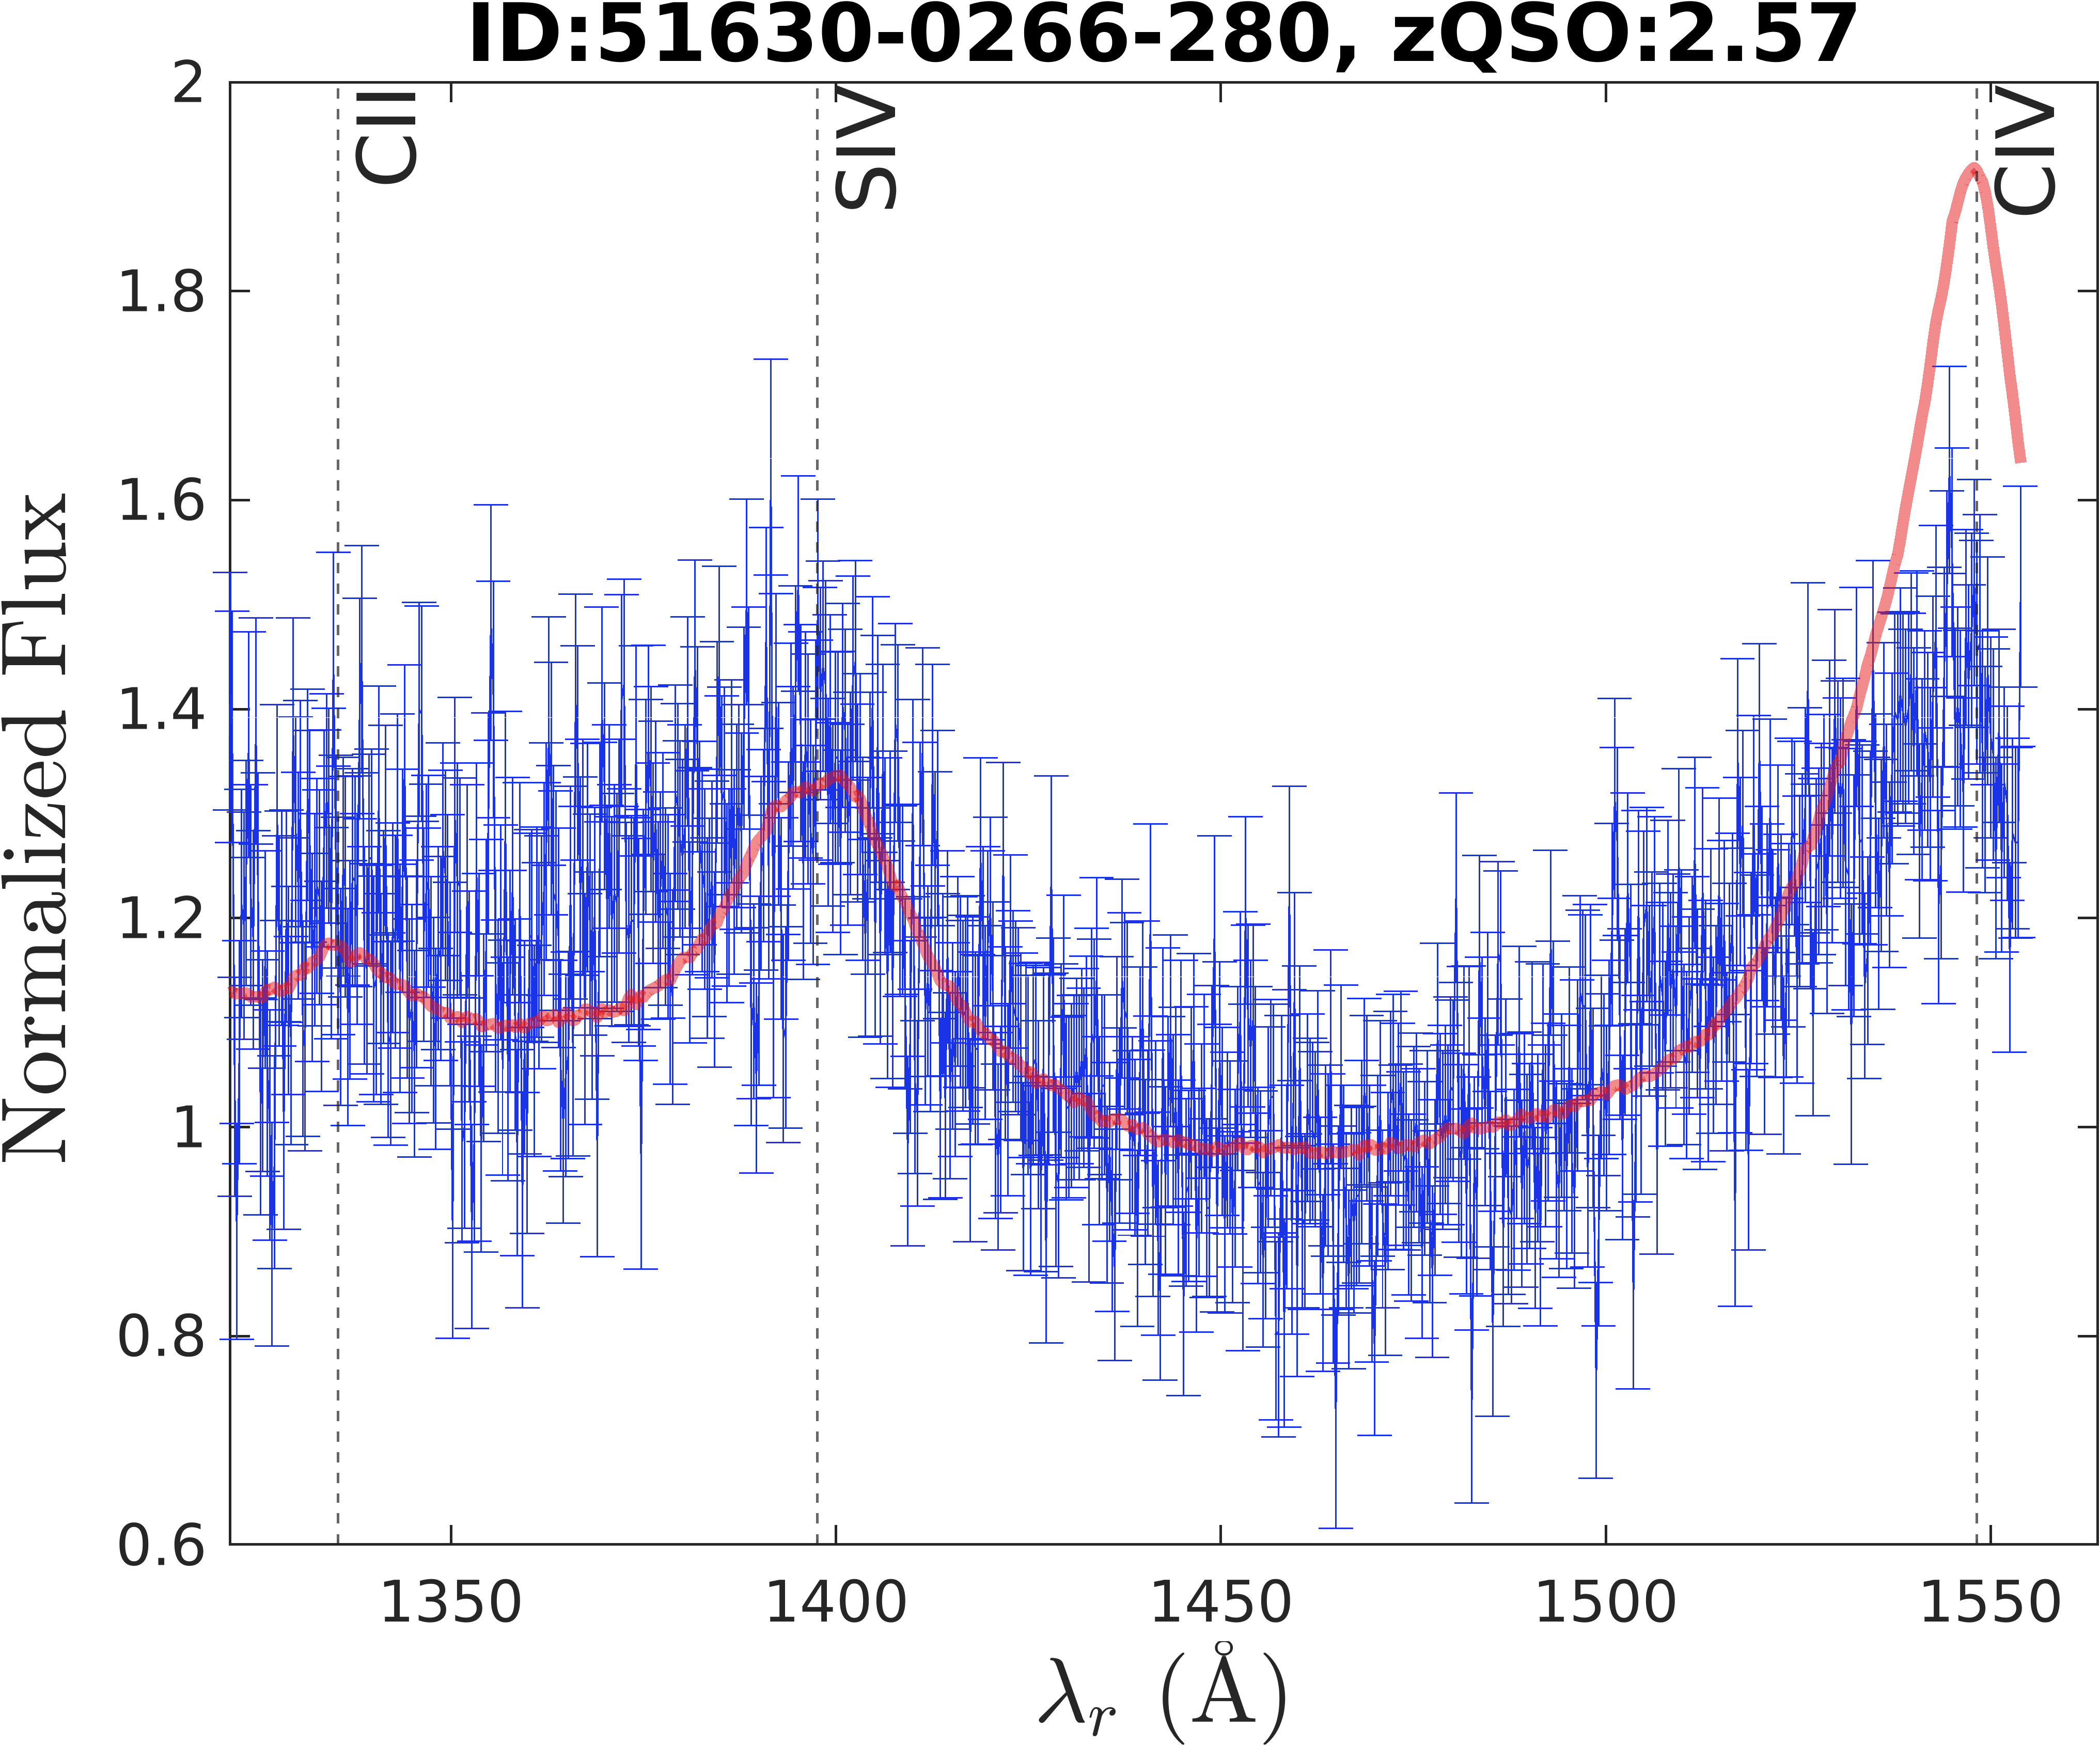
\includegraphics[width=\linewidth]{figs/QSO-1.png}
  \caption{An example learned quasar emission function (thick red curve) with the normalised observed flux (blue curve). The SDSS DR7 quasar has QSO-ID 51630-0266-280 and redshift $2.57$.  The thick red curve is our learned quasar continuum. The thick blue
   curve is the smoothed observed flux. The two thin blue curves show the boundaries on the $1-\sigma$ observed flux from the noise. Note that we search for absorbers starting 3000\kms\ red-ward of the quasar's redshift, so the moderate failure to match the quasar emission line in this case does not lead to an artificial preference for \civ\ absorption.
  }
  \label{fig:mu}
\end{figure}


% Gaussian Processes give us a probability distribution over functions
% compared to a multivariate Gaussian distribution which provides a
% distribution over vectors.
Our method extracts some information, even from
noisy data, so we do not enforce a minimum signal to noise in our search.
Our pipeline naturally gives low likelihoods to low SNR spectra  during the training.
We can completely specify a GP by its mean and correlation functions (analogous to the first two moments of a Gaussian distribution).
% GP
We define the mean function $\mu$ by:
\begin{equation}
  \mu(\lambda) = \langle y(\lambda)  \rangle.
\end{equation}
$\lambda$ is the rest-frame wavelength and $y(\lambda)$ is
the observed rest-frame flux for the training set spectra, after
applying a mask for missing pixels. Angle brackets $\langle \rangle$
denote an average.
Before computing this average over the training set, we normalise the quasar flux
and the flux variance  so that they
have a median value of unity in the normalization range.
This normalization is needed
so that the GP model needs not be concerned with variations in quasar brightness.
We choose the range from 1420\AA \ to 1475\AA \ as it contains no prominent emission lines \citep{Zhu13, hamann17, Monadi21}.
We have also confirmed empirically that normalization range produces the best score when applied to our validation set.
%never saw a better ROC curve, purity, or completeness.

%Finally, by considering non-NaN values in the rest frame interpolated fluxes, for each pixel in our wavelength grid
%we take the average over all of the training set quasar fluxes.
% \begin{equation}
%   \mu(\lambda_i) = \mathtt{nanmean}(\vec{y})
% \end{equation}

The GP covariance function, which describes the correlation between flux values at two separate wavelengths, $\lambda$ and $\lambda^{\prime}$, is given by:
\begin{equation}
     K(\lambda, \lambda') = \langle (y(\lambda) - \mu(\lambda)) (y(\lambda') - \mu(\lambda'))  \rangle,
    \label{eq:gp_mean_cov}
\end{equation}
Most applications of Gaussian processes assume a simple template for the covariance, such as the exponential squared kernel \citep{GPbook}.
However, the complex shape of quasar continua means they are not
well described by these simple covariance functions.
Instead we dynamically learn a matrix form of the covariance function.

We bin quasar spectra linearly in wavelength, from $1310 - 1555$ \AA,
with $\Delta \lambda = 0.5$. $N_{pixel}$ is given by:
\begin{equation}
  N_{pixel} = \frac{Max(\lambda_{learn}) - Min(\lambda_{learn})}{\Delta\lambda},
\end{equation}
and so we have a maximum of $N_{pixel} = 490$ bins per spectrum.
%The covariance matrix, $\mathbf{K}$, has size $N_{pixel}\times N_{pixel}$.
A very fine $\Delta \lambda$ is not desirable because it increases the size of
 $\vec\mu$ and $\mathbf{K}$ and thus is more computationally expensive. On the other hand a very coarse $\Delta\lambda$ cannot capture enough information from the quasar
 spectra. The optimum $\Delta\lambda$ in \cite{romanDLA} and \citep{mfDLA}
was 0.25\AA. After some iterations, we found that $\Delta\lambda=0.5$\AA\ is the optimum value for the redder spectral region we examine here.

Without further structural assumptions on $\mathbf{K}$ we would
learn a matrix of $N_{pixel}^2 \sim 2.4 \times 10^5$ elements.
To circumvent this, we use a low rank decomposition:
\begin{equation}
  \mathbf{K} = \mathbf{M}\mathbf{M}^{\top},
  \label{eq:K}
\end{equation}
where $\textbf{M}$ is a $N_{pixel} \times k$ matrix.
$k$ is a positive integer.
Larger $k$ models allow for higher fidelity modelling of $\mathbf{K}$.
%More than 99\% of the variance of $\mathbf{K}$ after decomposing it
%with $k=10$ will be captured.
Following \cite{romanDLA}, we set $k=20$. We also checked
$k=19$, $21$, and $22$, finding that our results were insensitive to this choice. %However, increasing/decreasing $k$ did not give
%us a better performance and we kept the size of covariance matrix decomposition
% at 20.
%Therefore, here we use $k=20$ similar to \cite{romanDLA}.}

We learn $\mathbf{K}$ by maximising the likelihood of observing the (\civ-free) training data given the null (or absorption free) model.
Optimisation of $\mathbf{K}$ was done using \texttt{minFunc}, a Matlab function for unconstrained optimization of differentiable real-valued multivariate functions using line-search methods\footnote{\href{https://www.cs.ubc.ca/~schmidtm/Software/minFunc.html}{https://www.cs.ubc.ca/~schmidtm/Software/minFunc.htm}}.
Fig. \ref{fig:K} shows the learned covariance matrix.
\begin{figure}
  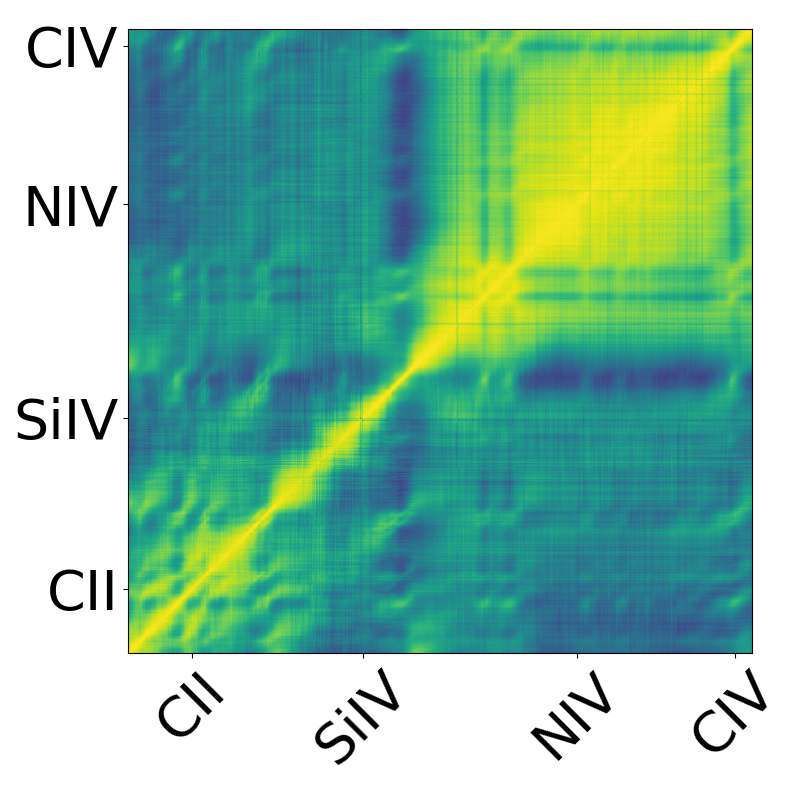
\includegraphics[width=\linewidth]{figs/covariance_matrix-M2.png}
  \caption{Learned covariance matrix for our null model. Brighter pixels show stronger correlations and darker regions weaker ones. The wavelengths of prominent emission lines are labelled. The bright diagonal implies stronger correlations between pixels at smaller wavelength separation.}
  \label{fig:K}
\end{figure}

% examle and ref to RomanDLA
Having learned the mean quasar function, $\mu$, and
the covariance matrix, $\mathbf{K}$, we can write
the GP model for the quasar
emission function, trained on the observed data, as a multivariate Gaussian distribution:
\begin{equation}
\begin{split}
  p(f(\lambda)) & = & \mathcal{GP}(\mu(\lambda), K(\lambda, \lambda'))  \\
  & = & \mathcal{N}(f; \mu(\lambda), K(\lambda, \lambda')),
  \label{eq:conti}
\end{split}
\end{equation}
The mean vector $\mu(\lambda)$ and covariance matrix $K(\lambda, \lambda')$ are evaluated at each wavelength, $\lambda$. $\mathcal{N}$ denotes the Gaussian distribution:
\begin{equation}
\mathcal{N}(f; \mu, K) = \frac{1}{\sqrt{(2\pi)^d det(K)}}exp\Bigl( -\frac{1}{2} (f-\mu)^{\top} K^{-1} (f-\mu)\Bigr),
\end{equation}
where $d$ is the dimension of $f$. Therefore,
given a desired grid $\lambda$, the prior distribution for our noisy observations, $y(\lambda)$, will be:
\begin{equation}
  p(y| \mu, K, v ) = \mathcal{N}(y; \mu, K + V),
  \label{eq:GPprior}
\end{equation}
where we used the property of Gaussian processes that the
sum of two Gaussian functions (here observational noise and $f$ which is a GP)
is a Gaussian. $V$ is the diagonal matrix of the observed photon noise for all $\lambda$.\footnote{The 3rd column of the SDSS fits tables
for observed spectra contains inverse noise variance $1/\sigma^2(\lambda)$.}
Assuming our observations, $y(\lambda)$,  are independent  and
drawn from the noisy observation prior of Eq. \ref{eq:GPprior}, we can write the combined likelihood of the training set as:
 \begin{equation}
  p(y | \lambda, \mu, V, M) = \prod_{i=1}^{N_{spec}}\mathcal{N}(y_i; \mu, K+V_i).
 \end{equation}
Now we can maximise the likelihood (see  section 5.3 of \cite{romanDLA} for
 details) and learn $\mu$ and $M$ in Eq. \ref{eq:K} based on the combined
 information within the observed fluxes and noise in our training set.

  %% multi absorber

  % To build the absorption function of multiple absorbers, we use element-wise product
  % of 5 absorbers:
  % \begin{equation}
  %   \vec{a}_{(k)} = \prod_{i=1}^{4}\vec{a}(\vec{\lambda}; \zciv, \nciv, \sciv).
  %   \label{eq:a_k}
  % \end{equation}
  % We did not go beyond 4 absorbers because of the distribution of the number of
  % absorbers in C13 catalogue. 42\% of spectra in C13 have at least 1 absorbers,
  % 14.8\% of them have at least 2 absorbers, 4.6\% of them have at least 3 absorbers,
  % and finally 0.4\% of them have more than 4 absorbers.
    % \begin{figure}
  %   \includegraphics[width=\linewidth]{figs/Dist_Num_absorbers.png}
  %   \caption{The distribusion of number of absorbers.}
  %   \label{fig:num_absorbers}
  % \end{figure}
  % That is our complete \civ\ model, $\mathscr{M}_{\civ}$, is the union of the models
  % with any arbitrary numbers of absorbers up to 4.

\subsection{Absorption Line Models}
\label{sec:civ-model}

% Bayesian model selection intro + models
We want to decide the probability of
a \civ\ doublet in the observed spectrum of a quasar given $y(\lambda)$ under our null GP model $\model_N$.

% \subsection{Model Posterior}
Our data  is composed of the observed wavelengths $\lambda$,
their corresponding
observed quasar flux $y( \lambda)$, and their corresponding
 observed noise $ \sigma(\lambda)$.
We define the data as $\Data = \{\lambda; y( \lambda), \sigma(\lambda)\}$.
Bayes' rule gives the \emph{model posterior}, the probability of each model given the data:
 \begin{equation}
  P_n(\model \mid \Data) =
  \frac{P_n(\Data \mid \model_n)Pr(\model_n)}{
     \sum_n P_n(\Data \mid \model_n)Pr(\model_n),
  }.
  \label{eq:model_selection}
\end{equation}
$P_n$, the normalised posterior probability of models, is the ultimate product of our catalogue.

We define three models:
\begin{itemize}
  \item $\model_{N}$ models the quasar continuum without absorption (Eq. \ref{eq:conti}).

\item $\model_{D}$ is a model containing
exactly one \civ\ doublet. $\model_D$ is built by convolving $\model_N$ with the absorption function (Eq. \ref{eq:a}) for all observed wavelengths:
\begin{equation}
  \model_{D} = a(\lambda) f(\lambda)\,.
  \label{eq:model_D}
\end{equation}

\item $\model_{S}$ is a singlet model containing exactly one generic singlet absorption line. For simplicity, we implement $\model_S$  using the same Voigt profile as $\model_D$, but including only the 1548\AA\ absorption line
\begin{equation}
  \model_{S} = a_{1548}(\lambda)  f(\lambda)\,.
  \label{eq:model_s}
\end{equation}
\end{itemize}

We add this singlet model, in addition to the \civ-free and \civ\ doublet models, as the relative rarity of singlet absorbers means that our Bayesian framework often prefers a high probability of a \civ\ doublet to the null model. Thus a very strong singlet line like
\ion{Fe}{II}, \ion{Al}{II}, \ion{Al}{II}, \ion{Si}{II} can be mis-identified as a \civ\ doublet.
The singlet model, $\model_S$, provides an alternative to both $\model_N$ and $\model_D$ for these lines.
%There are cases that a fit with
%one component better describes the spectrum (data) than a fit  with doublet \civ.
Fig. \ref{fig:sngl} shows an example, where a
a noise fluctuation and a strong line happen to have a velocity separation similar to a \civ\ doublet.
For this spectrum we have:
\begin{itemize}
\item $\log(P(\model_{N} \mid \Data))= -297.8216$,
 \item $\log(P(\model_S \mid \Data))= -250.1609$.
\item $\log(P(\model_D \mid \Data))= -257.1906$,
\end{itemize}
Although the doublet model is not a very good fit, the null model is even worse. Thus without the singlet model, $\model_S$, our pipeline would incorrectly prefer the doublet model and detect a \civ\ absorber.
% posterior probability (Eq. \ref{eq:model_posterior}) for \civ\ doublet model, $\model_D$, would be
%   $P(\model_D)\sim 1$.

\begin{figure}
  \centering
  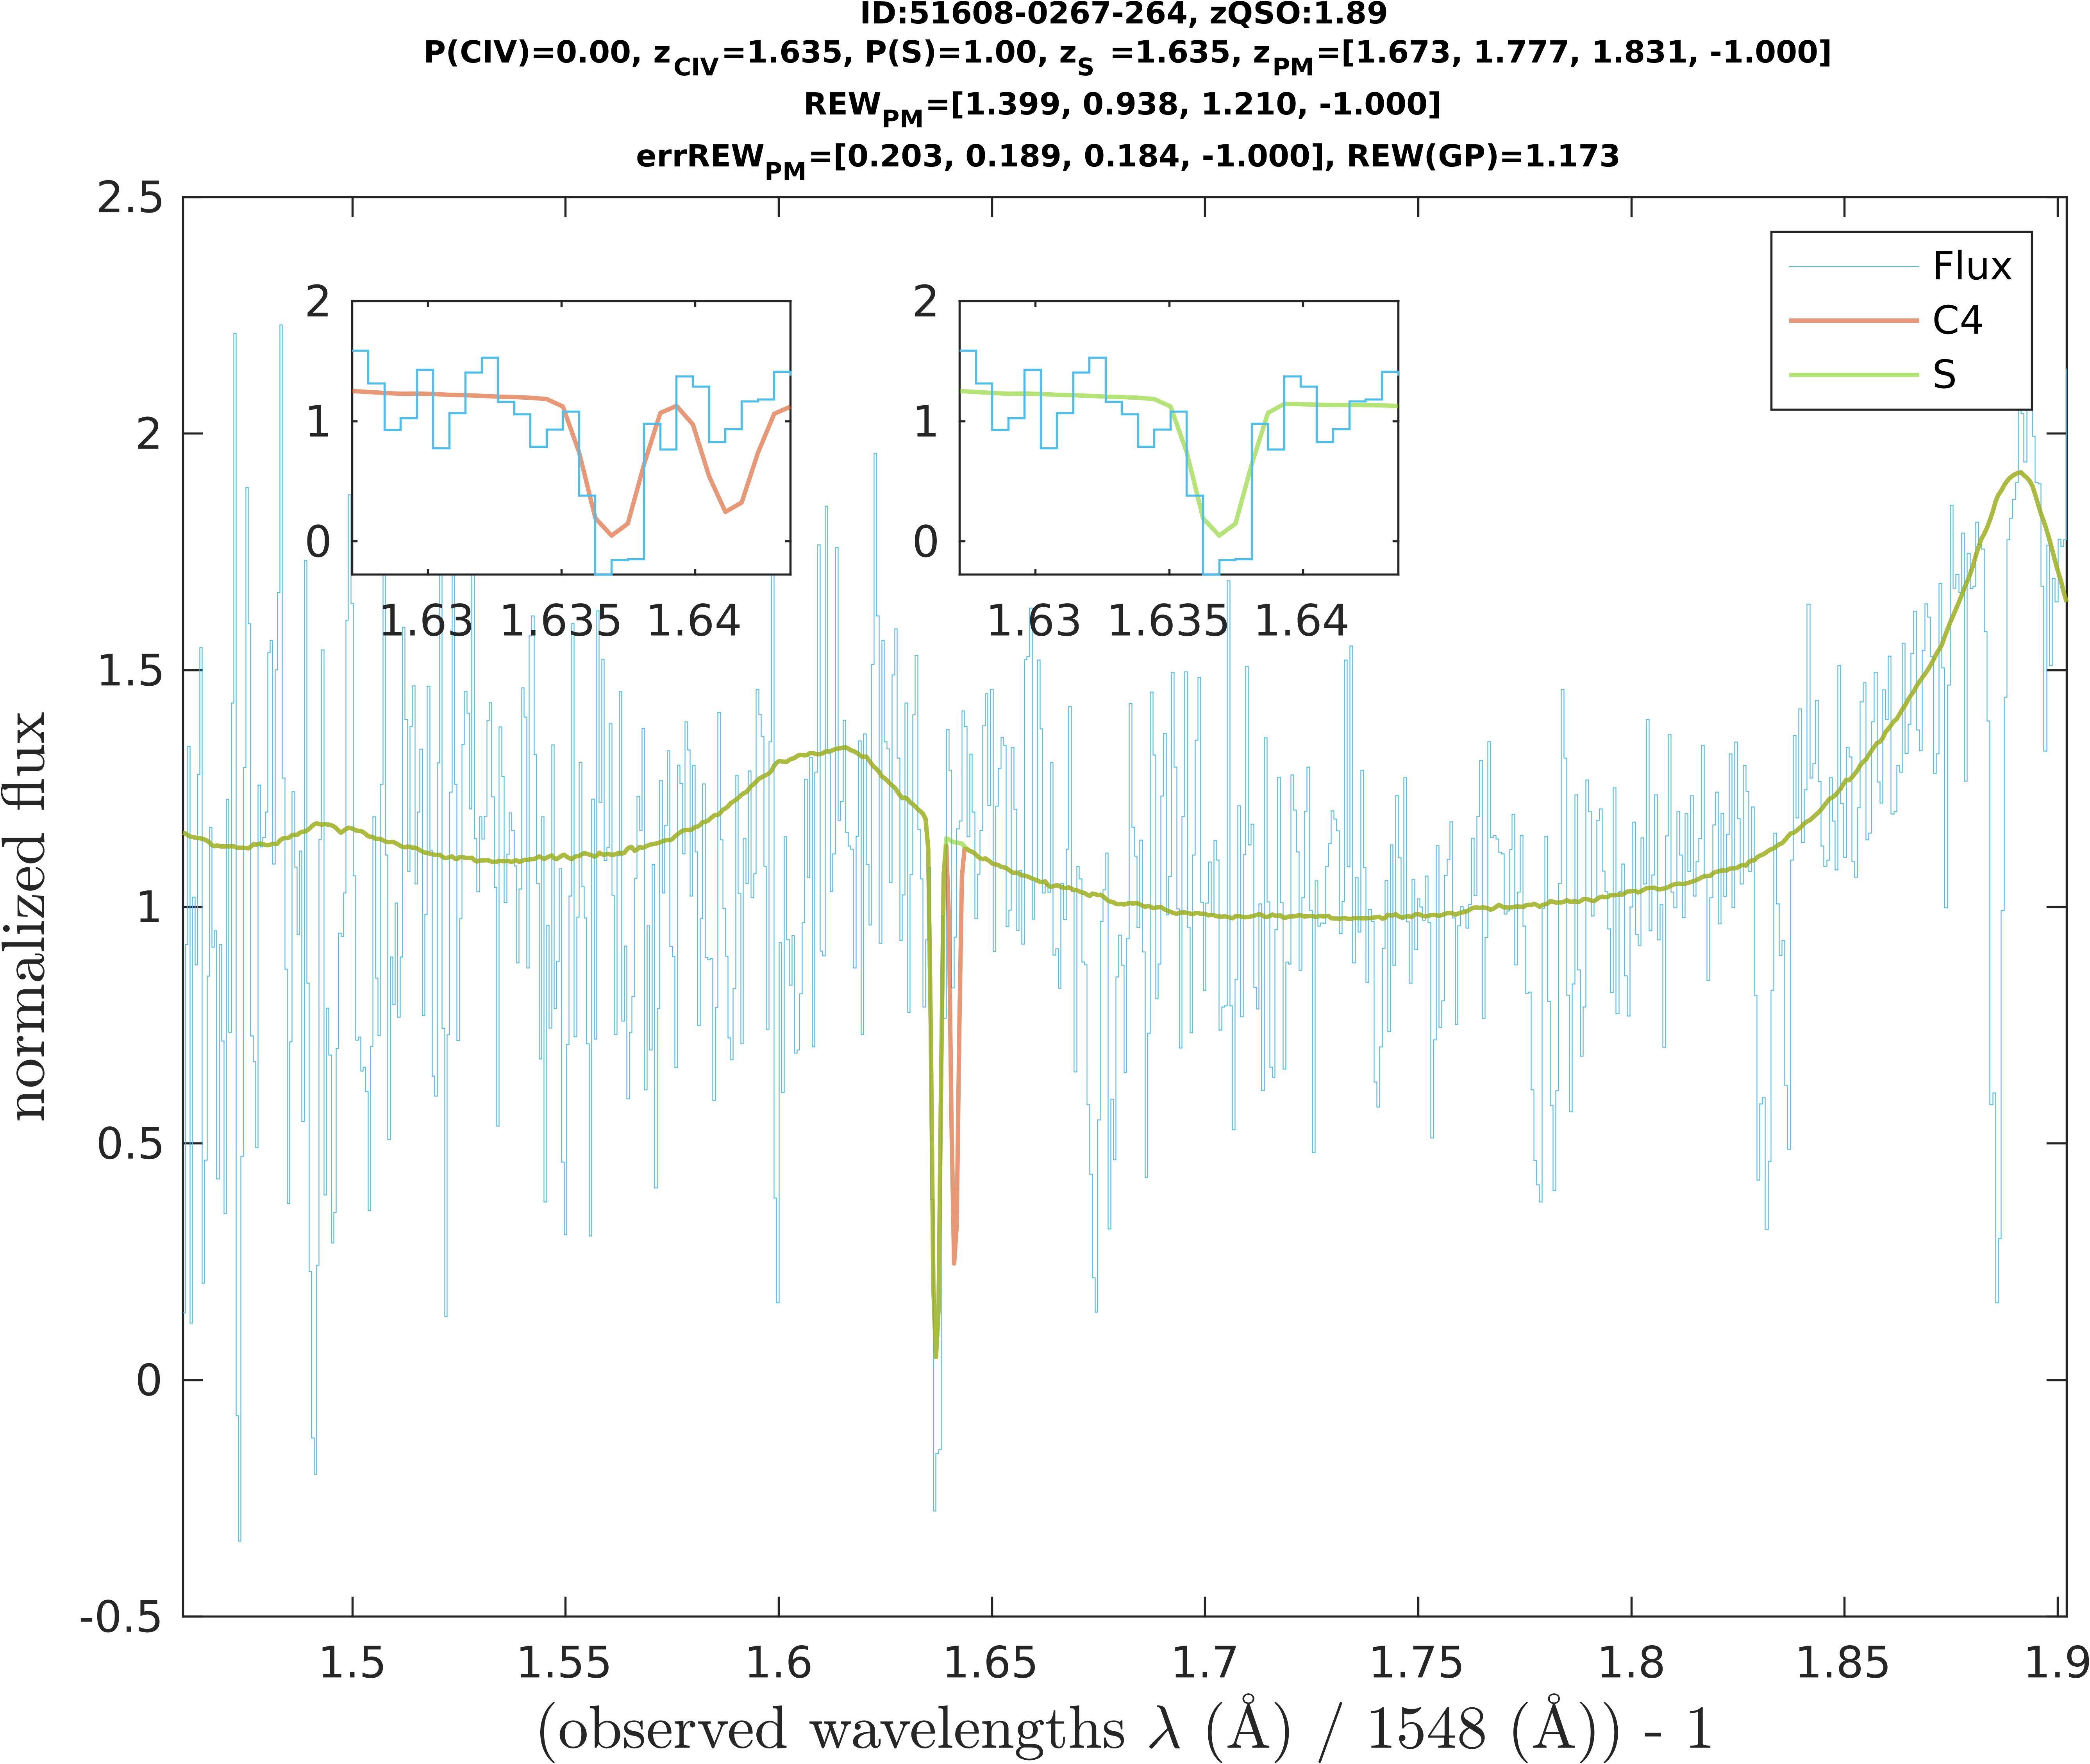
\includegraphics[width=\linewidth]{figs/ind-4-c4-1.png}
  \caption{An example of a spectrum where the singlet model, $\model_S$, is preferred over the \civ\ doublet model $\model_D$, which is in turn preferred over the null model $\model_N$. Zoom-in
   panels show the best fit doublet model ($\model_D$) and best fit singlet models ($\model_S$) in a smaller redshift range around the candidate detection.
   %This demonstrates why we need this alternative model to lower our false positive detection rate and obtain a pure catalogue.
   If we did not have $\model_S$, our pipeline
   would have incorrectly detected a \civ\ absorber at $\zciv = 1.635$. }
     \label{fig:sngl}
\end{figure}

% We normalise the model posteriors (Eq. \ref{eq:model_selection}), we can normalise them to select the best model describing our data:
% \begin{equation}
%   P_{n}(\model | \Data) =  \frac{P(\model|\Data)}{\sum P(\model|\Data)}.
%   \label{eq:model_posterior}
% \end{equation}
% Eq. \ref{eq:model_posterior} ensures that the detection of a \civ\ absorption is complement to non-detection and
% detecting something similar to a \civ\ but with a single line absorption profile:
% \begin{equation}
%       P_n(\model_D | \Data) = 1 - P_n(\model_{N}|\Data) - P_n(\model_S|\Data).
%       \label{eq:PnD}
% \end{equation}
%\spb{I don't think we need this: it follows trivially from Bayes rule above.}

\subsection{Model priors}
\label{sec:modelpriors}

 To calculate the model posterior (Eq. \ref{eq:model_selection}),
  we need model priors, $Pr(\model)$, for each of the three models.
%  A model prior is our level of faith on that model
%   prior to do the model selection.
% We calculate the prior for \civ\ doublet model required
% in multiple searches discussed in section
% \ref{sec:modelpriors}.
 We set priors for the \civ\ doublet, $\model_D$, using population statistics from our training set, the PM catalogue of C13.
 We count the fraction of spectra with absorbers at $z<\zqso + 30000 /c $,
 where $c$ is the speed of light in \kms.
 This small increase in our lower limit for the
 absorption redshift accounts for any possible error in estimating
 of redshift that is obtained from SDSS pipeline.
For simplicity, we used the same prior for the singlet and doublet line models, that
is we set $Pr(\model_S)=Pr(\model_D)$.
There are no single line catalogues for this data and using equal
priors ensures that whichever model is the best fit will be used.
Following the same logic, we use the  parameter priors in
section \ref{sec:model_likelihood} when we calculate model likelihoods.
That is $P(\theta\mid \model_{S}, \zqso) = P(\theta\mid \model_{D}, \zqso)$,
where $\theta = \{\zciv, \nciv, \sciv\}$.
The prior for the \civ\ free model can be obtained by:
\begin{equation}
  Pr(\model_N(n \civ)) = 1- Pr(\model_D(n~\civ)).
  \label{eq:priorNull}
\end{equation}
We did not include $Pr(\model_S)$ in Eq. \ref{eq:priorNull} to
enable a pointwise model comparison between $\model_D$, $\model_S$
and $\model_N$. Especially when searching for multiple absorbers, our
main purpose is deciding the probability of detection or non-detection
of \civ\ absorbers in a spectrum.
Furthermore, the small shift in the normalization of model
priors is several orders of magnitude smaller than the effect
of normalising the model posteriors in Eq. \ref{eq:model_selection}.

When searching for multiple absorbers, in spectra where there is already a detection, we use the prior probability of spectra with $n-1$ \civ\
 absorbers having $n$ absorbers:
\begin{align}
    Pr(n~ \civ) &=P(n~\civ|n-1~\civ)\\
    &= \frac{P(n-1 ~\civ \cap  n ~\civ)}{P(n-1 ~\civ)} \\
    &= \frac{P(n~\civ)}{P(n-1~\civ)}\,.
\end{align}
The equality follows as the intersection between the set with
 n \civ\ and the set with  n-1 \civ\ will be the set of quasars with   n \civ\ absorbers. Fig. \ref{fig:prior} shows the $\model_D$
priors we used for different searches as a function of $\zqso$.
When the redshift increases all of the priors reach a plateau  after $\zqso \sim 3$.
There is a  decrease from Pr(1 CIV) to the
subsequent priors so that $Pr(7 ~\civ) <15\%$.
Absorbers are correlated, so the prior for detecting $k$ absorbers in a spectrum given a redshift is larger than $Pr(1 \civ)^k$.

% \rmon{Need to explain priors for column density, redshift and sigma here. OPtimization text}

\begin{figure}
  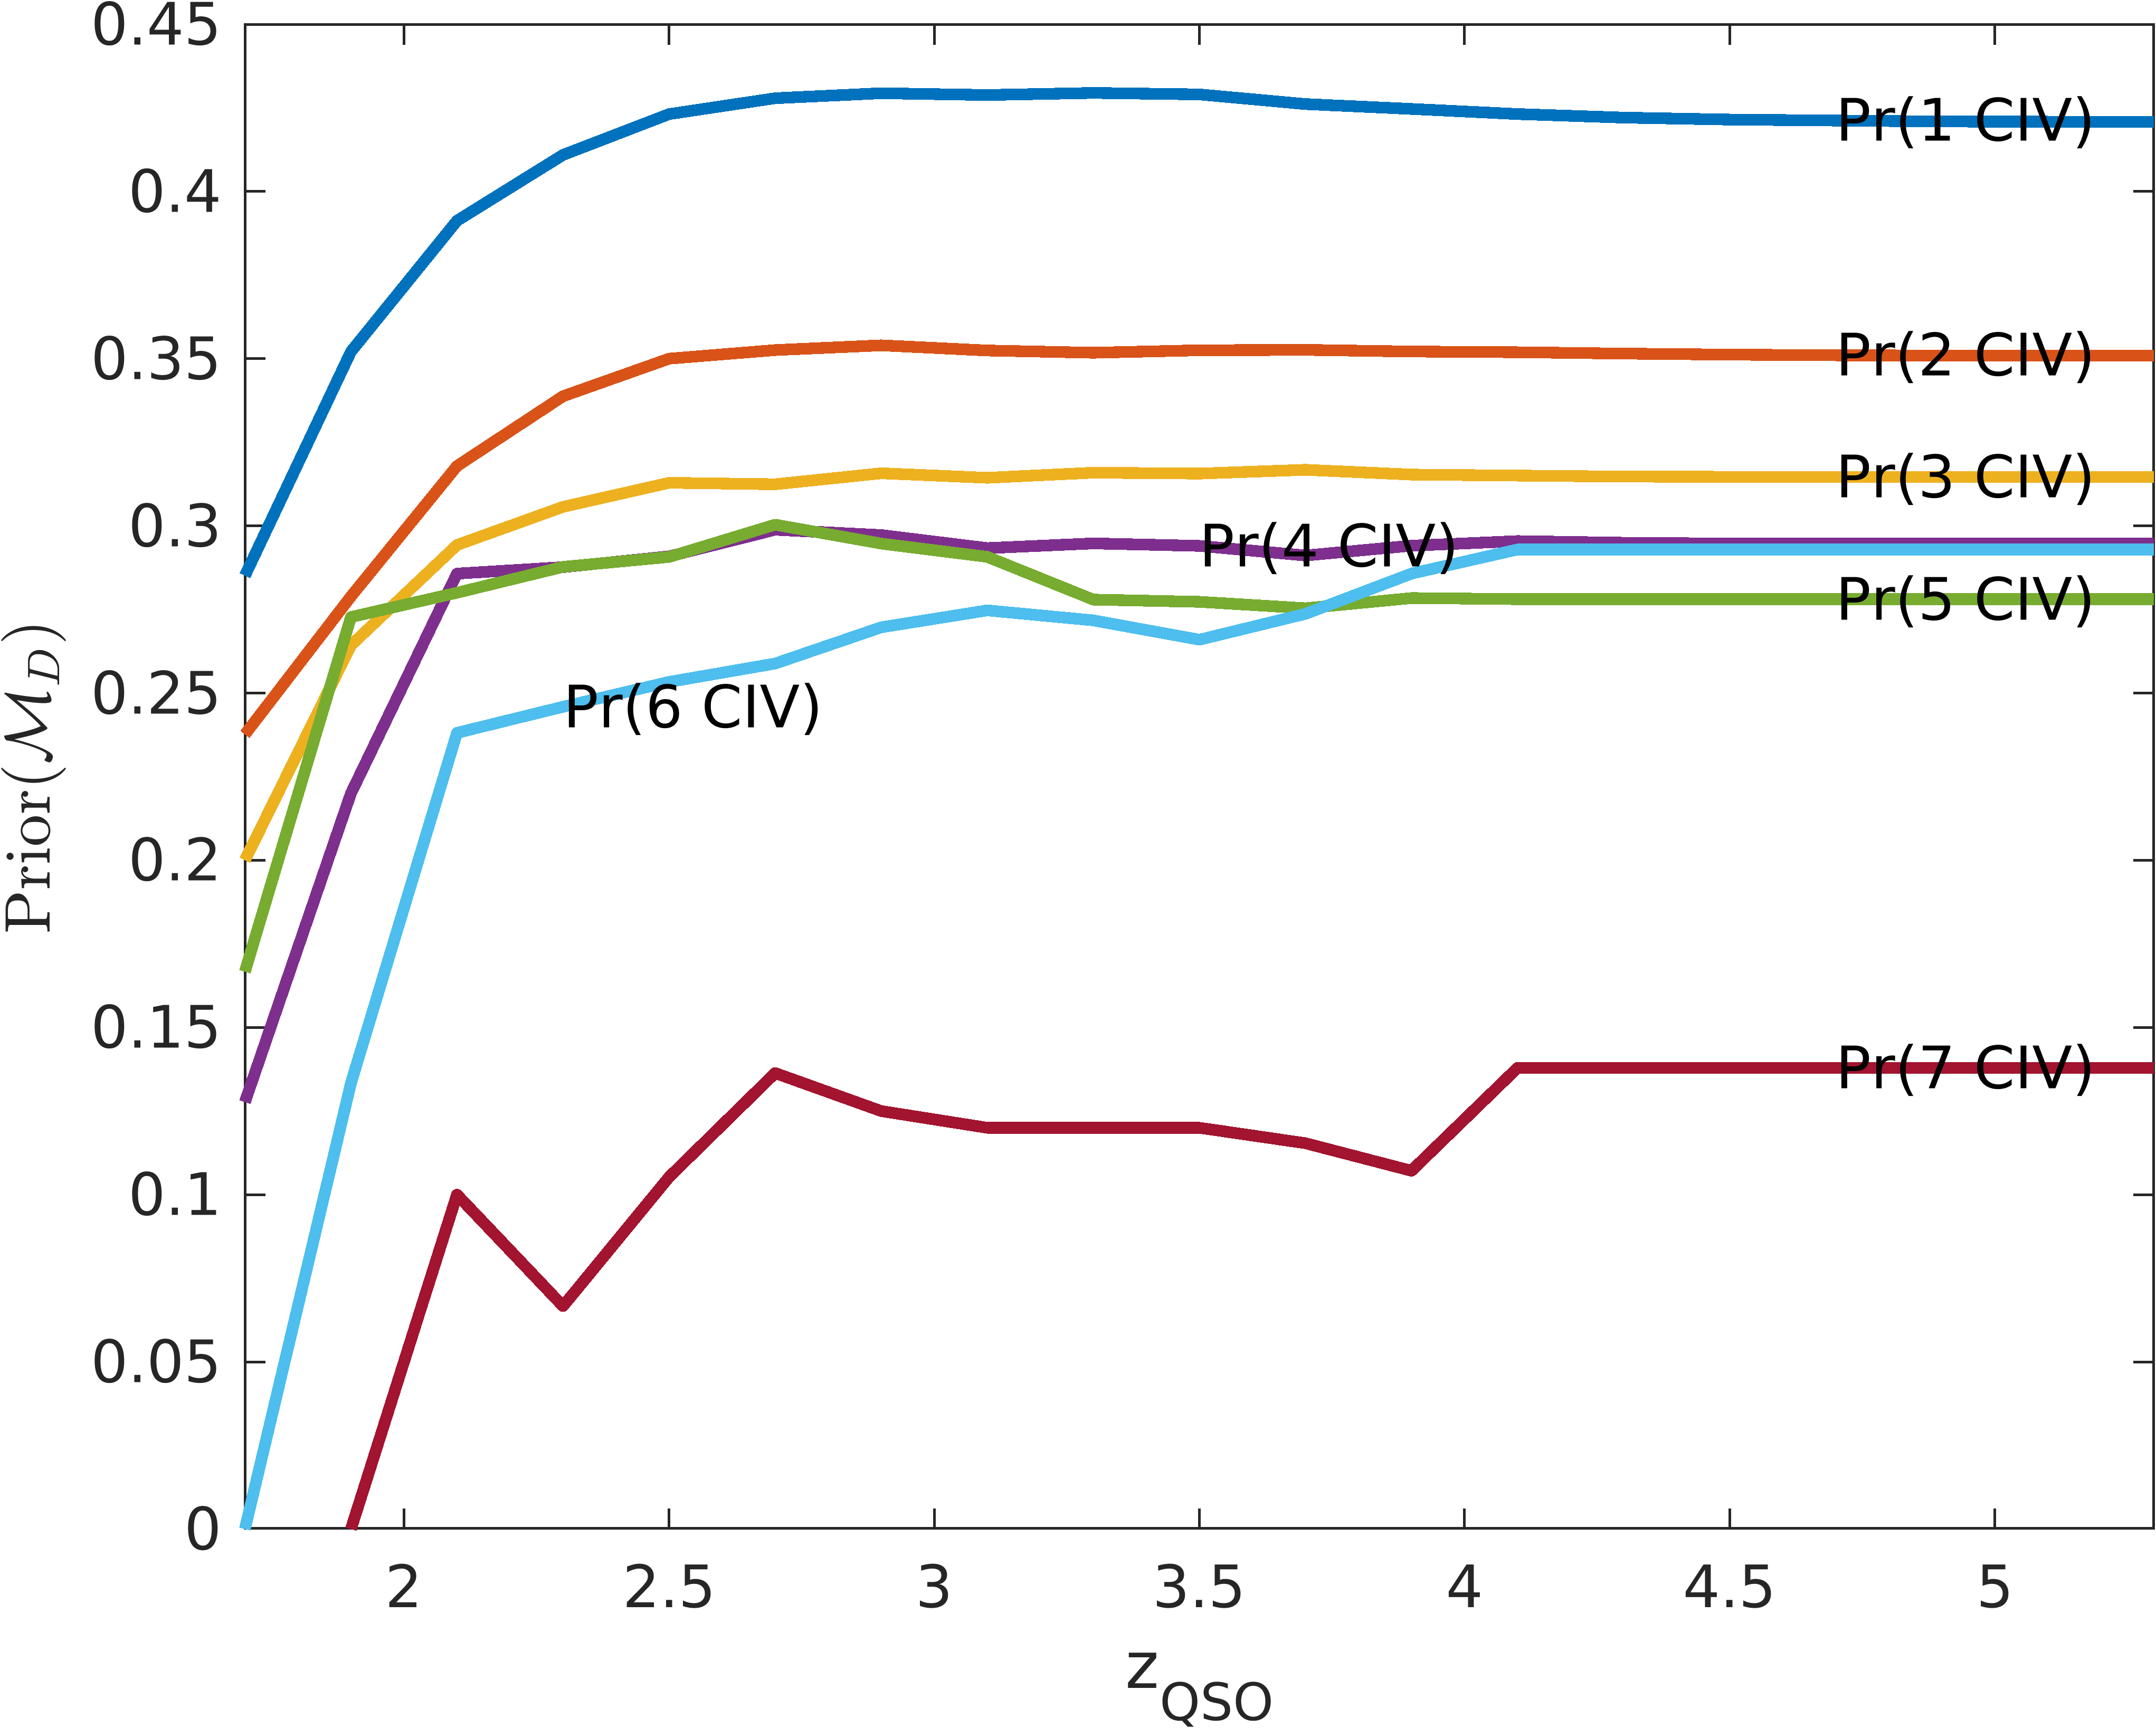
\includegraphics[width = \linewidth]{figs/Priors.png}
\caption{Prior probability %for $\model_D$ %It is for M_S as well!
for a spectrum containing $n$ \civ\ absorbers as a function of redshift, for $n = 1 - 7$. We use the average number of absorbers in the PM spectrum in our wavelength search range.
% having a redshift smaller than  $\zqso + 30,000/c$.
\civ~is a priori more likely as $\zqso$
increases, but reaches a plateau at $\zqso \sim 2.5-3$.
This is because the possible wavelength range
is shorter for low $\zqso$ as the 1548\AA emission
line is outside the SDSS wavelength coverage.}
\label{fig:prior}
\end{figure}

\subsection{Model Likelihood}
\label{sec:model_likelihood}

The model likelihood, $P(\Data \mid \model)$, in Eq.~\ref{eq:model_selection} is
the probability that the observed data, $\Data$, have
been generated by a considered model, $\model$, after marginalising
the model parameters.
%which means we have accounted for any possible configuration for our considered model.
We do the marginalisation over a prior distribution for each parameter in the model:
\begin{equation}
   P(\Data \mid \model) =
   \int P(\Data \mid \model, \theta) P(\theta \mid \model) d\theta.
   \label{eq:marginal_params}
\end{equation}
Here $P(\Data \mid \model, \theta)$ is the likelihood of the data being generated
by model $\model$, if the model has a certain set of parameters $\theta$. We
use the prior probability distribution of $P(\theta \mid \model)$ from Eq. \ref{eq:marginal_params}
to integrate out all of the possible $\theta$ and obtain a
parameter-independent model likelihood. $\model_{N}$ has no
free parameters, but $\model_D$ and $\model_S$ have three free parameters:
1) absorption redshift ($\zciv$), 2) column density of \civ ($\nciv$), and 3) Doppler sigma parameter ($\sciv$).

We need to have priors for each of these
parameters to
perform the integral in Eq. \ref{eq:marginal_params}.
A parameter prior is the probability with which may have a parameter value
given that a model is true.
In the
implementations of this Bayesian approach for detecting DLAs in quasar spectra \citep{mfDLA, mfDLA16},
the prior distribution of the required parameters (i.e. column density and absorber red-shift)
  were learned from the previous catalogues.

  %  N
  One of the input parameters in the Voigt profile\footnote{
  See \texttt{voigt\_IP.c} in our github repository for further details.}
  is the absorber column
  density, $N_{\civ}$.
  Following \cite{romanDLA} and \cite{mfDLA}, we need to sample a column density distribution and integrate model priors to obtain model likelihoods (see Eq. \ref{eq:model_evidence}).
%   We started by the a column density lower limit ($N_{\civ}=14$)
%   larger than the minimum one reported
The column density range detected by C13 was $12.88< \log_{10} \nciv <15.8$. After some experimentation, we chose a slightly larger range: $12.5 < \log_{10} \nciv < 16.1$, which maximised the performance on our validation set. This slightly wider range of column densities, compared to the PM catalogue, has a two-fold benefit. First, the column densities in the PM catalogue are often lower limits. Second, our SDSS DR12 catalogue has a larger dataset and thus may contain weaker or stronger absorbers, outside of the detected range in the PM catalogue. We thus used a composite probability density function consisting of:
    (1) the $\nciv$ probability density function from the reported values in the PM catalogue  and
    (2) a uniform probability density function in the same range.
  We have also confirmed that our column density prior sample reproduces a rest equivalent width distribution that is not very off the rest equivalent width distribution reported in the PM catalogue for the 1548\AA\ line.

  % sigma
We also need a prior for the Doppler broadening parameter $\sigma_v$.
The typical temperature for the intergalactic medium is $\sim 10^4-10^5$
K, which gives a $\sigma_v \sim 2.6 - 8.3$ \kms.
However, at the low resolution of the SDSS spectra ($\sim 150$ \kms), it is difficult to detect single absorbers with this velocity dispersion. Instead, absorbers are frequently clustered or blended into a system with a larger effective
$\sciv$. By experimenting with different ranges for $\sciv$
we chose upper and lower bounds for $\sciv$ as $35$ and $115$ \kms. This range was chosen so that we are sensitive to a similar rest equivalent width as the PM catalogue. Rest equivalent widths (REW) are computed using:
\begin{equation}
  REW(GP) =  \int (1 - a_{1548})d\lambda.
  \label{eq:rewgp} %\int \frac{C- C a_{1548}}{C} d\lambda =
\end{equation}
Here $a_{1548}$ is the absorption function for our 1548\AA\ line from the doublet model, $\model_D$, and we compute the REW from our sampled $\nciv$ and $\sciv$.
%In Eq. \ref{eq:rewgp}
%$C$ is the continuum obtained from the null model,
%$\model_N$ and


% redshift
We imposed a uniform prior distribution on the absorber redshift, $\zciv$. The lower limit is the redshift at which the 1548\AA\ line is at the minimum observed wavelength
or $1310(1+\zqso)$,\footnote{To avoid possible confusion with any OI, SiII absorption pairs, see C13.} whichever is longer. Therefore:
\begin{equation}
  1+ z_{min} = \max\left[\frac{\min(\lambda_{obs})}{1+\zqso}, \frac{1310(1+\zqso)}{1548}\right].
  \label{eq:zmin}
\end{equation}
We also require a small velocity separation between the absorber and the quasar, to ensure that we are not finding intrinsic \civ\ absorbers around the host galaxy of the quasar:
\begin{equation}
  z_{max} = \zqso - \frac{\delta v}{c}(1+\zqso).
  \label{eq:zmax}
\end{equation}
We considered $\delta v$ $1000$ to $5000$ \kms, and achieved the best validation performance when $\delta v =3000$ \kms.

We assume that $\nciv$ and $\sciv$ are independent from $\zqso$, although
$\zciv$ depends on $\zqso$ as described in Eq.~\ref{eq:zmin} and Eq.~\ref{eq:zmax}.
We calculate the marginalised model likelihood by integrating the model priors for $\model_{D,S}$ as:
\begin{equation}
  P(\theta \mid \zqso)\dd\theta  \propto P(\zciv \mid \zqso)P(\nciv)P(\sciv).
  \label{eq:pr_model}
\end{equation}
Now we can perform the integral for our absorption models, $\model_D$ and $\model_S$, in Eq. \ref{eq:marginal_params}:
    \begin{equation}
       P(\Data \mid \zqso) \propto
       \int P(\vec{y} \mid \theta, \zqso)
       P(\theta \mid \zqso)\dd\theta.
    \label{eq:model_evidence}
 \end{equation}
However, Eq. \ref{eq:model_evidence} is intractable, so we approximate it
with a quasi-Monte Carlo method. This method selects those $10,000$
samples of $\{\nciv, \sciv, \zciv\}$ with an approximately uniform spatial distribution
from a Halton sequence to calculate the model
likelihood, approximating the model evidence by the sample mean:
 \begin{equation}
     P(\Data \mid \model_{D,S}, \zqso) \simeq
     \frac{1}{N} \sum_{i=1}^{N} P(\Data \mid \theta_i, \zqso, \model_{D,S}).
  \label{eq:model_evidence_qmc}
\end{equation}
We integrated out the parameters, $\theta = \{\zciv,\nciv, \sciv\}$, with
  a given parameter prior $P(\theta \mid \zqso, \model_{D,S})$.
  We use $10,000$ samples: lower sample sizes under-sample the likelihood function, while larger sample sizes cause the code to run slower.
  We considered $10,000 - 50,000$ samples in the validation phase, but found that increasing the number of samples did not significantly improve the validation performance.
  Note that in calculating the model evidence for the singlet model, $\model_S$,
   we use a single component Voigt profile centred in 1548\AA\ (Eq. \ref{eq:model_s}) while for calculating the
  model evidence for the doublet model, $\model_D$, we use a double component Voigt
  profile centred at 1550\AA\ and 1548\AA\ (Eq. \ref{eq:model_D}). We use the same parameter priors for both the singlet and doublet models for simplicity.

\subsection{Multiple Absorber Search}
\label{sec:multiciv}

We use a different approach for detecting multiple absorbers from
\cite{mfDLA}. To obtain the model likelihood of the $k^{th}$ model (ie, the model which includes $k$ absorbers), they calculate:
\begin{equation}
  \begin{split}
  P(\Data\mid \model_{DLA(k)}, \zqso) \propto
    \int P(D \mid \model_{DLA(k)}, \{\theta_i\}_{i=1}^{k})\times \\
    P(\{\theta_i\}^k_{i=1} \mid \model_{DLA(k)}, \Data, \zqso)\dd\{\theta_i\}_{i=1}^{k},
  \end{split}
\end{equation}
where the parameter prior for multiple Damped Lyman-$\alpha$ Absorbers (DLAs) is a multiplication between a non-informative prior
$P(\theta_k\mid \zqso,\model_{DLA(1)})$ and the posterior of the $k-1$ multiple DLA model:
\begin{equation}
  \begin{split}
    P(\{\theta_i\}^k_{i=1} \mid \model_{DLA(k)}, \Data, \zqso) = \\
    P(\{\theta_i\}^{k-1}_{i=1} \mid \model_{DLA(k-1)}, \Data, \zqso)P(\theta_k\mid \zqso,\model_{DLA(1)}),
  \end{split}
\end{equation}
In this paper, instead of reporting probabilities for multiple \civ\ absorbers, we
simplify and report the probability that there is an absorber at a given redshift.
For example, the posterior probability for the $k=3$ model in \cite{mfDLA} does not tell us which of these
$3$ absorbers in $\model_{DLA(3)}$ is most probable, instead reporting the probability that a given spectrum contains some combination of $3$ absorbers.
Fig. \ref{fig:PM1GP1}
shows an example of 3 absorbers found by both our GP catalogue and the PM catalogue.

\begin{figure*}
  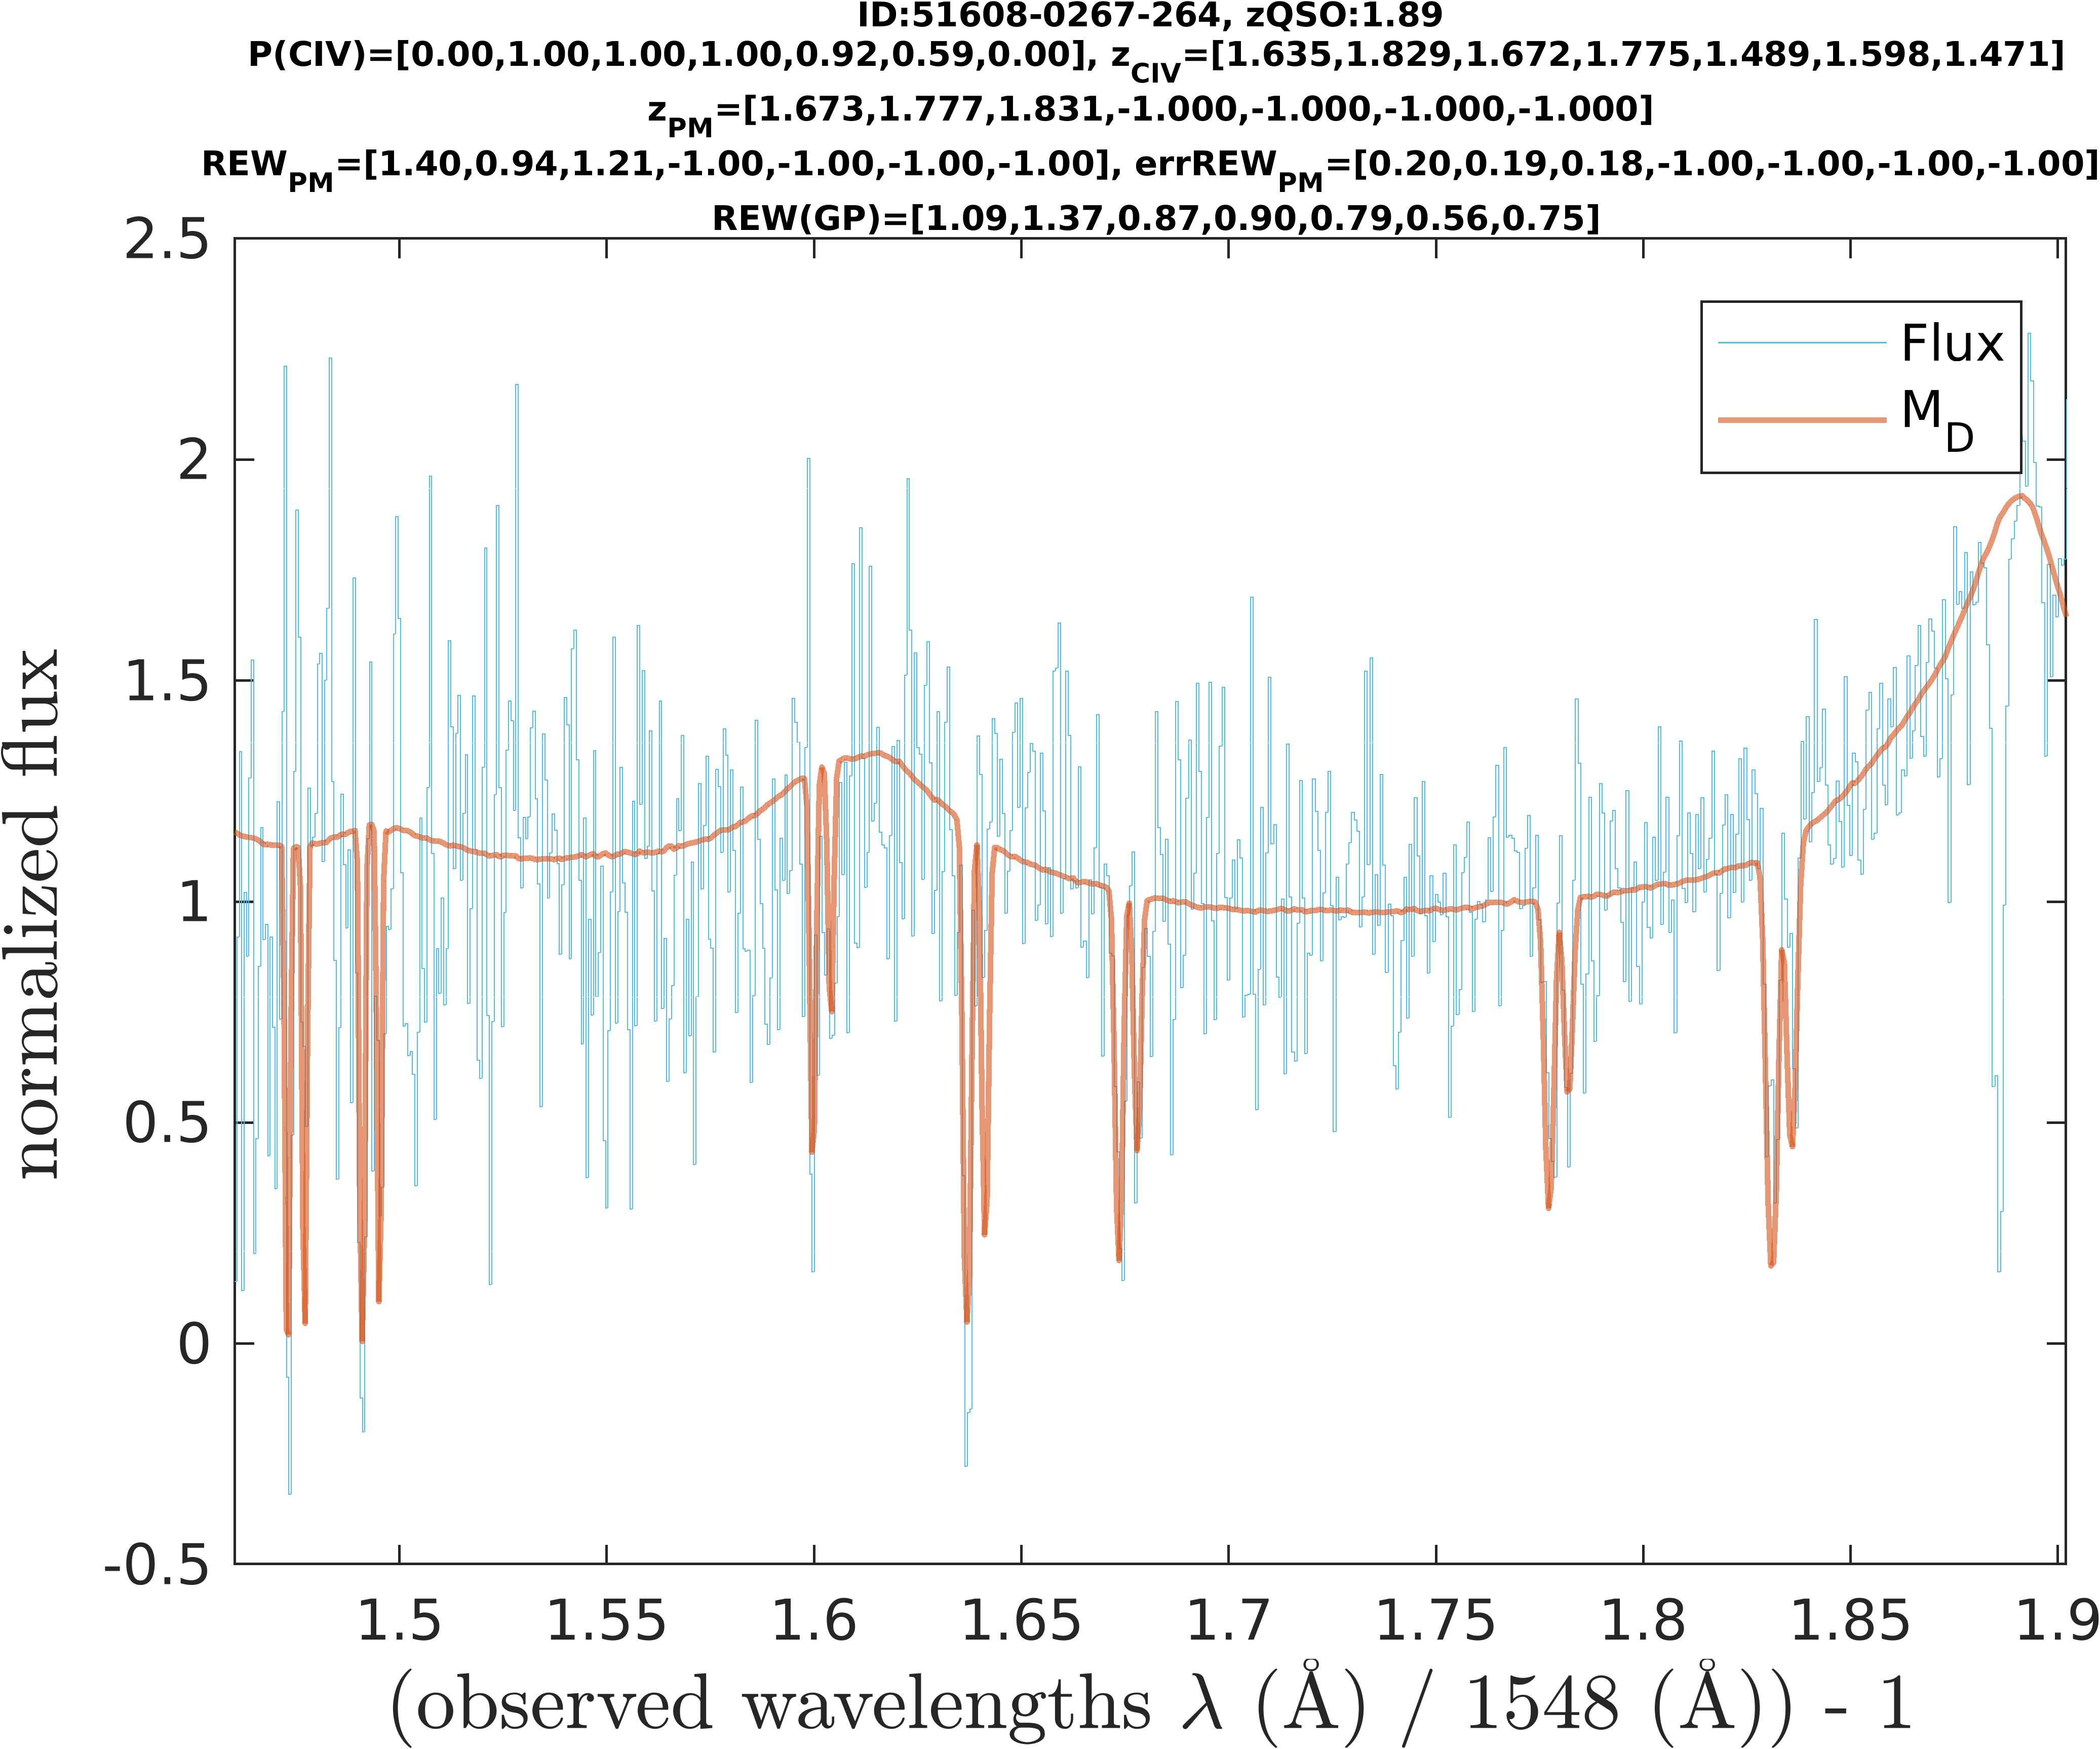
\includegraphics[width=0.75\linewidth]{figs/PM1GP1.png}
  \caption{Example SDSS DR7 spectrum with QSO-ID 51608-0267-264 and $\zqso = 1.89$.
 Both PM and our pipeline find three absorbers. We also find a likely absorber at $\zciv=1.489$ (probability 92\%) that was not detected by PM, likely due to noise in this part of the spectrum.
The probability that our pipeline provides for the existence of \civ absorbers are
 P(CIV)=[1.00, 1.00, 1.00, 0.92], our maximum a posteriori absorber redshift values are
 $z_{CIV}$=[1.829, 1.672,1 .775, 1.489], and our rest equivalent widths from Voigt
 profile integration are REW(GP)=[ 1.37, 0.87, 0.90, 0.79]\AA. In the PM-catalogue the absorber redshifts are
$z_{PM}$=[ 1.831, 1.673, 1.777] and their corresponding rest equivalent widths are
REW(PM)=[1.21$\pm$0.18, 1.40$\pm$0.20, 0.94$\pm$0.19]}

  \label{fig:PM1GP1}
\end{figure*}

Here, we wish to find multiple absorbers in a spectrum. We proceed iteratively, noting that at any point the best fit may be a singlet or a doublet, and mask out the most likely absorber each time. We mask
350 \kms around 1548\AA$(MAP(\zciv)+1)$ and 350 \kms around
1550\AA$(MAP(\zciv)+1)$, where MAP$(\zciv)$ is the maximum a posteriori value for  $\zciv$. For masking single line absorbers we mask 350 \kms around 1548\AA, again at MAP$(\zciv)$. Our procedure is as follows:
\begin{enumerate}
  \item Fit our three models $\model_{N,S,D}$ on an observed spectrum.
  \item If either $\model_S$, the single line absorption model, or $\model_D$, the \civ\ absorption model, has the highest likelihood, mask the spectral region around the most probable absorption profile. Return to step $1$ to search for subsequent absorbers to a maximum of $7$.
  \item If $\model_N$, the null, \civ-free, model has the highest likelihood, there is no \civ\ absorption in the given spectrum. Stop any further searches.
  \end{enumerate}

\subsection{Voigt profile on observed wavelengths}

A fitting problem arises due to the low resolution of the SDSS spectrograph.
If the Voigt profile is evaluated only at the midpoints of the SDSS bins, the bulk
of the integrated absorption may fall between the evaluations and the total REW will be underestimated.
The solution is to recall that real spectrographs average the flux across the spectra pixel. We thus sub-sample the Voigt profile, evaluating it over a fine grid of wavelength pixels.
The final absorption estimate is the average over the nAVG sub-samples, ensuring that the total integrated flux across the absorber is accurately modelled. Fig \ref{fig:voigtTest} illustrates the problem and demonstrates how our solution converges to the true result as the number of sub-samples is increased.
Figure~\ref{fig:voigtTest} uses a simulated absorber with
$\sciv=10$\kms, which is less than the minimum $\sciv=35$\kms detectable by our pipeline, to exaggerate the effect. We found by experiment that the model accuracy does not improve after using more than $20$ sub-samples.

% When comparing the fitted Voigt profile with a \civ-free model,
% sometimes there are very few data points which causes a weird fitted Voigt
% profile with just 1 data point around 1550\AA\ or 1548\AA. To avoid this,
% we evaluated the values of Voigt function in a finer grid of wavelengths
% and then averaged this fine Voigt profile back to the original observed
% wavelength in order to be  ready for comparison to the observed flux.
% \rmon{
%
% The blue curve in Fig \ref{fig:voigtTest} shows an absorption profile
% over a very fine grid of wavelengths and the red curve shows that over the
% SDSS observed wavelengths. If we do not have averaging, the shape of
% Voigt profile calculated over the  observed wavelengths will  be very different
% from the Voigt profile obtained over a fine grid of wavelengths.
% This happens because there are not
% enough data points around the location of absorption at 1548\AA\ or
% 1550\AA\ where the centres (dips) of the Voigt profile are located: a situation that
% happens in the red curve of Fig. \ref{fig:voigtTest}. However, the Voigt profile
% becomes more realistic by the averaging processed described above for more mid-points.
% Note that in Fig. \ref{fig:voigtTest} the blue curve, which is the fine Voigt profile, is made
% by a $\sciv=10$\kms which is less than min($\sciv$)=35\kms in our pipeline. We deliberately used a smaller $\sciv$ to show
%  the problem of not using the fining/averaging procedure more clearly.  }
% We found by experiment that the model accuracy does not improve when using more than $20$ midpoints.


\begin{figure}
  \centering
  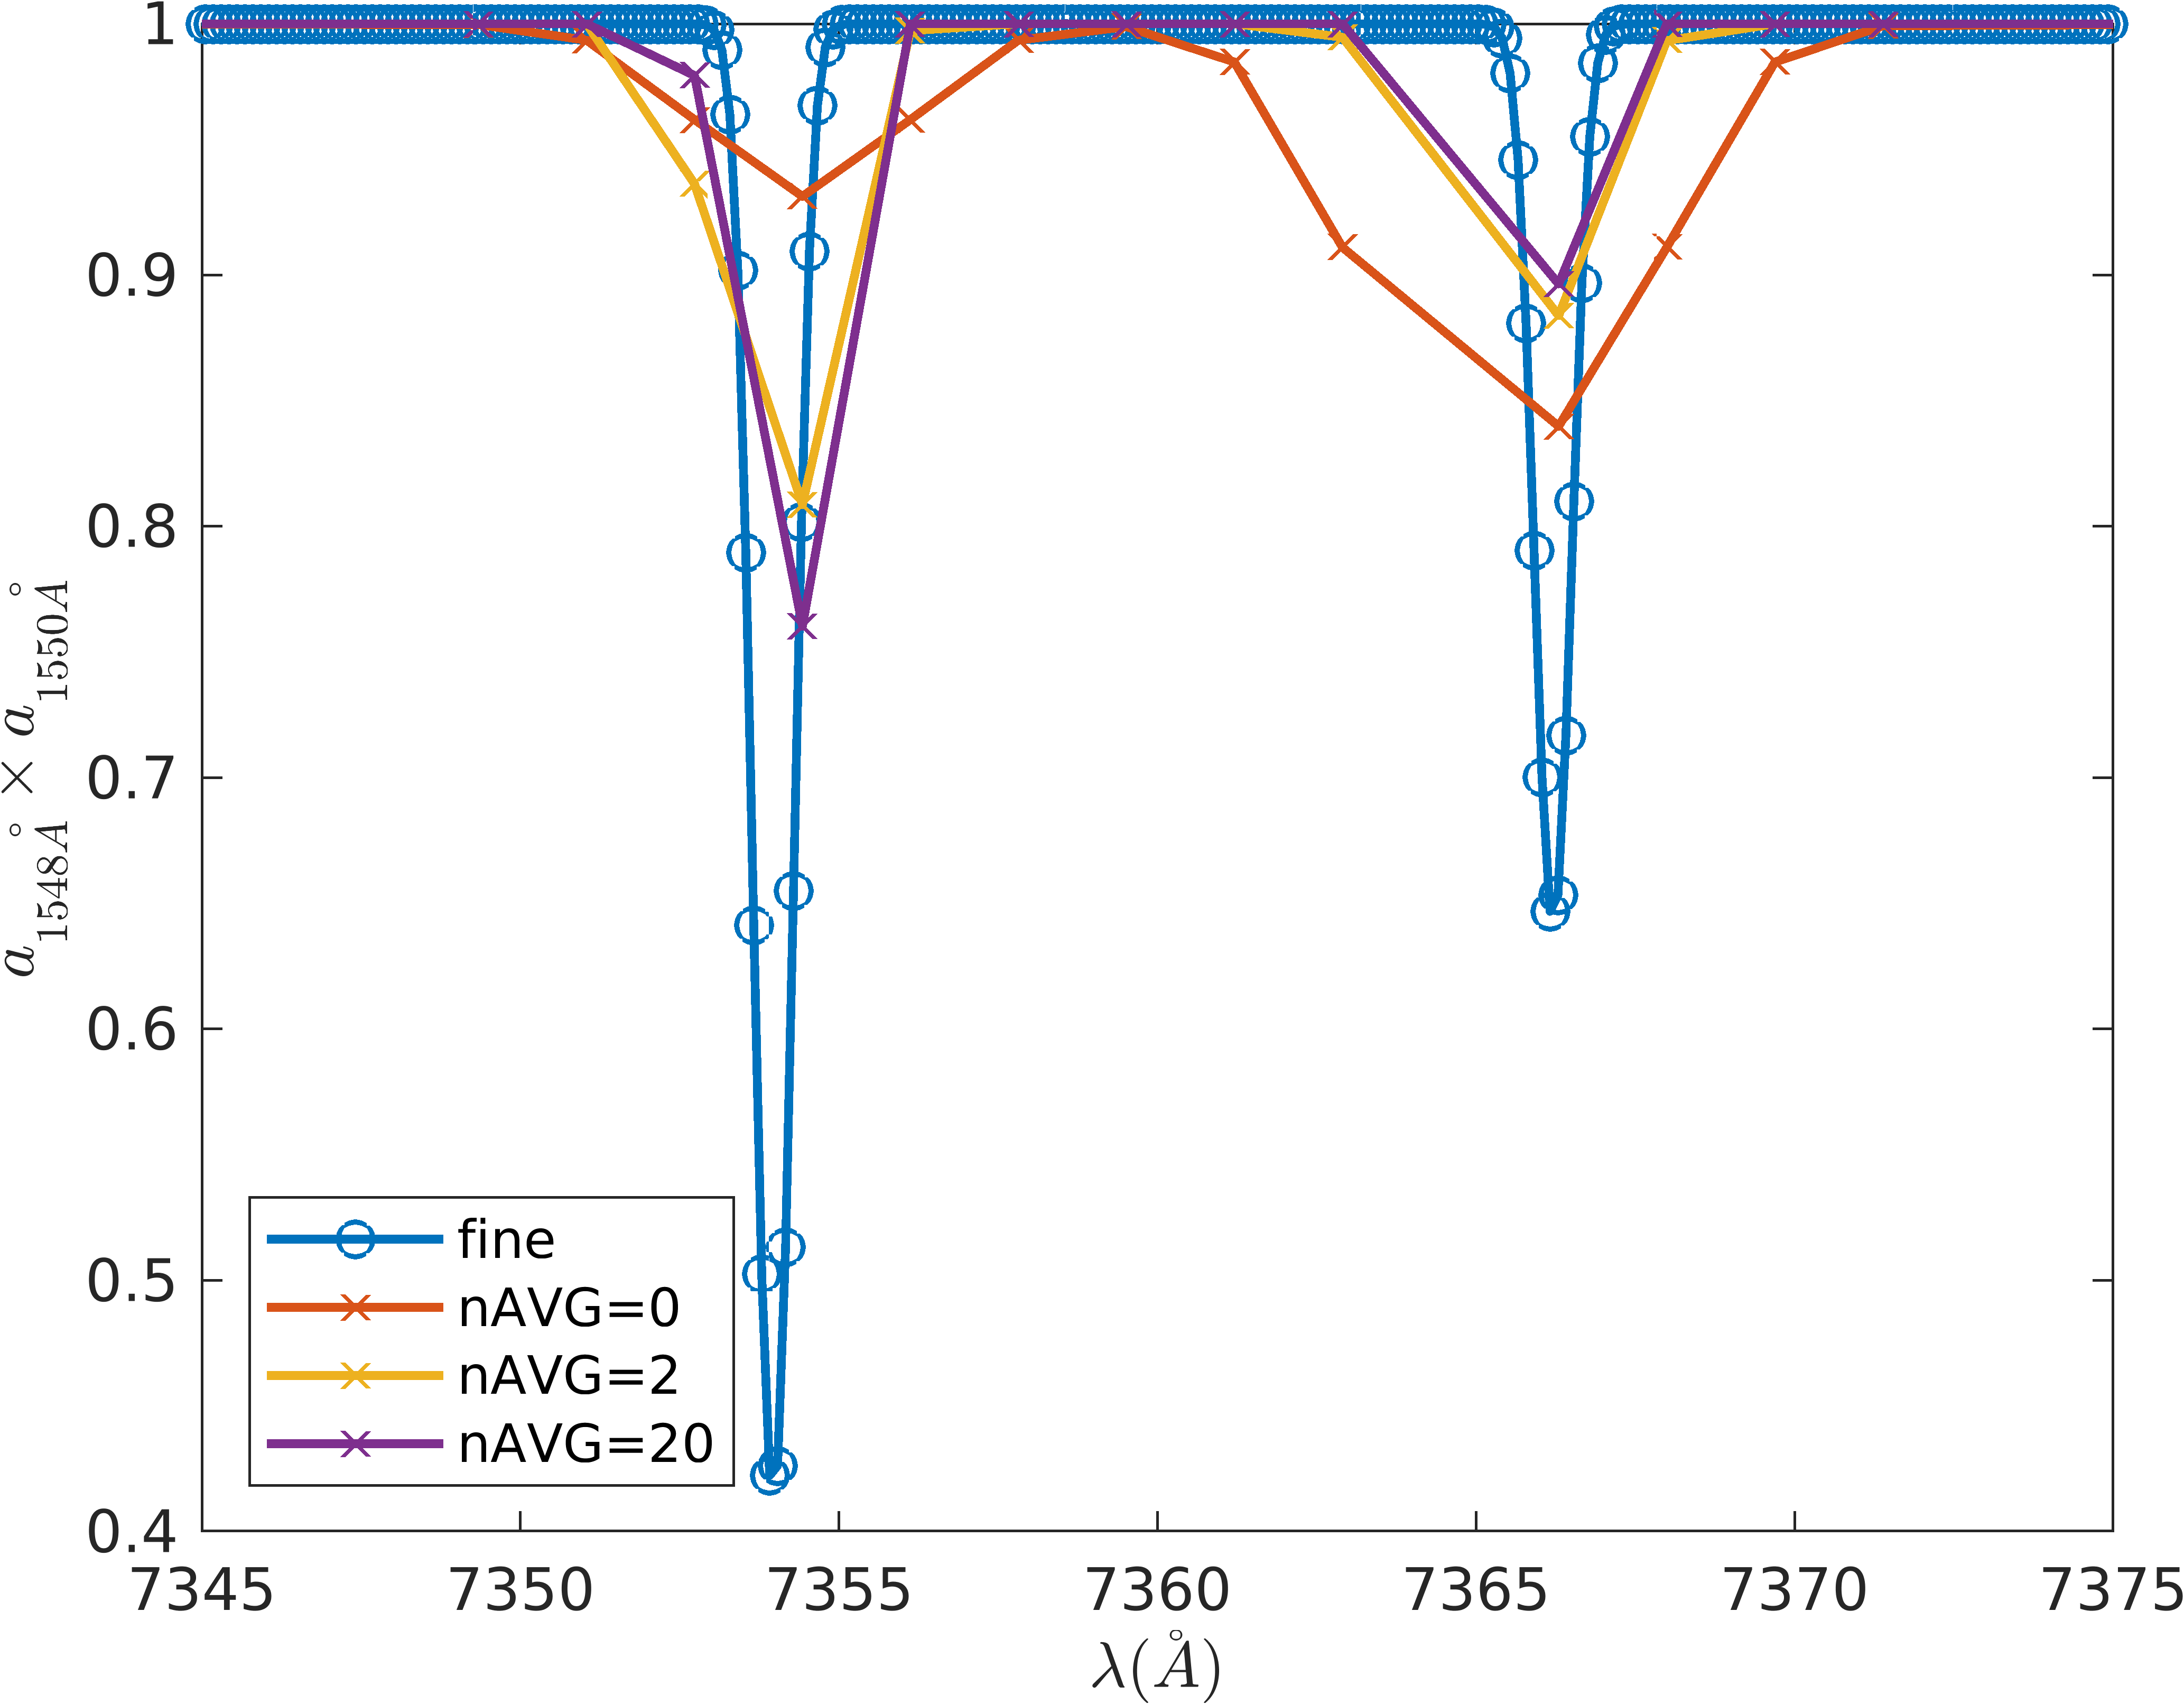
\includegraphics[width=\linewidth]{figs/VoigtTest.png}
  \caption{ Example absorption profile for $\sciv=10$\kms, $\nciv=14.5~cm^{-2}$, and
  $\zciv=1.65$. The blue curve is an absorption profile over a wavelength array with 1000 times
  finer pixel-spacing of SDSS. Other curves show the absorption profile evaluated at the \emph{observed}
  wavelengths of SDSS, but sub-sampled and then averaged using a fine grid of nAVG sub-samples.}
  \label{fig:voigtTest}
\end{figure}

% \spb{Add more details here, as we discussed. Also a sentence about the instrumental broadening profile.}

\section{Validation}
\label{sec:validation}

For validation, we trained a \civ\ free model, $\model_{N}$, on a reduced training set of 95\% of the
inspected spectra in the PM catalogue.
We then \emph{validated} our algorithm with the remaining 5\% of the
inspected (1301) spectra in the PM catalogue to
check the agreement between the catalogue and our method.
Note that when we applied our algorithm to DR12 spectra we re-trained our model
using all spectra, without the 5\% holdout.
% ROC curve
We use the Receiver Operator Characteristic (ROC) curve, which is
 the false positive rate versus true positive rate
 for various classification thresholds.
Our model is compared to the \civ~absorbers as ranked in the PM catalogue. The PM catalogue provides a rough estimate of confidence in an absorber, ranking them as $0,1,2,3$. Absorbers with a ranking $\ge 2$ are considered likely \civ~absorbers by the PM catalogue.
We construct a `ground truth' sample by labelling each spectrum with ranking $\ge2$ as an absorber. For each spectrum we enforce that our detected absorber is within 350 \kms of a detected system in the PM catalogue. The ROC curve in Fig. \ref{fig:ROC} is obtained by computing the number of \civ\ absorbers in our catalogue with posterior probability greater than a threshold.
A higher performance is reflected in a larger area under curve (\textsc{AUC}).
We obtain \textsc{AUC}$=0.862$, which is quite reasonable.

\begin{figure}
  \centering
  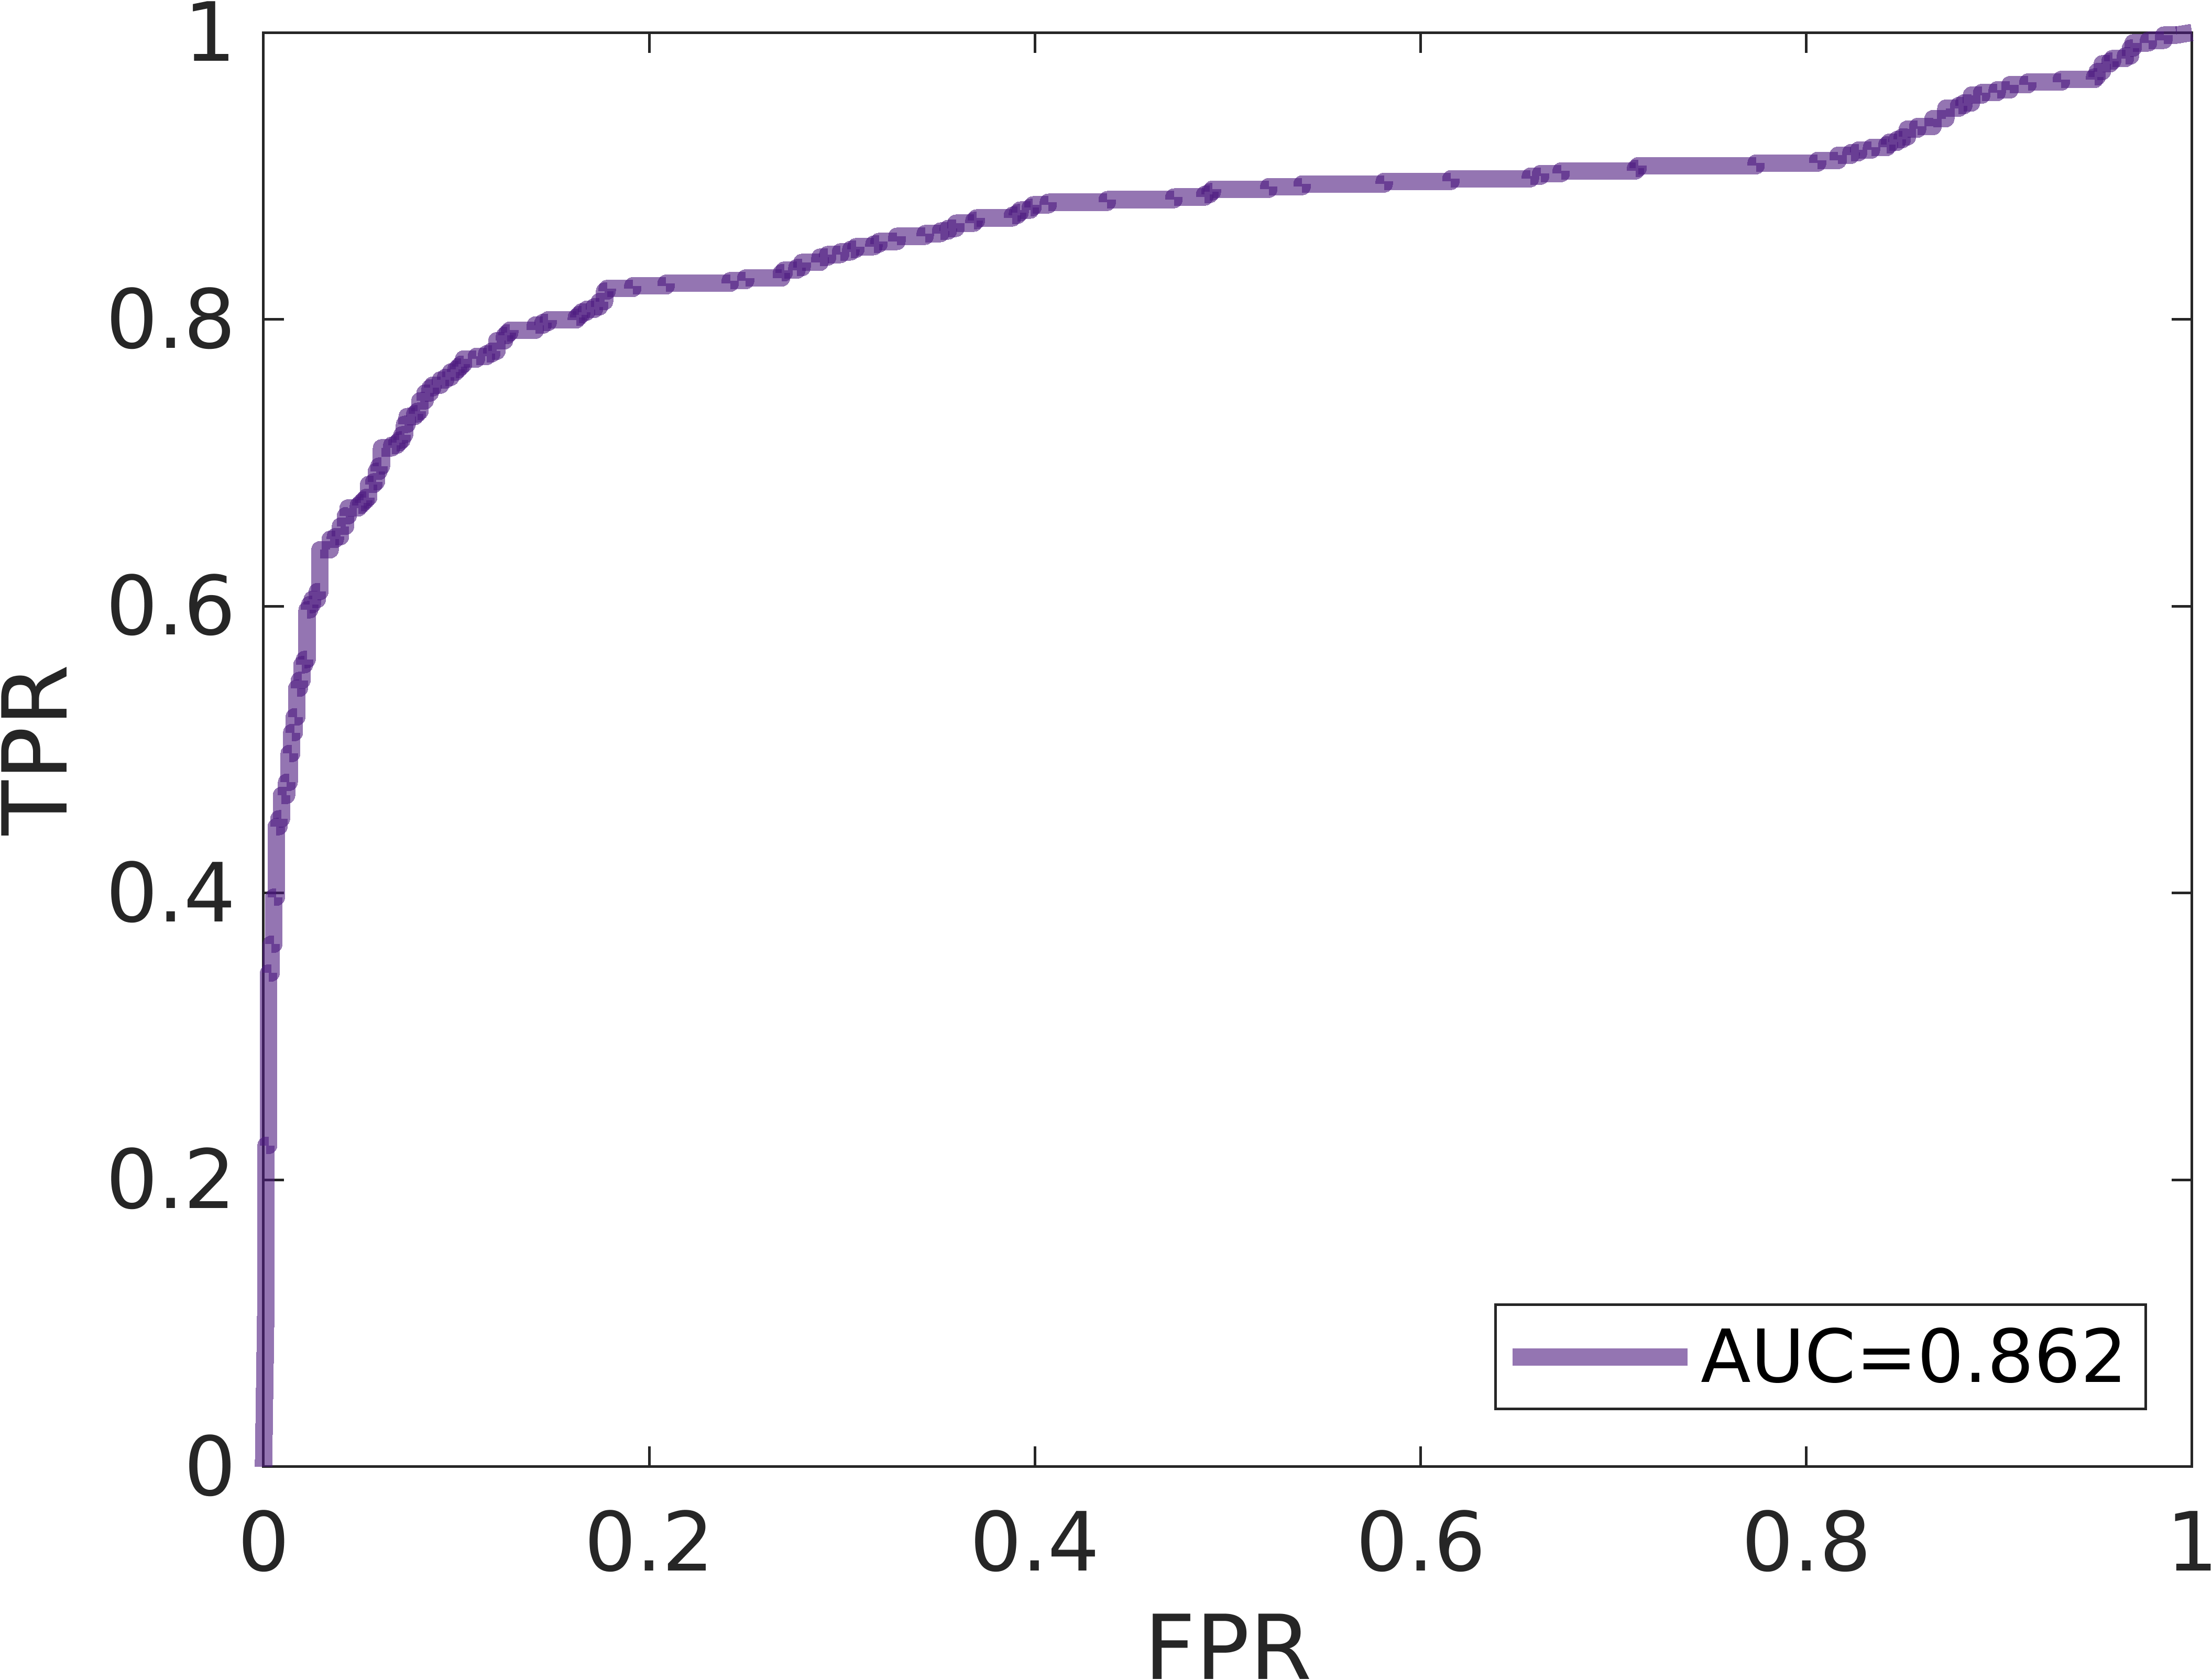
\includegraphics[width=\linewidth]{figs/ROC-N-1250-1610-S-35-115-NoOcc-nc-10k-vf.png}
  \caption{Receiver Operator Characteristic (ROC) curve for our DR7 validation. True Positive Rate (TPR) is plotted versus False Positive Rate (FPR). The area under the ROC curve (AUC), a measure of the validity of classification, is 0.854.
  %An ideal classification gives an AUC of 1.
  }
  \label{fig:ROC}
\end{figure}

We also assessed performance by comparing individual absorption systems. We can compare our GP catalogue for various \civ\ posterior probabilities to the `ground truth' sample of the PM catalogue.
%a catalogue of absorbers with ranking $\ge2$ in the PM catalogue. We define absorbers as being the same when their redshifts are less than $350$ \kms apart.
We define the purity of our GP catalogue as the fraction of the GP catalogue also in the PM catalogue:
\begin{equation}
\mathrm{Purity} = \frac{\mathrm{GP\; and \;PM}}{\mathrm{GP}}.
\end{equation}
The completeness is the fraction of the PM catalogue also in the GP catalogue:
\begin{equation}
\mathrm{Completeness} = \frac{\mathrm{GP \;and \;PM}}{\mathrm{PM}}.
\end{equation}
These definitions understate the agreement between the two methods as there is no correction for inherent sensitivity. Each technique will have a different threshold at which it can detect weak absorbers. Thus a difference in the catalogues may occur which is not due to spurious absorbers, but simply absorbers beneath the sensitivity threshold of the other technique. We shall see that the GP catalogue turns out to be slightly more sensitive than the PM catalogue, reducing the apparent purity.

Fig. \ref{fig:threshold} shows completeness and purity as a function of threshold value.
One should choose a threshold that gives the best possible
combination of purity and completeness, around the point where the curves intersect.
We thus choose a threshold of 95\%, which Fig.~\ref{fig:threshold} shows produces purity and completeness of $\sim 80\%$ in a roughly equal balance.
However, our catalogue reports posterior probabilities, so the user may choose a different threshold as desired for their application. One may sacrifice purity for completeness or vice versa.

\begin{figure}
  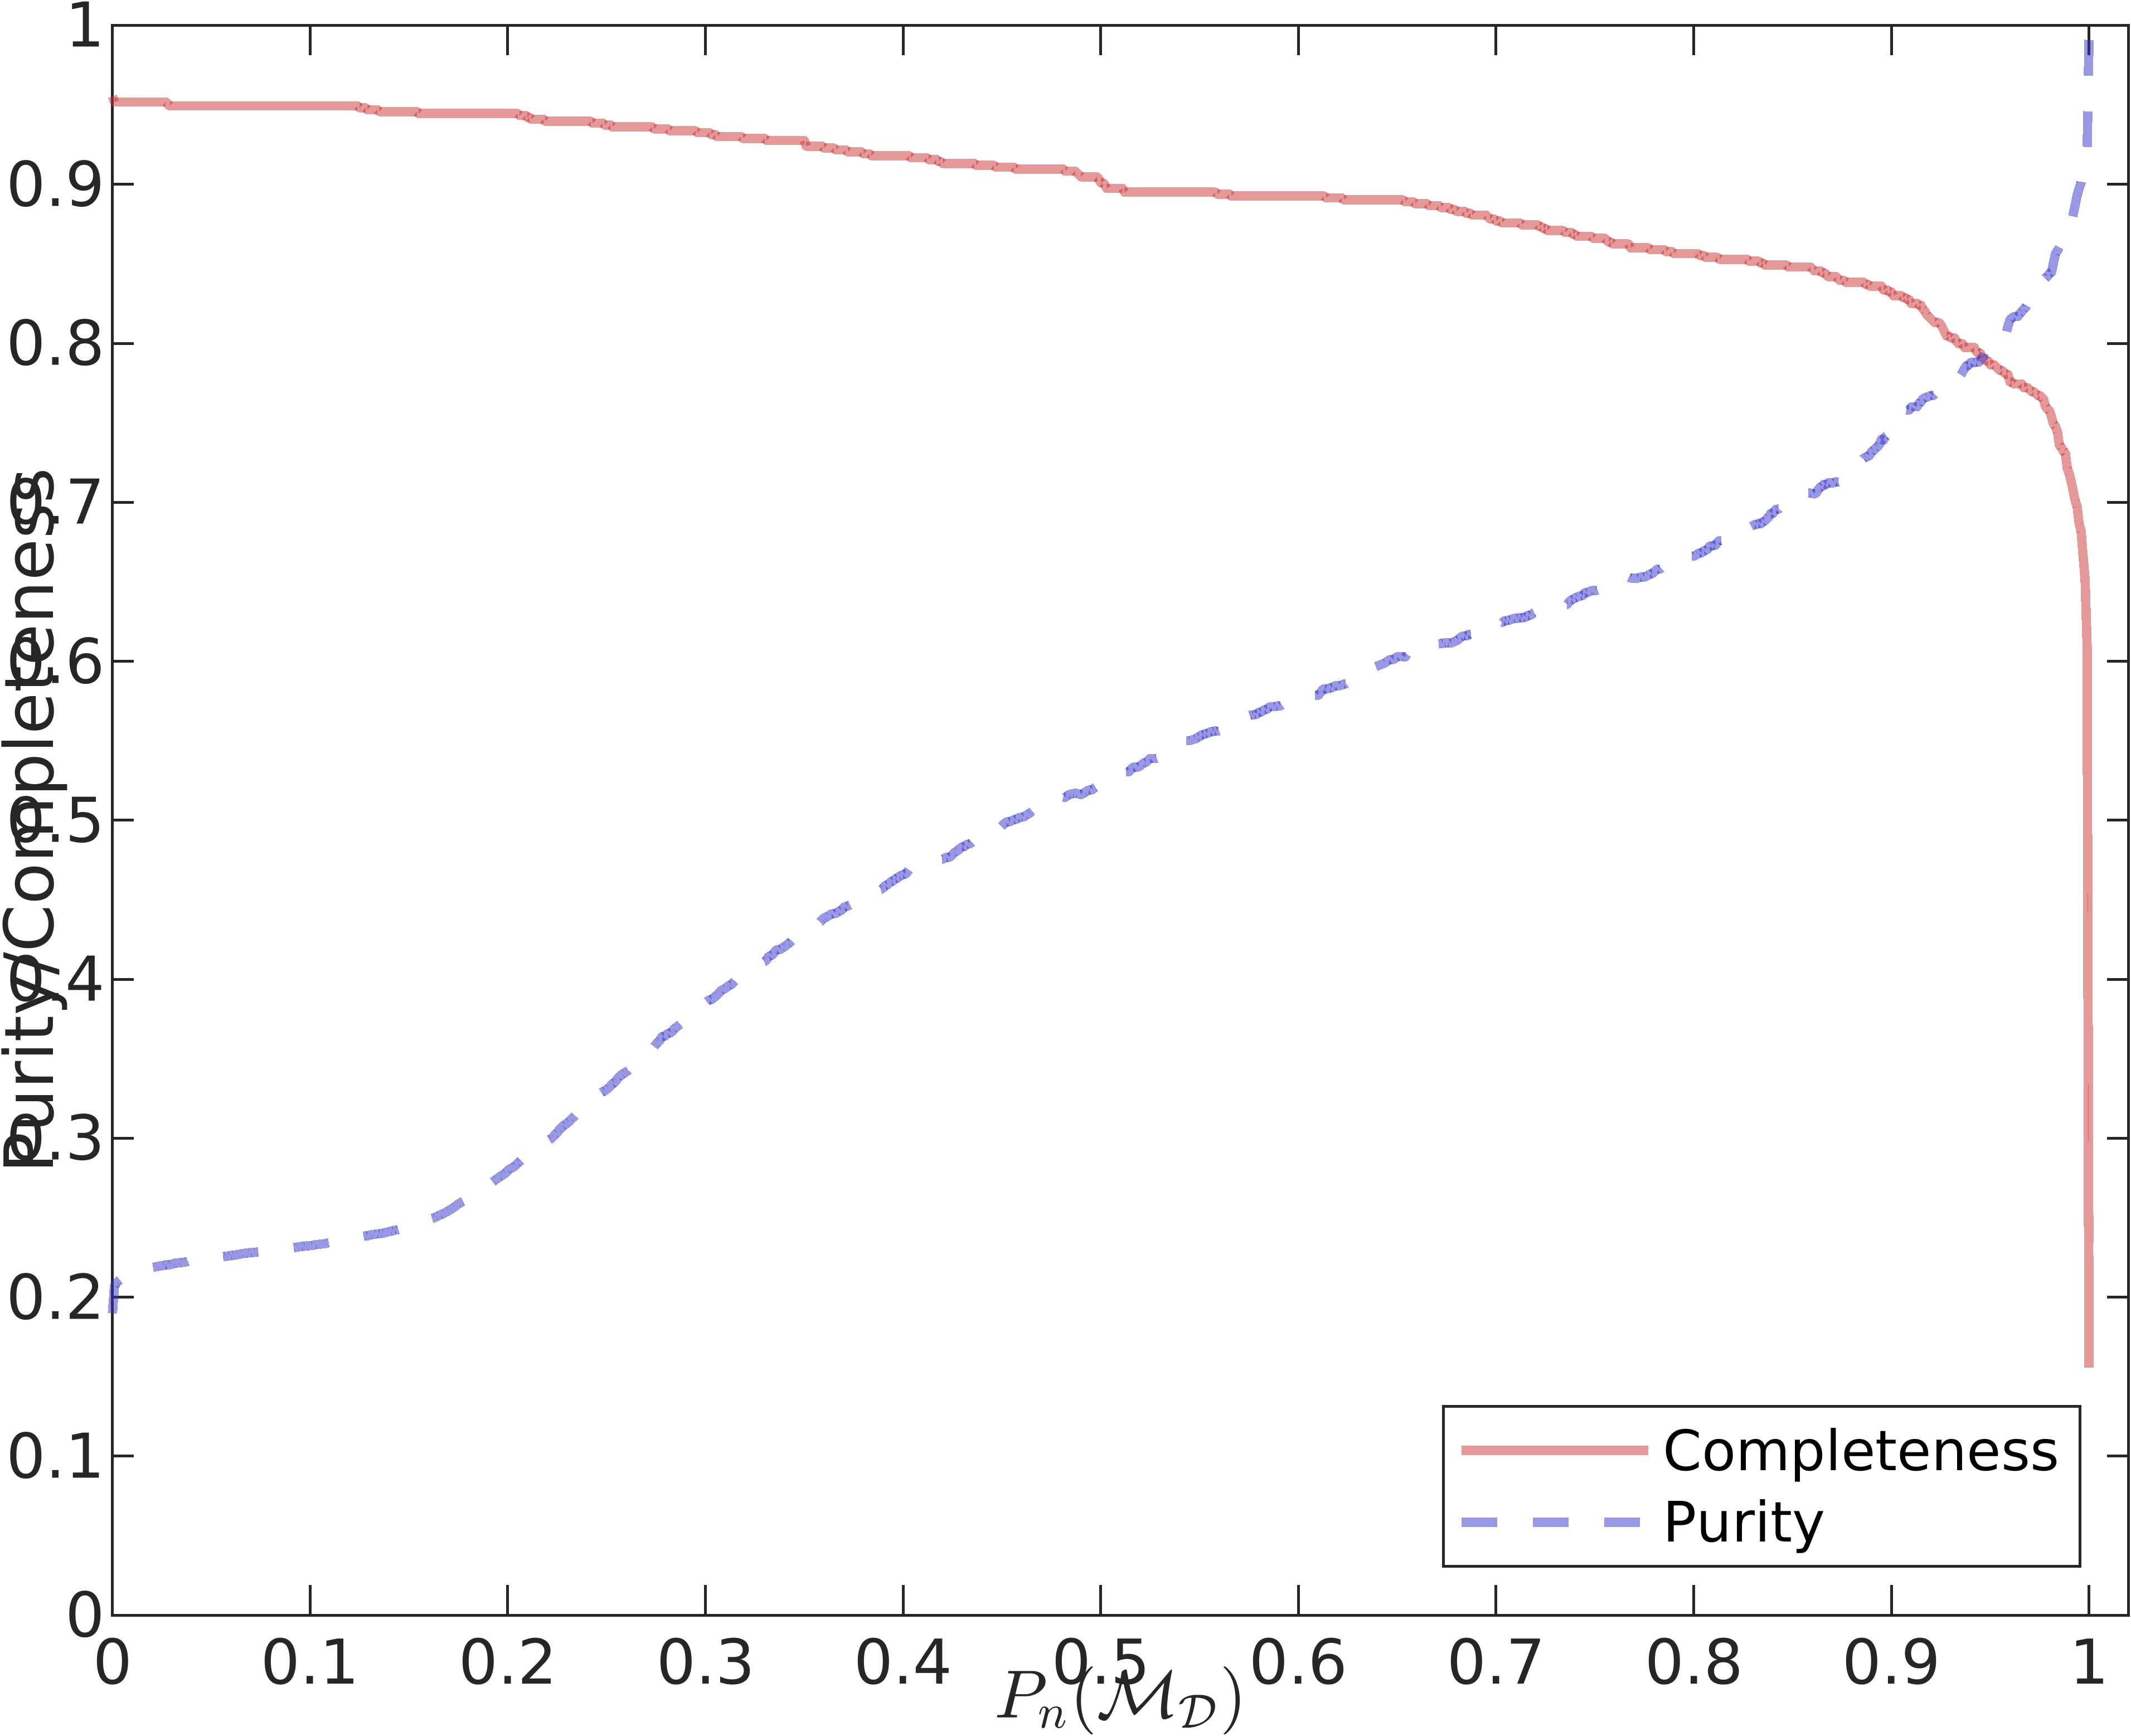
\includegraphics[width=\linewidth]{figs/PC-N-1250-1610-S-35-115-NoOcc-nc-10k-VoigtFixed.png}
  \caption{Purity and completeness of the GP catalogue compared to the PM catalogue for different \civ\ posterior probability thresholds.
  The maximum allowed velocity separation between our catalogue and the PM catalogue absorbers is 350 \kms.}
  \label{fig:threshold}
\end{figure}

Fig.~\ref{fig:Dewdr7} shows the difference ratio in our validation set between REW from the PM catalogue and REW from integrating the MAP Voigt profile in the GP catalogue:
\begin{equation}
\mathcal{R}_\mathrm{REW} = 1-\frac{REW_{PM}(1548A)}{REW_{GP}^{Voigt}(1548A)}
 \end{equation}
The bulk of the distribution for $\mathcal{R}_\mathrm{REW}$ lies between
    $\pm50\%$, which shows a reasonable consistency between the GP and PM catalogues.
    We visually inspected the spectra of absorbers where $\mathcal{R}_\mathrm{REW}$ was large.
    There are $16$ absorbers with $P_\mathrm{CIV} > 0.85$ that have $\mathcal{R}_\mathrm{REW} < -1.5$. Four absorbers out of 16 are located at the very blue edge of the observed band. Eight are from very noisy spectra and have unusual continua shapes. The remaining two are very strong absorption close to the quasar, potentially undetected mini-BALs or heavily blended \civ\ absorbers.
    The REW in the PM catalogue is not computed by Voigt fitting, but by boxcar integration of the flux
     $5\sciv$ (in velocity units) around the detected \civ\ absorber. We checked using a similar routine and found similar levels of agreement between PM and our Voigt fitting. As we did not attempt to divide out the continuum with this method the agreement between the two catalogues was moderately worse.

    %  \spb{Not sure we need the below, maybe remove: This comparison implies that
    % the REW(1548\AA) that we find from direct integration of Voigt profiles in Eq.
    % \ref{eq:rewgp} can be some times smaller than REW values
    %  we find from pixel-wise boxcar summation of flux through the
    % absorption region, 350 \kms around the found absorber. That is reasonable because
    % Voigt profile is less sensitive to noisy pixels and the boxcar summation can
    % overestimate the REW at some cases. We can use this criteria as a sanity check for our searched
    % systems, that is when the difference between REW from boxcar summation is off by more than
    % twice the estimated error coming from pixel noise, we can ignore the found absorber. Also
    % another sanity check with boxcar summation REW is that sometimes due to a strange or noisy
    % continuum we may get a negative REW which clearly points to a not reliable absorber system.}


    % \rmon{What about checking balnicity index and it is more 500 then we remove it in
    % post-processing.} \spb{Good idea to check! Don't think any need to remove it though.}
    \begin{figure}
      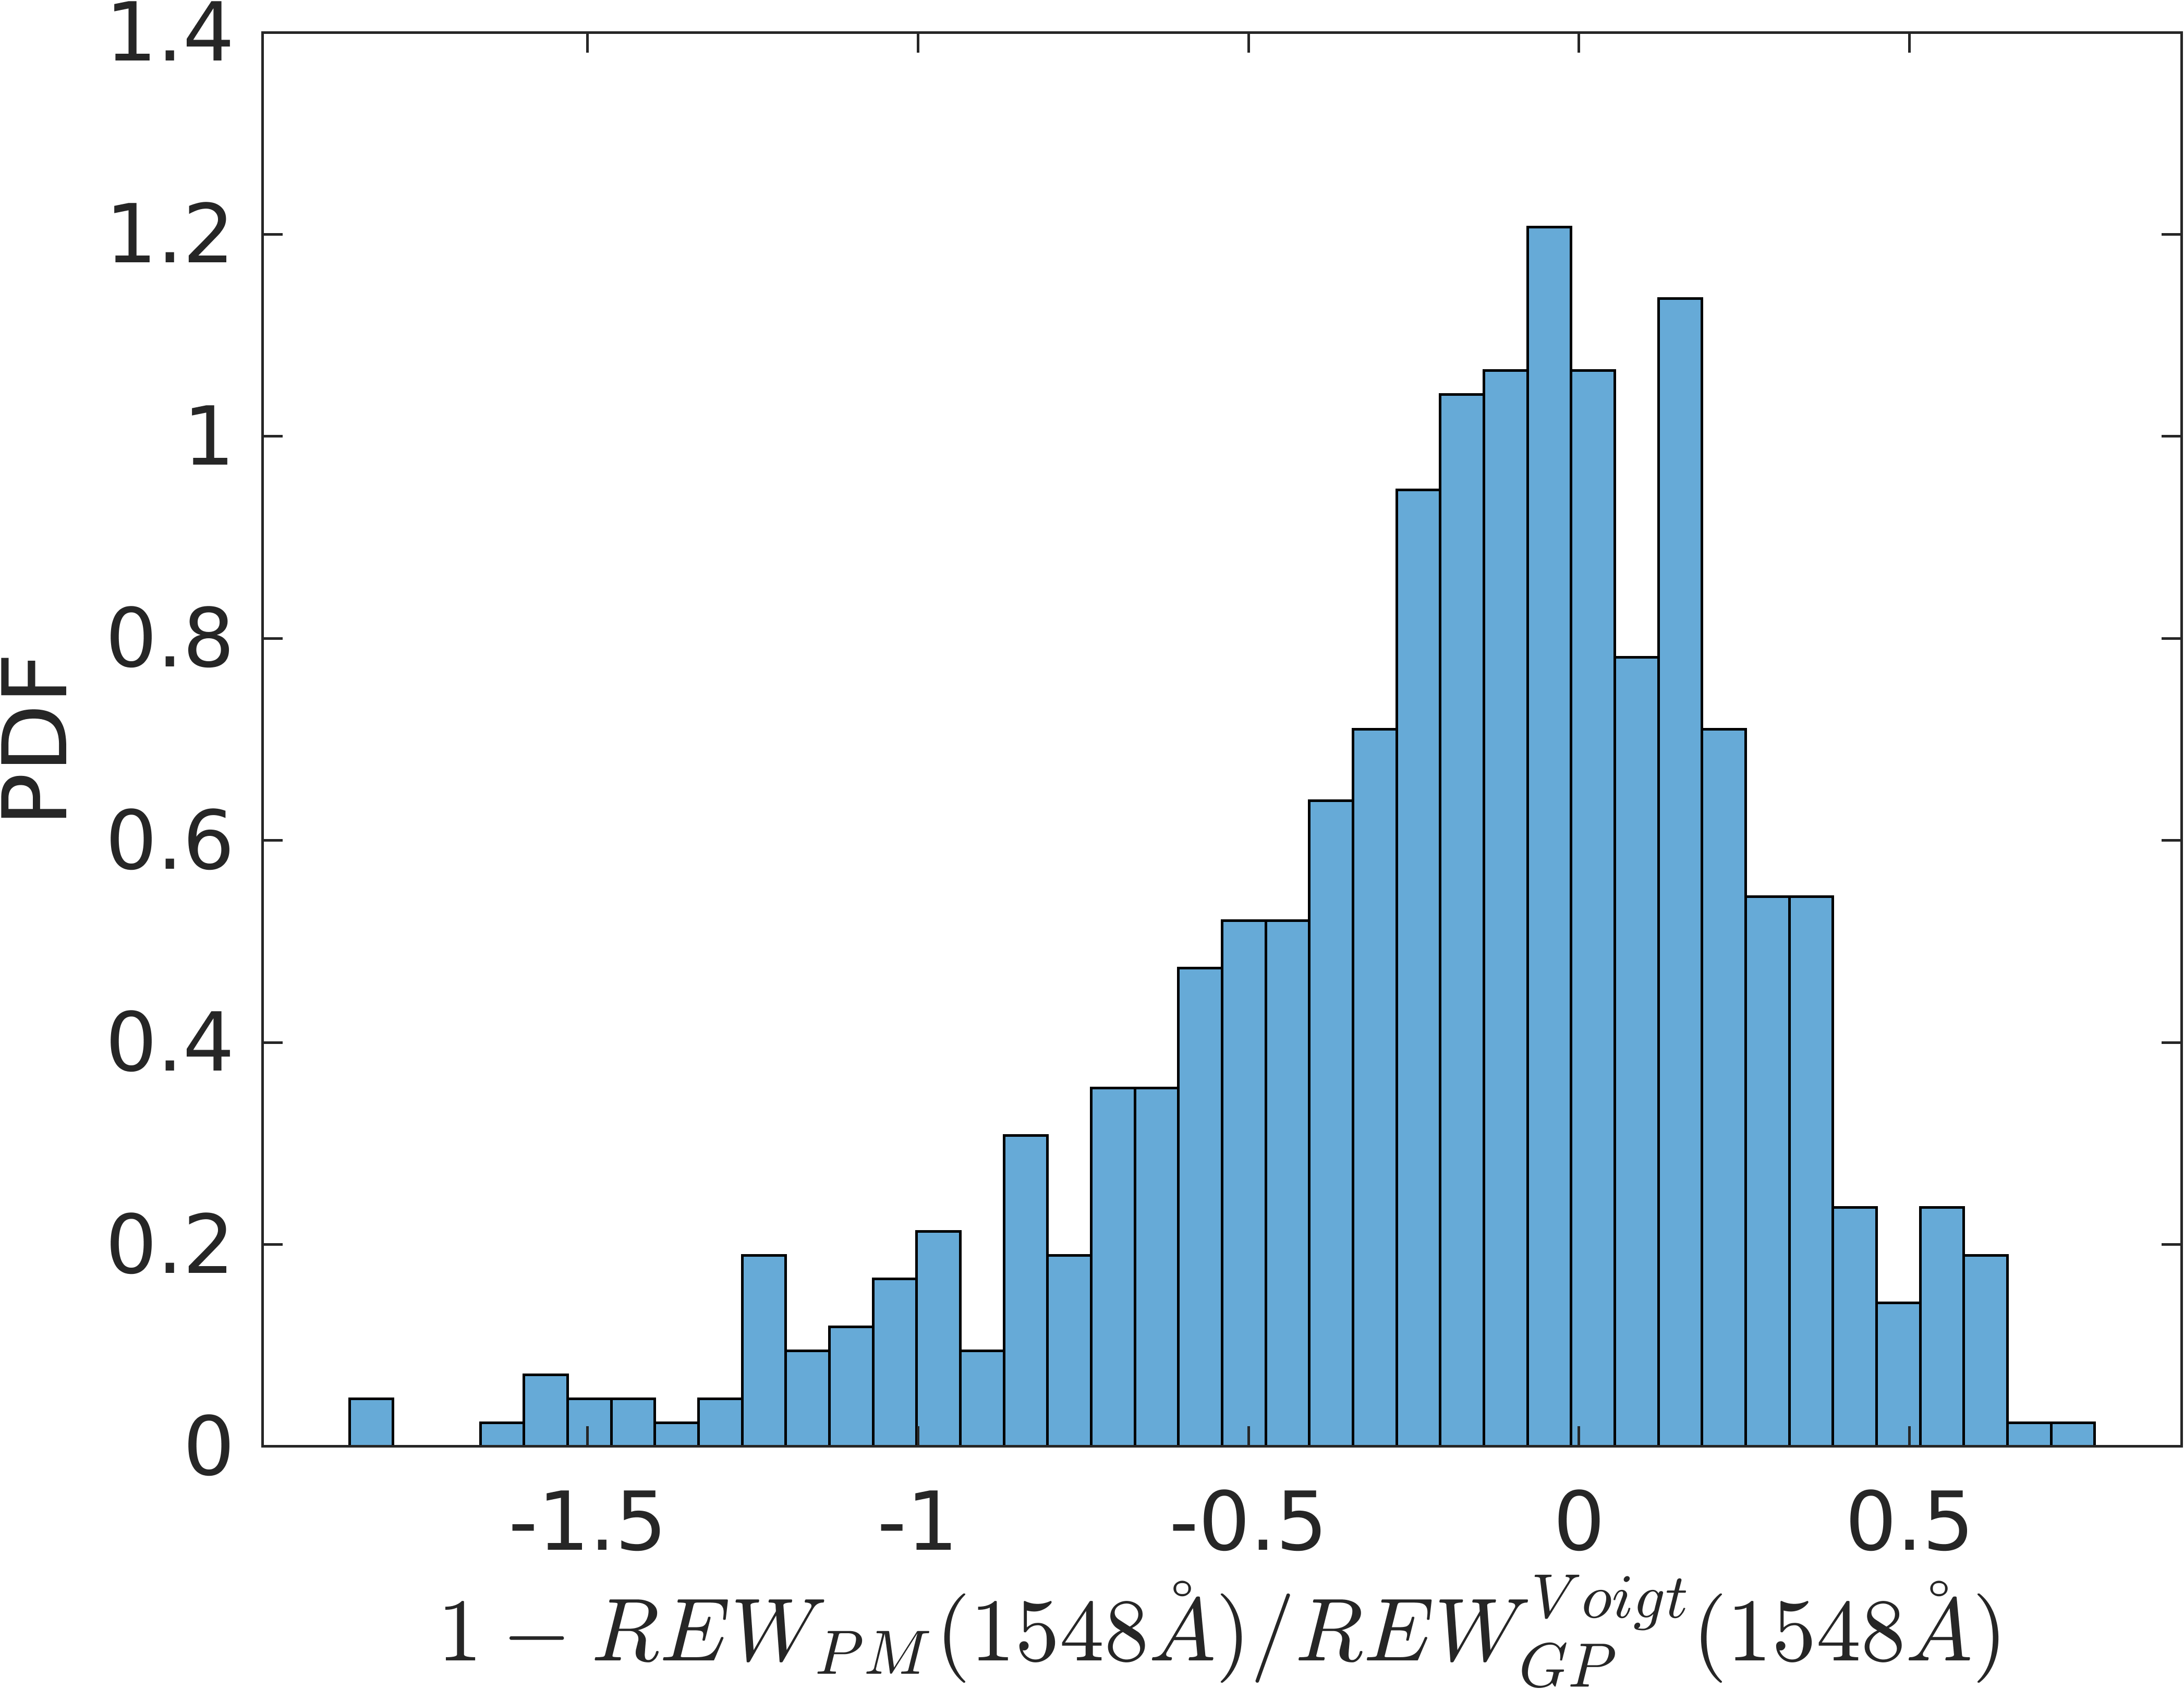
\includegraphics[width=\linewidth]{figs/dEW-voigt-nc10k.png}
      \caption{The ratio between the rest
      equivalent widths of the 1548\AA~line for \civ~absorbers in our validation set, detected in both the PM catalogue and the GP catalogue. %8 out of 16 absorbers with a ratio $< -1.5$
      %have very noisy quasar spectra and an oddly shaped continuum.
      %4 out of 16 of them are located at the very blue end of the spectrum, where SDSS data is noisy.
      }
      \label{fig:Dewdr7}
    \end{figure}



%     We looked at the distribution of column density sigma parameter of all absorbers
%     within iur validation set that we found a probability larger than 85\% for being a
%     legit \civ\ absorber (GP1) and compared it with those that both GP method and  PM-catalogue
%     agree about them (PM1GP1). Fig. \ref{fig:pm1gp1} shows most of the absorbers which both PM-catalogue anf GP-catalogue agree upon have
%     large sigma parameters and have column densities larger than $10^{14} cm^{-2}$. This
%     large range of estimated $\sciv$ values for indicates that our found systems are not single/isolated
%     systems, but we are detecting a complex system of absorbers which are closer to each other
%     than the resolution of SDSS spectra which is roughly 150 \kms.
% \begin{figure}
%   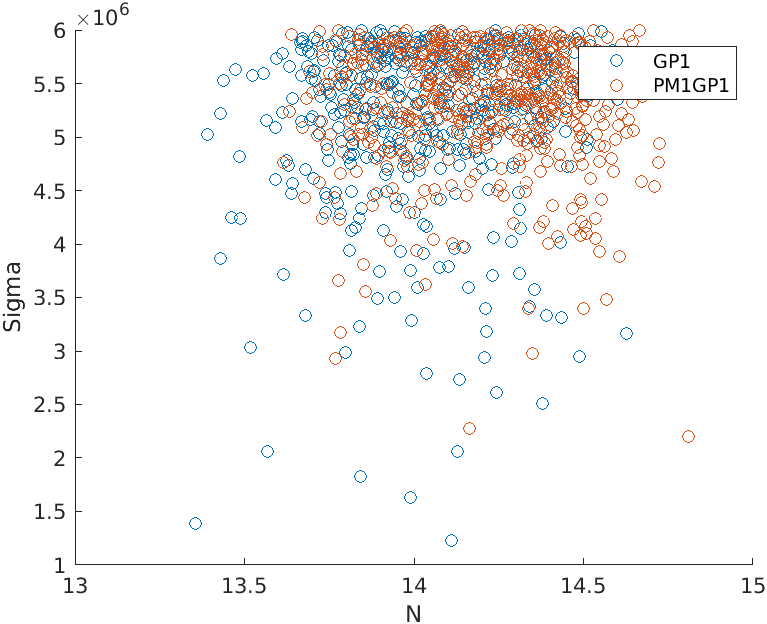
\includegraphics[width=\linewidth]{figs/N-Sigma-PM1GP1-GP1.png}
%   \caption{The distribution for column densities
%   and sigma parameters in GP1 and PM1GP1 samples.}
%   \label{fig:pm1gp1}
% \end{figure}

The velocity separation between absorbers detected in both the GP and PM catalogues is shown in
Fig. \ref{fig:dz}. Velocities are consistent at the level of SDSS velocity
resolution. The GP pipeline velocity produces slightly redder \civ~absorbers than the PM catalogue, with a median offset $\Delta \zciv < 50$ km/s. The reason potentially is ... \rmon{We need Kathy's comments here}.
\begin{figure}
  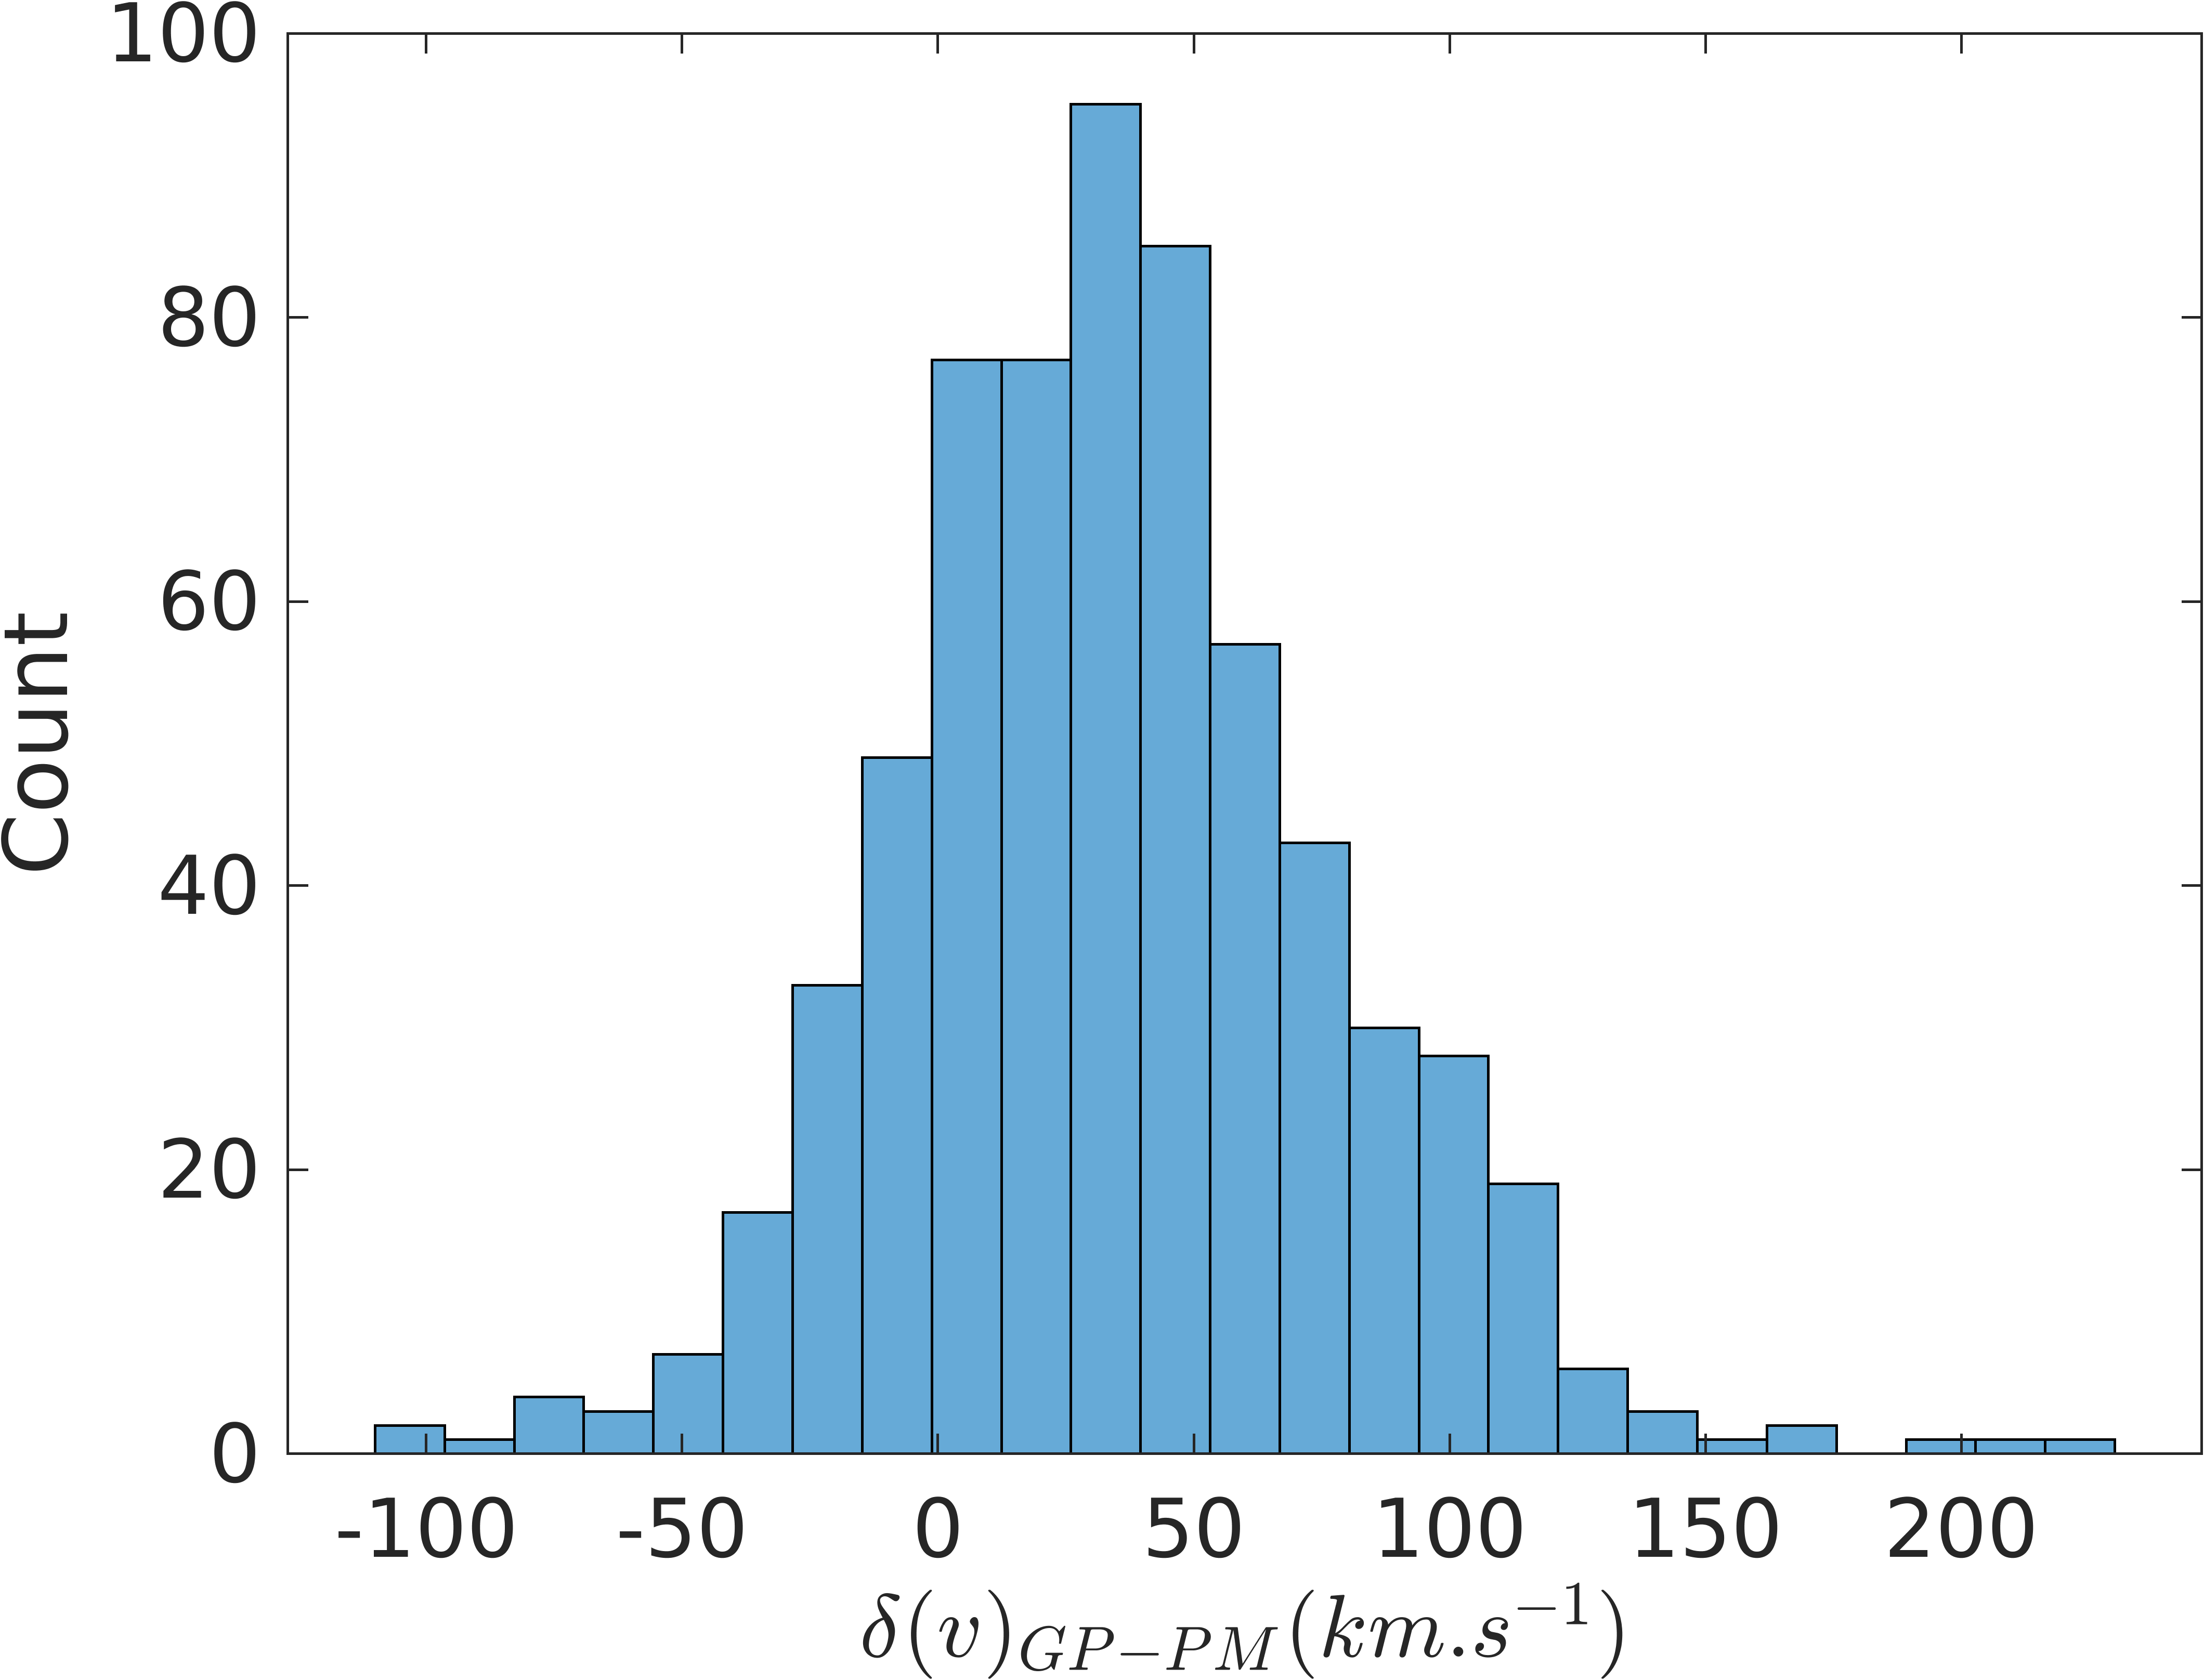
\includegraphics[width = \linewidth]{figs/dvrdz-nc10k-VoigtFixed.png}
  \caption{Velocity difference between  the detected absorbers in
  GP with $P_n(\model_D)\ge0.95$ and the PM catalogue. Only matching absorbers whose velocity difference is closer than 350\kms are shown. }
  %to an absorber in
  %PM catalog with rating $\ge 2$.}}
  \label{fig:dz}
\end{figure}

Fig. \ref{fig:REWDR12} shows the distribution of rest equivalent widths for absorbers in the GP catalogue but absent in the PM catalogue.
These absorbers had preferentially slightly lower REW, suggesting that the sensitivity of our method to weak absorption is slightly higher than the PM catalogue. The purity shown in Fig.~\ref{fig:threshold} may thus understate the purity of our catalogue as some of our newly found absorbers may be real but simply missed by the PM catalogue.

\begin{figure}
  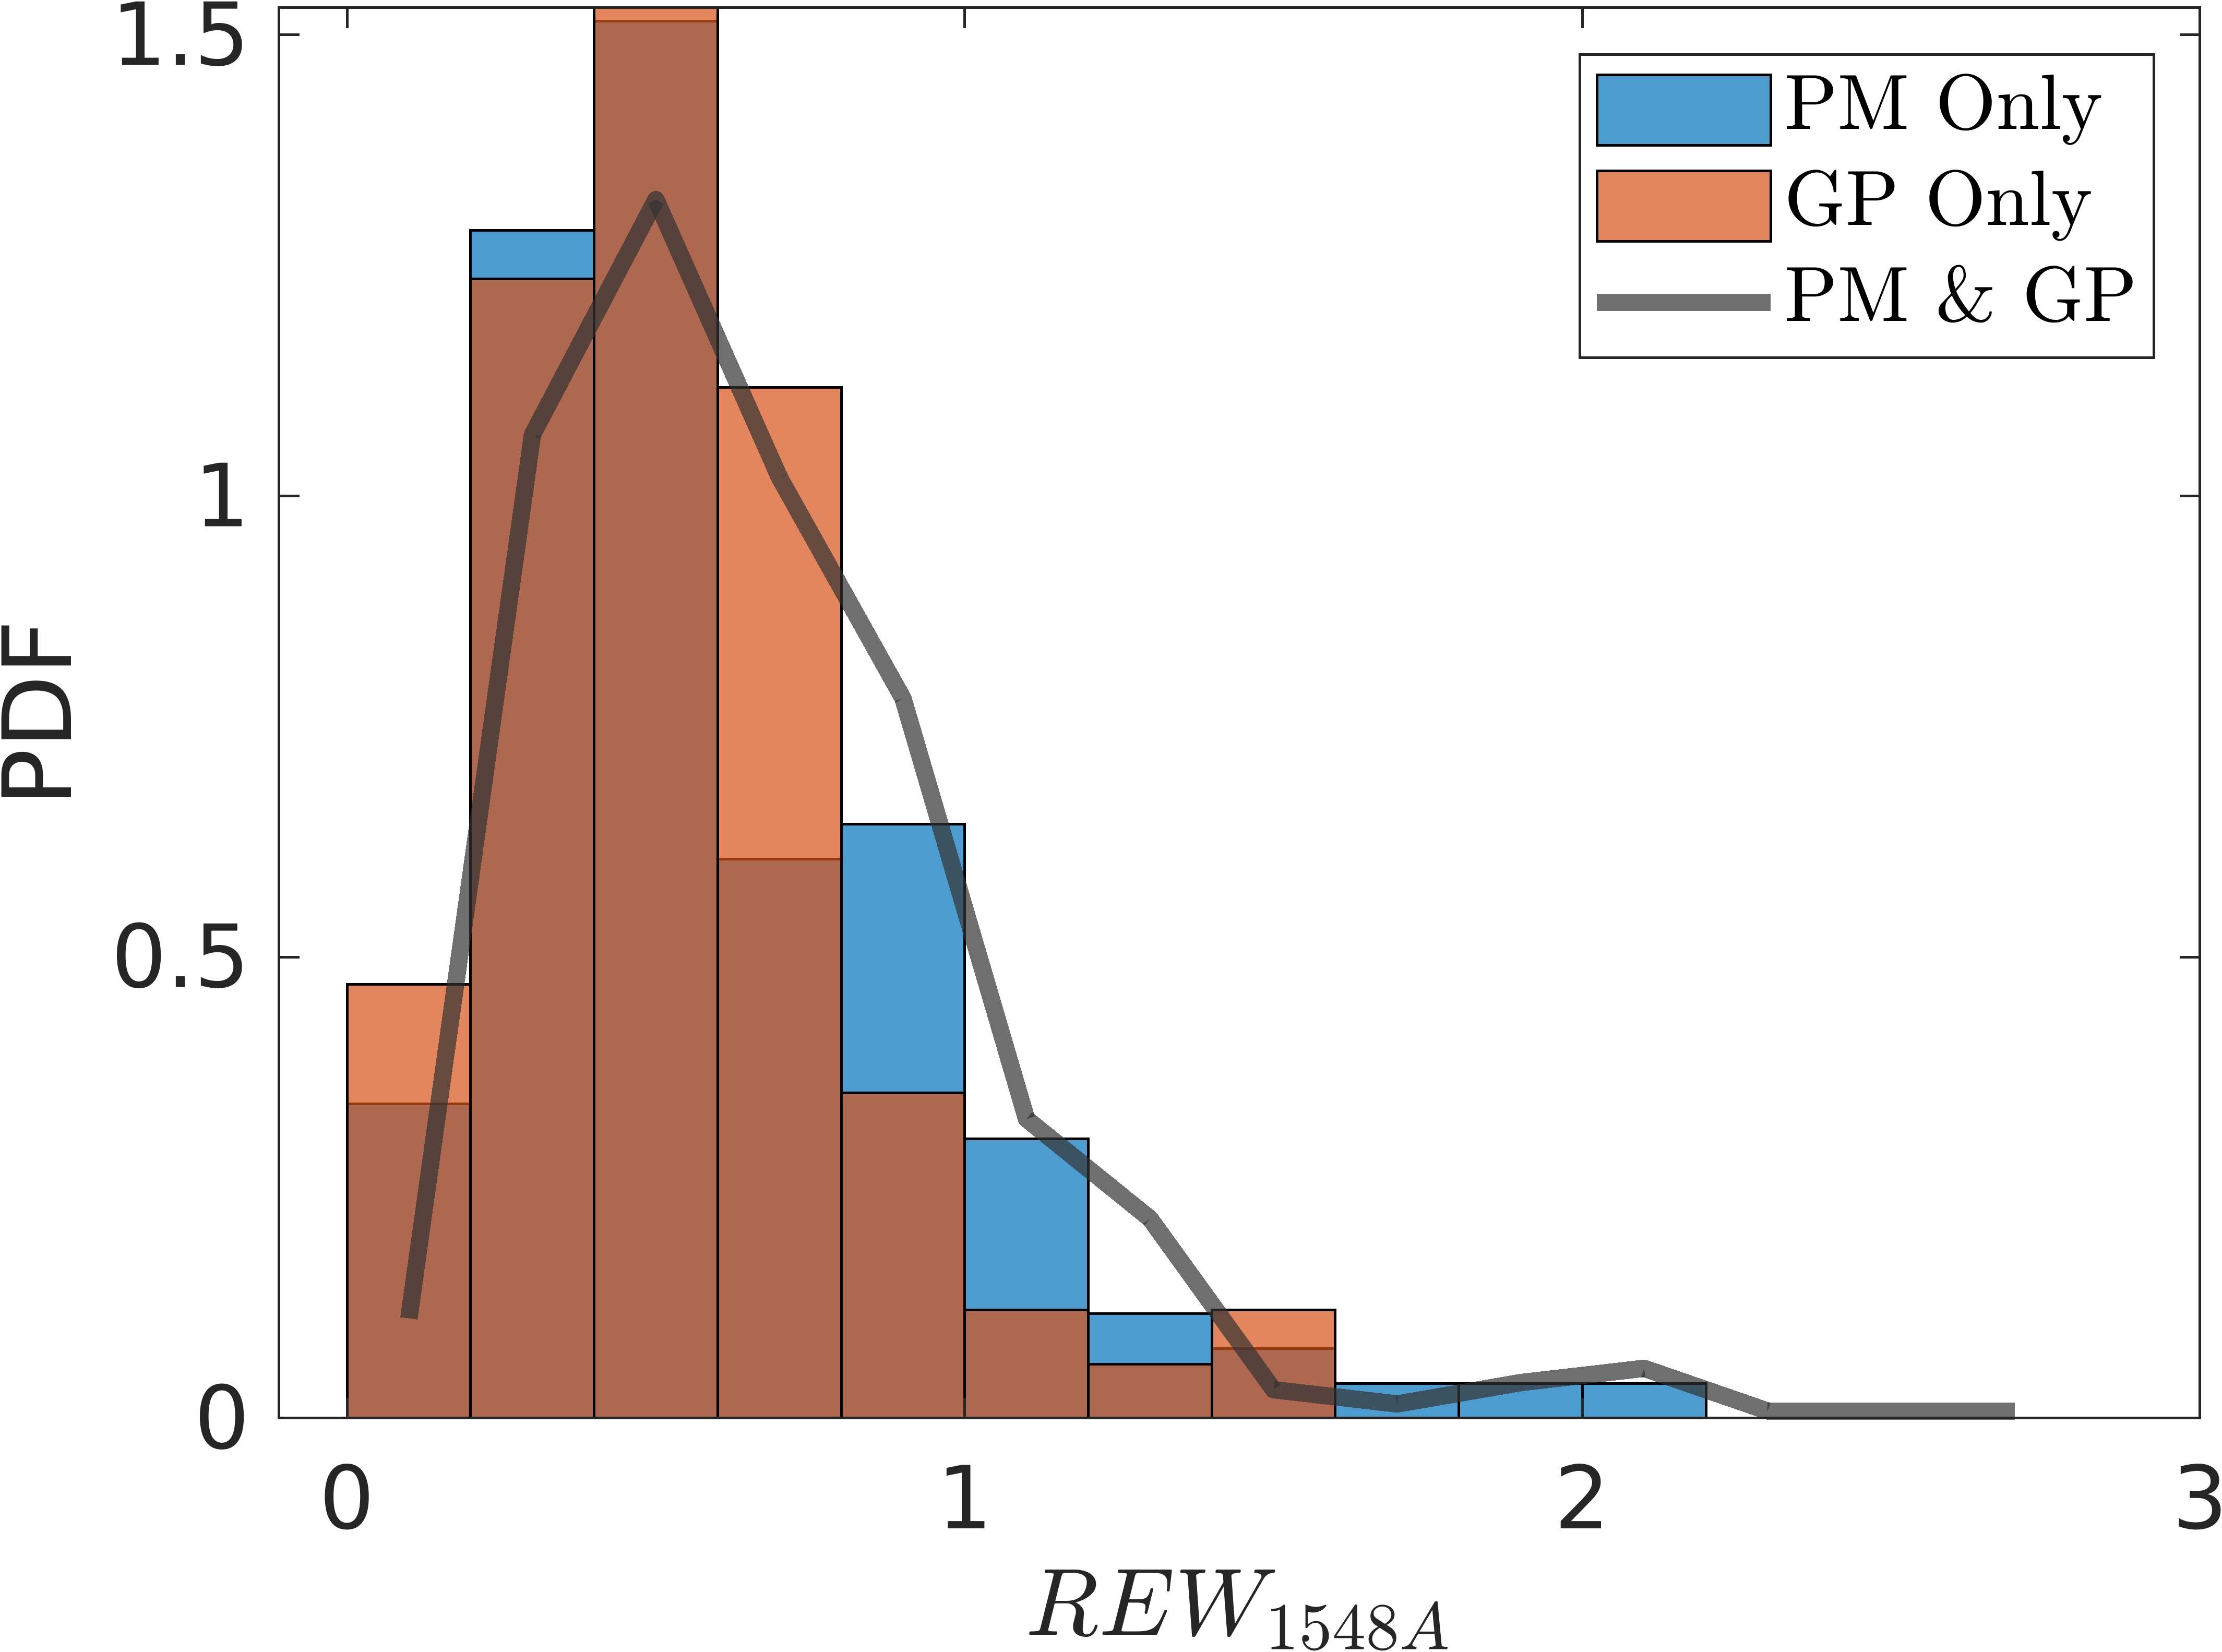
\includegraphics[width=\linewidth]{figs/REW_GP_PM_P95.png}
  % 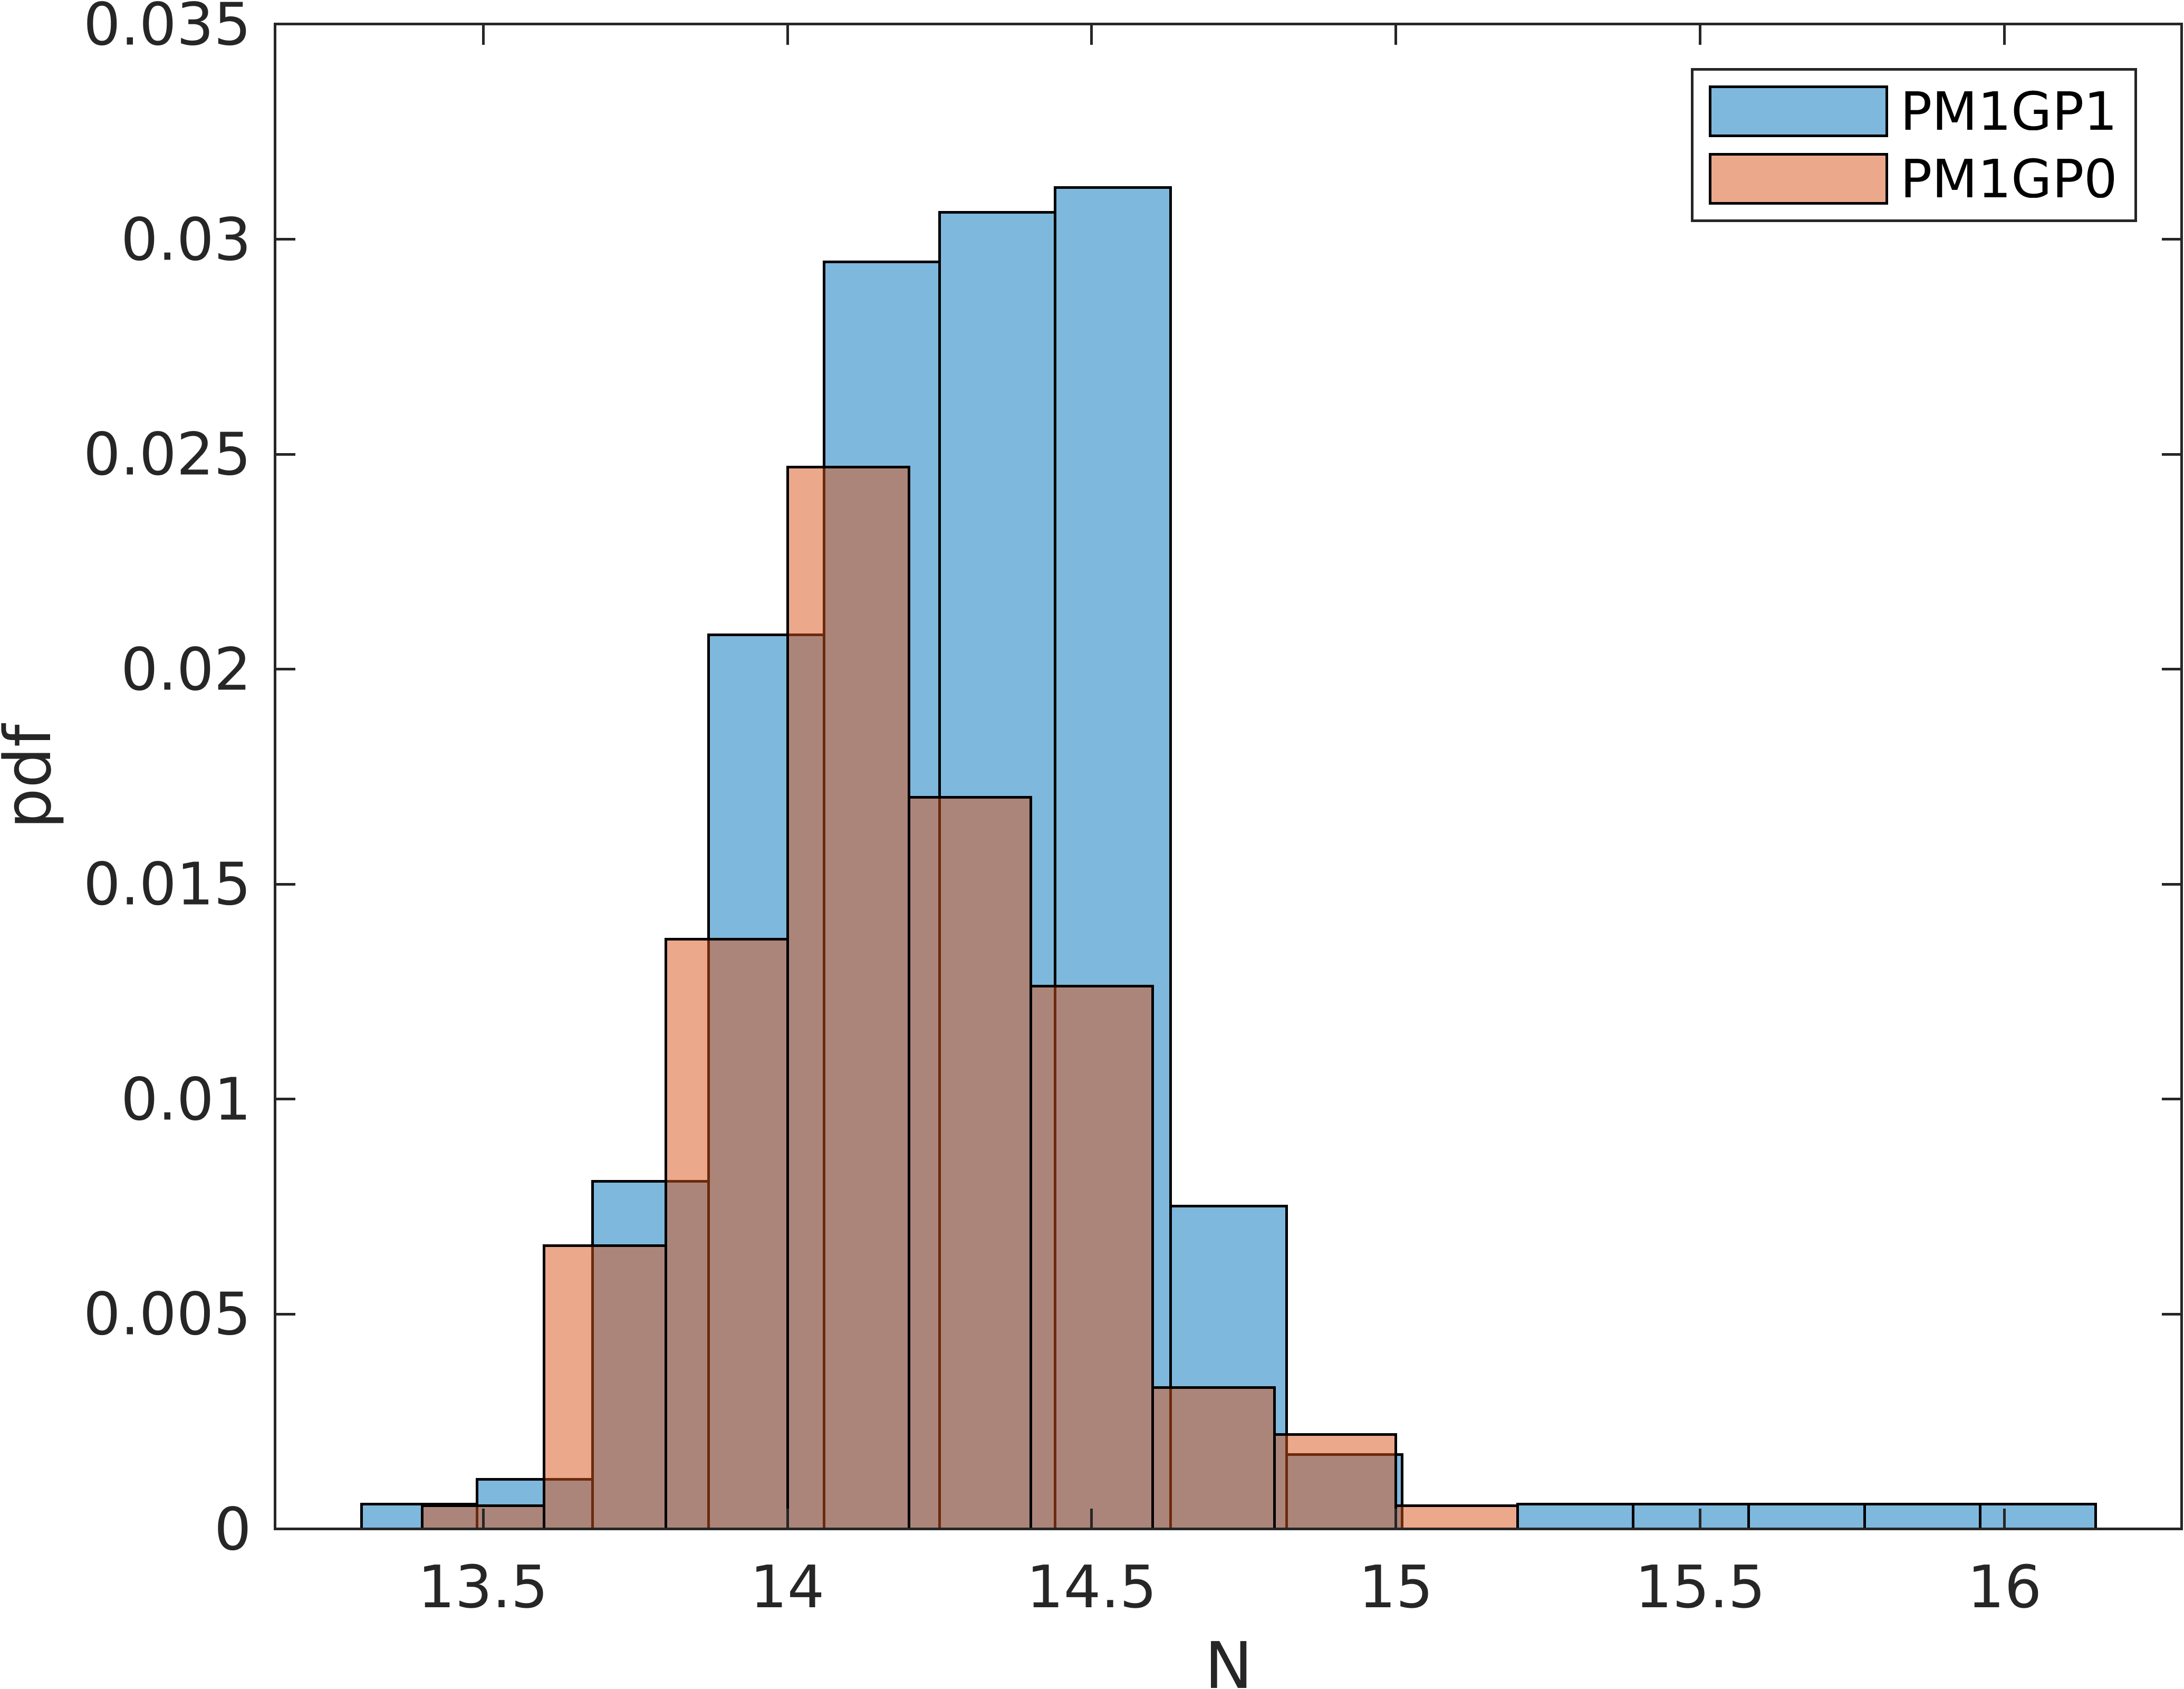
\includegraphics[width=\linewidth]{figs/N-PM1GP1-PM0GP1.png}
  \caption{Distribution of REW for 1548\AA~line for absorbers detected in both the GP and PM catalogues (thick black line), in the GP catalogue only (blue) and in the PM catalogue only (red).
  % Lower panel: Same as upper panel but showing column densities.
  }
  \label{fig:REWDR12}
\end{figure}

% PM1GP1 PM0GP1
Fig. \ref{fig:PM1GP0} shows an example spectrum where the GP catalogue
is missing absorption already detected in the PM catalogue. We investigated some of
the spectra in this category. Many of them in fact had \civ\ detection in both
catalogues, but with a velocity separation exceeding our cutoff of $350$ \kms.
Fig. \ref{fig:PM0GP1} is an example of a
spectrum where the GP catalogue shows two absorbers with probability more
than 95\%, but the PM catalogue has zero detections.
\rmon{We need Kathy's comments here.}
%This might be
%because when two absorbers are closer than 350\kms to each other, during the process of
%masking we might miss one of them.
\begin{figure*}
  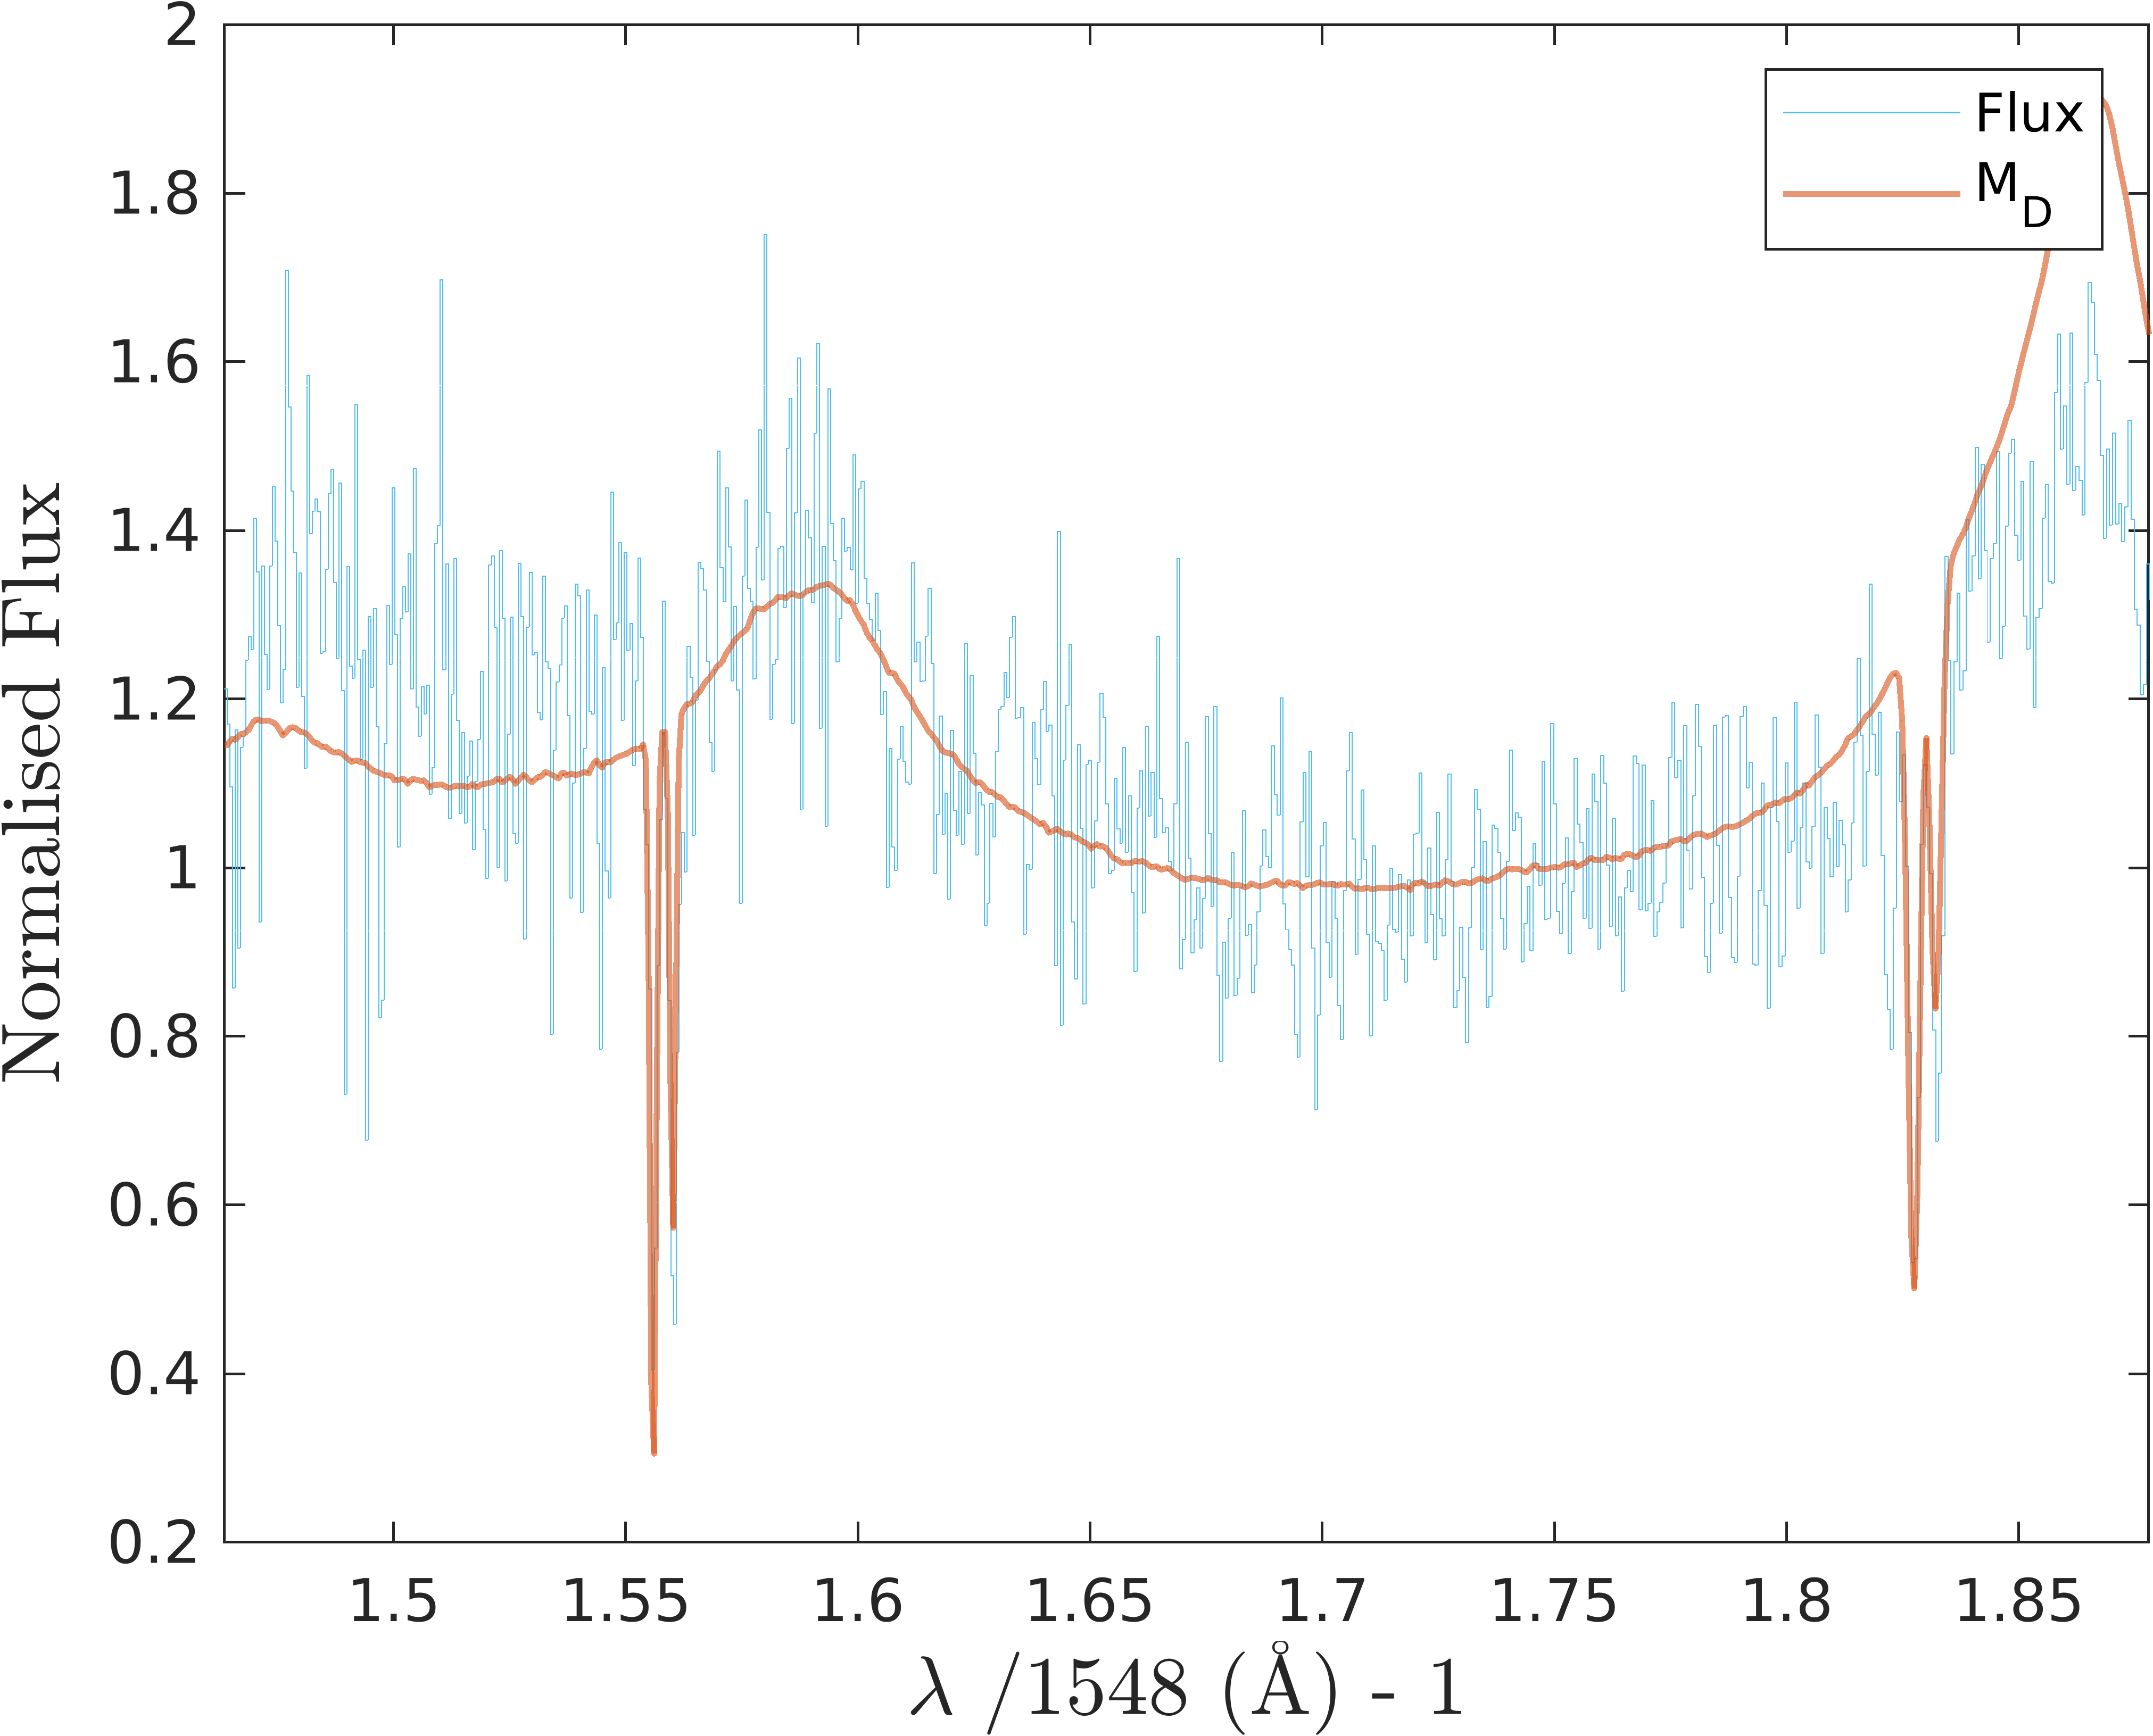
\includegraphics[width=0.75\linewidth]{figs/PM1GP0.png}
  \caption{Example of an absorber detected by the PM catalogue, but assigned a relatively low probability (34\%) by the GP catalogue, at $\zciv=1.827$.
The QSO-ID for this spectrum is 52367-0332-585, and the quasar redshift is $1.87$.
The posterior absorption probabilities are
 $P(CIV)=$[1.00, 1.00, 0.34, 0.15], with maximum a posterior absorber redshifts of
 $z_{CIV}$=[1.554, 1.826, 1.820, 1.692], and the rest equivalent widths are REW(GP)=[0.59, 0.88, 0.53, 0.26]\AA.
The PM catalogue reported absorbers at $z_{PM}$=[1.556,1.822,1.827] with
REW(PM)$=[0.88\pm 0.12$, $0.40\pm0.10$, $0.88\pm 0.08$]\AA.}
  \label{fig:PM1GP0}
\end{figure*}
 \begin{figure*}
  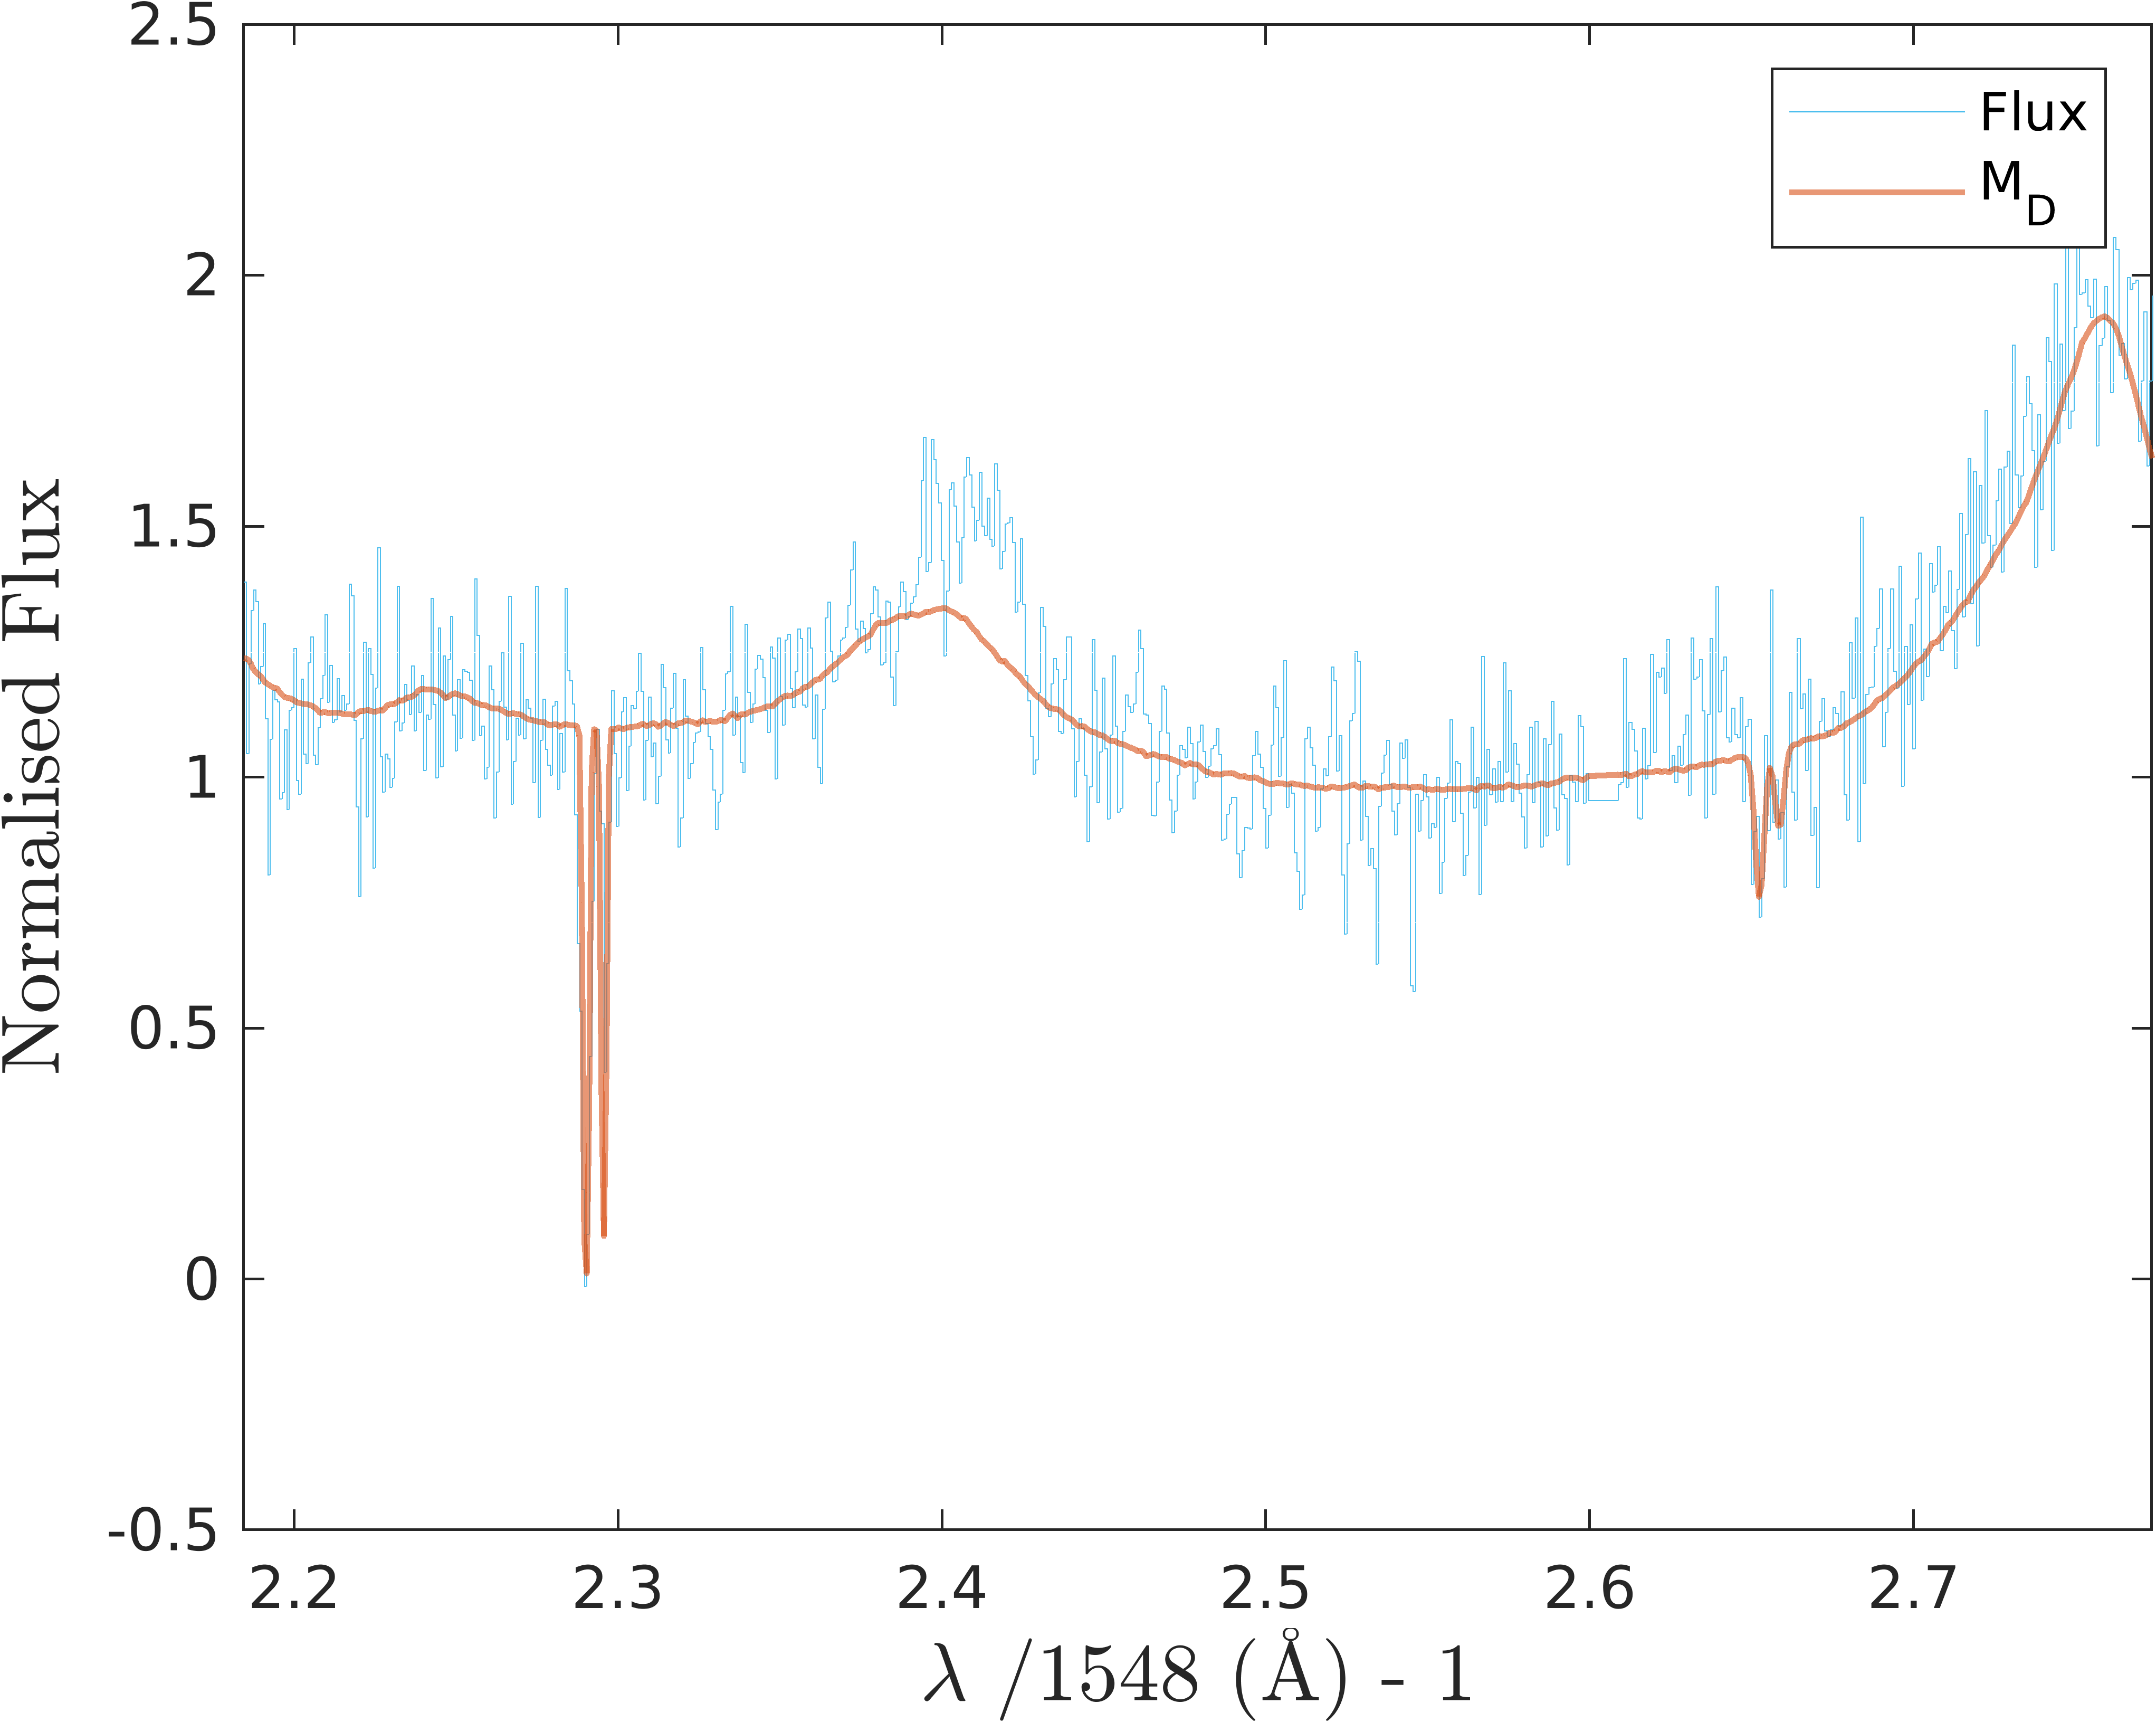
\includegraphics[width=0.75\linewidth]{figs/PM0GP1.png}
  \caption{Example spectrum with two absorbers found by GP with high probability missed by the PM catalogue.
  QSO-ID is 51994-0309-592 and $\zqso =  2.76$. Probabilities for the total 4 searches are:
 P(CIV)=[1.00, 0.98], the maximum a posteriori absorption redshift values are $z_{CIV}$=[2.288, 2.650],
 and the rest equivalent width from Voigt profile integration are REW(GP)=[0.90, 0.32]\AA.
The PM catalog reports no absorption for this spectrum.}
  \label{fig:PM0GP1}
\end{figure*}



% \subsection{Optimising the performance}

% \spb{Let's rephrase this as 'sensitivity of validation to hyperparameters'.
% Some of the below should be move to section 3. In particular, the discussion
% of different values of $k$ belongs in 3.2. The discussion of the prior ranges
% of N, sigma and z belong in the priors section. Here you just want to say which
% parameters you varied, and which ones did not affect the ROC.}
% \rmon{This is part of early versions of the draft. I fix it.}
% We try to maximize the purity and completeness by choosing the best parameters
% in our initializing
% script, \texttt{set\_parameters\_dr7.m}, which is a
% MATLAB script file in our GitHub
% repository\footnote{\href{https://github.com/rezamonadi/GaussianProcessCIV}{https://github.com/rezamonadi/GaussianProcessCIV}}
% where all of the controlling input parameters are initialised. These
% parameters appear in the learning and
% processing phases while running \texttt{learn\_qsos.m} and
% \texttt{process\_qsos\_dr7.m} in our GitHub repository.

% % We first describe the influential parameters which were examined in the learning phase.
% %     We learn a \civ-free model on the spectra of SDSS DR7 that
% %     have been investigated in PM-catalogue but appeared not to have a \civ\
% %     doublet.




\section{Results for SDSS DR12}
\label{sec:results}

We have used our model to find \civ\ absorbers in SDSS DR12. We searched for up to $7$ absorbers in $185,425$ \civ\ spectra of SDSS DR12.
For each spectrum, we provide probabilities for  \civ\ absorption. We also provide maximum a posteriori and 68\% credible
intervals for each of our model parameters $\{\nciv,~ \sciv,~ \zciv\}$.
Each of these products are a $185425\times7$ array. When the search terminated
finding fewer than $7$ absorbers, we report a NaN value for the columns associated with all further absorbers.

%     because
%     $P_n(\model_{N}) >P_n(\model_D), P_n(\model_{S})$,
The upper panel of Fig. \ref{fig:search12} illustrates the first \civ~search on "QSO-56265-6151-936" with $\zqso = 2.4811$. We found a $\civ$ absorber at $\zciv=2.135$. The null model had $P_n(\model_{N}) < 10^{-2}$, the single line model $P_n({\model_S})=0.04$, and the \civ\ doublet model $P_n({\model_D})=0.96$. We thus masked the \civ\ doublet model, and commenced the second
search, shown in the lower panel of Fig.~\ref{fig:search12}.
Our second search found an absorber at $\zciv=2.149$ with $P_n({\model_D})=0.98$,
$P_n({\model_S})=0.01$, and $P_n({\model_{N}})=0.01$.

    % We continued this searches ??? why not the 4th search?.
    % The lower panels of Fig.   \ref{fig:search1} and Fig. \ref{fig:search12} show the distribution of our sampled
    %   $\nciv$ and $\zciv$, given that  $\sciv$ is  10\kms the maximum a posteriori
    %    value for $\sciv$.

\begin{figure*}
  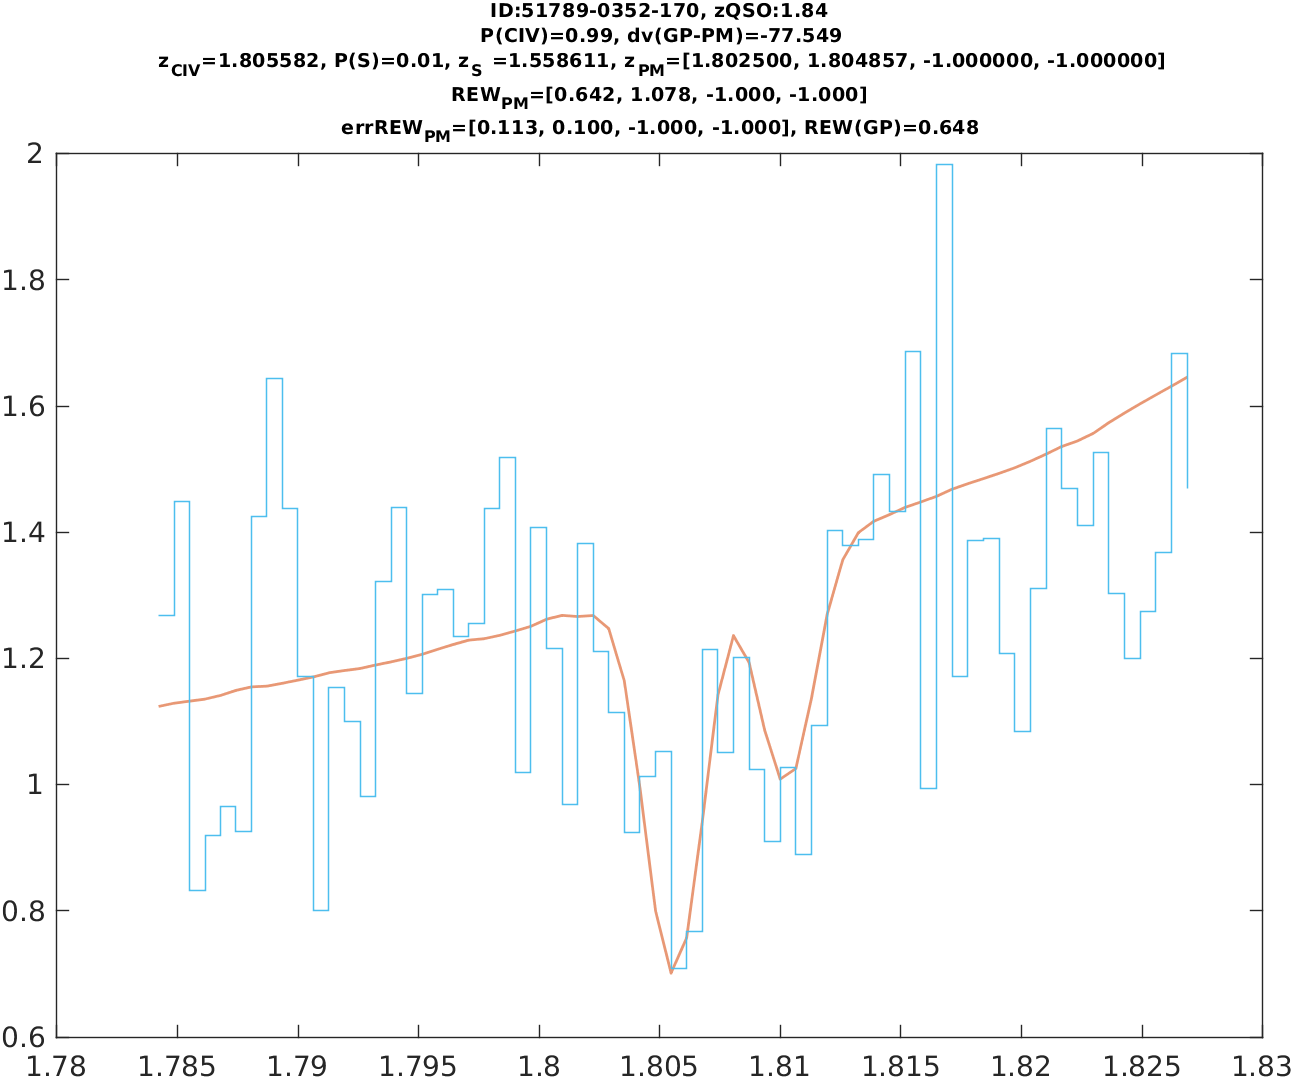
\includegraphics[width=0.9\linewidth]{figs/ind-32-c4-1.png}
  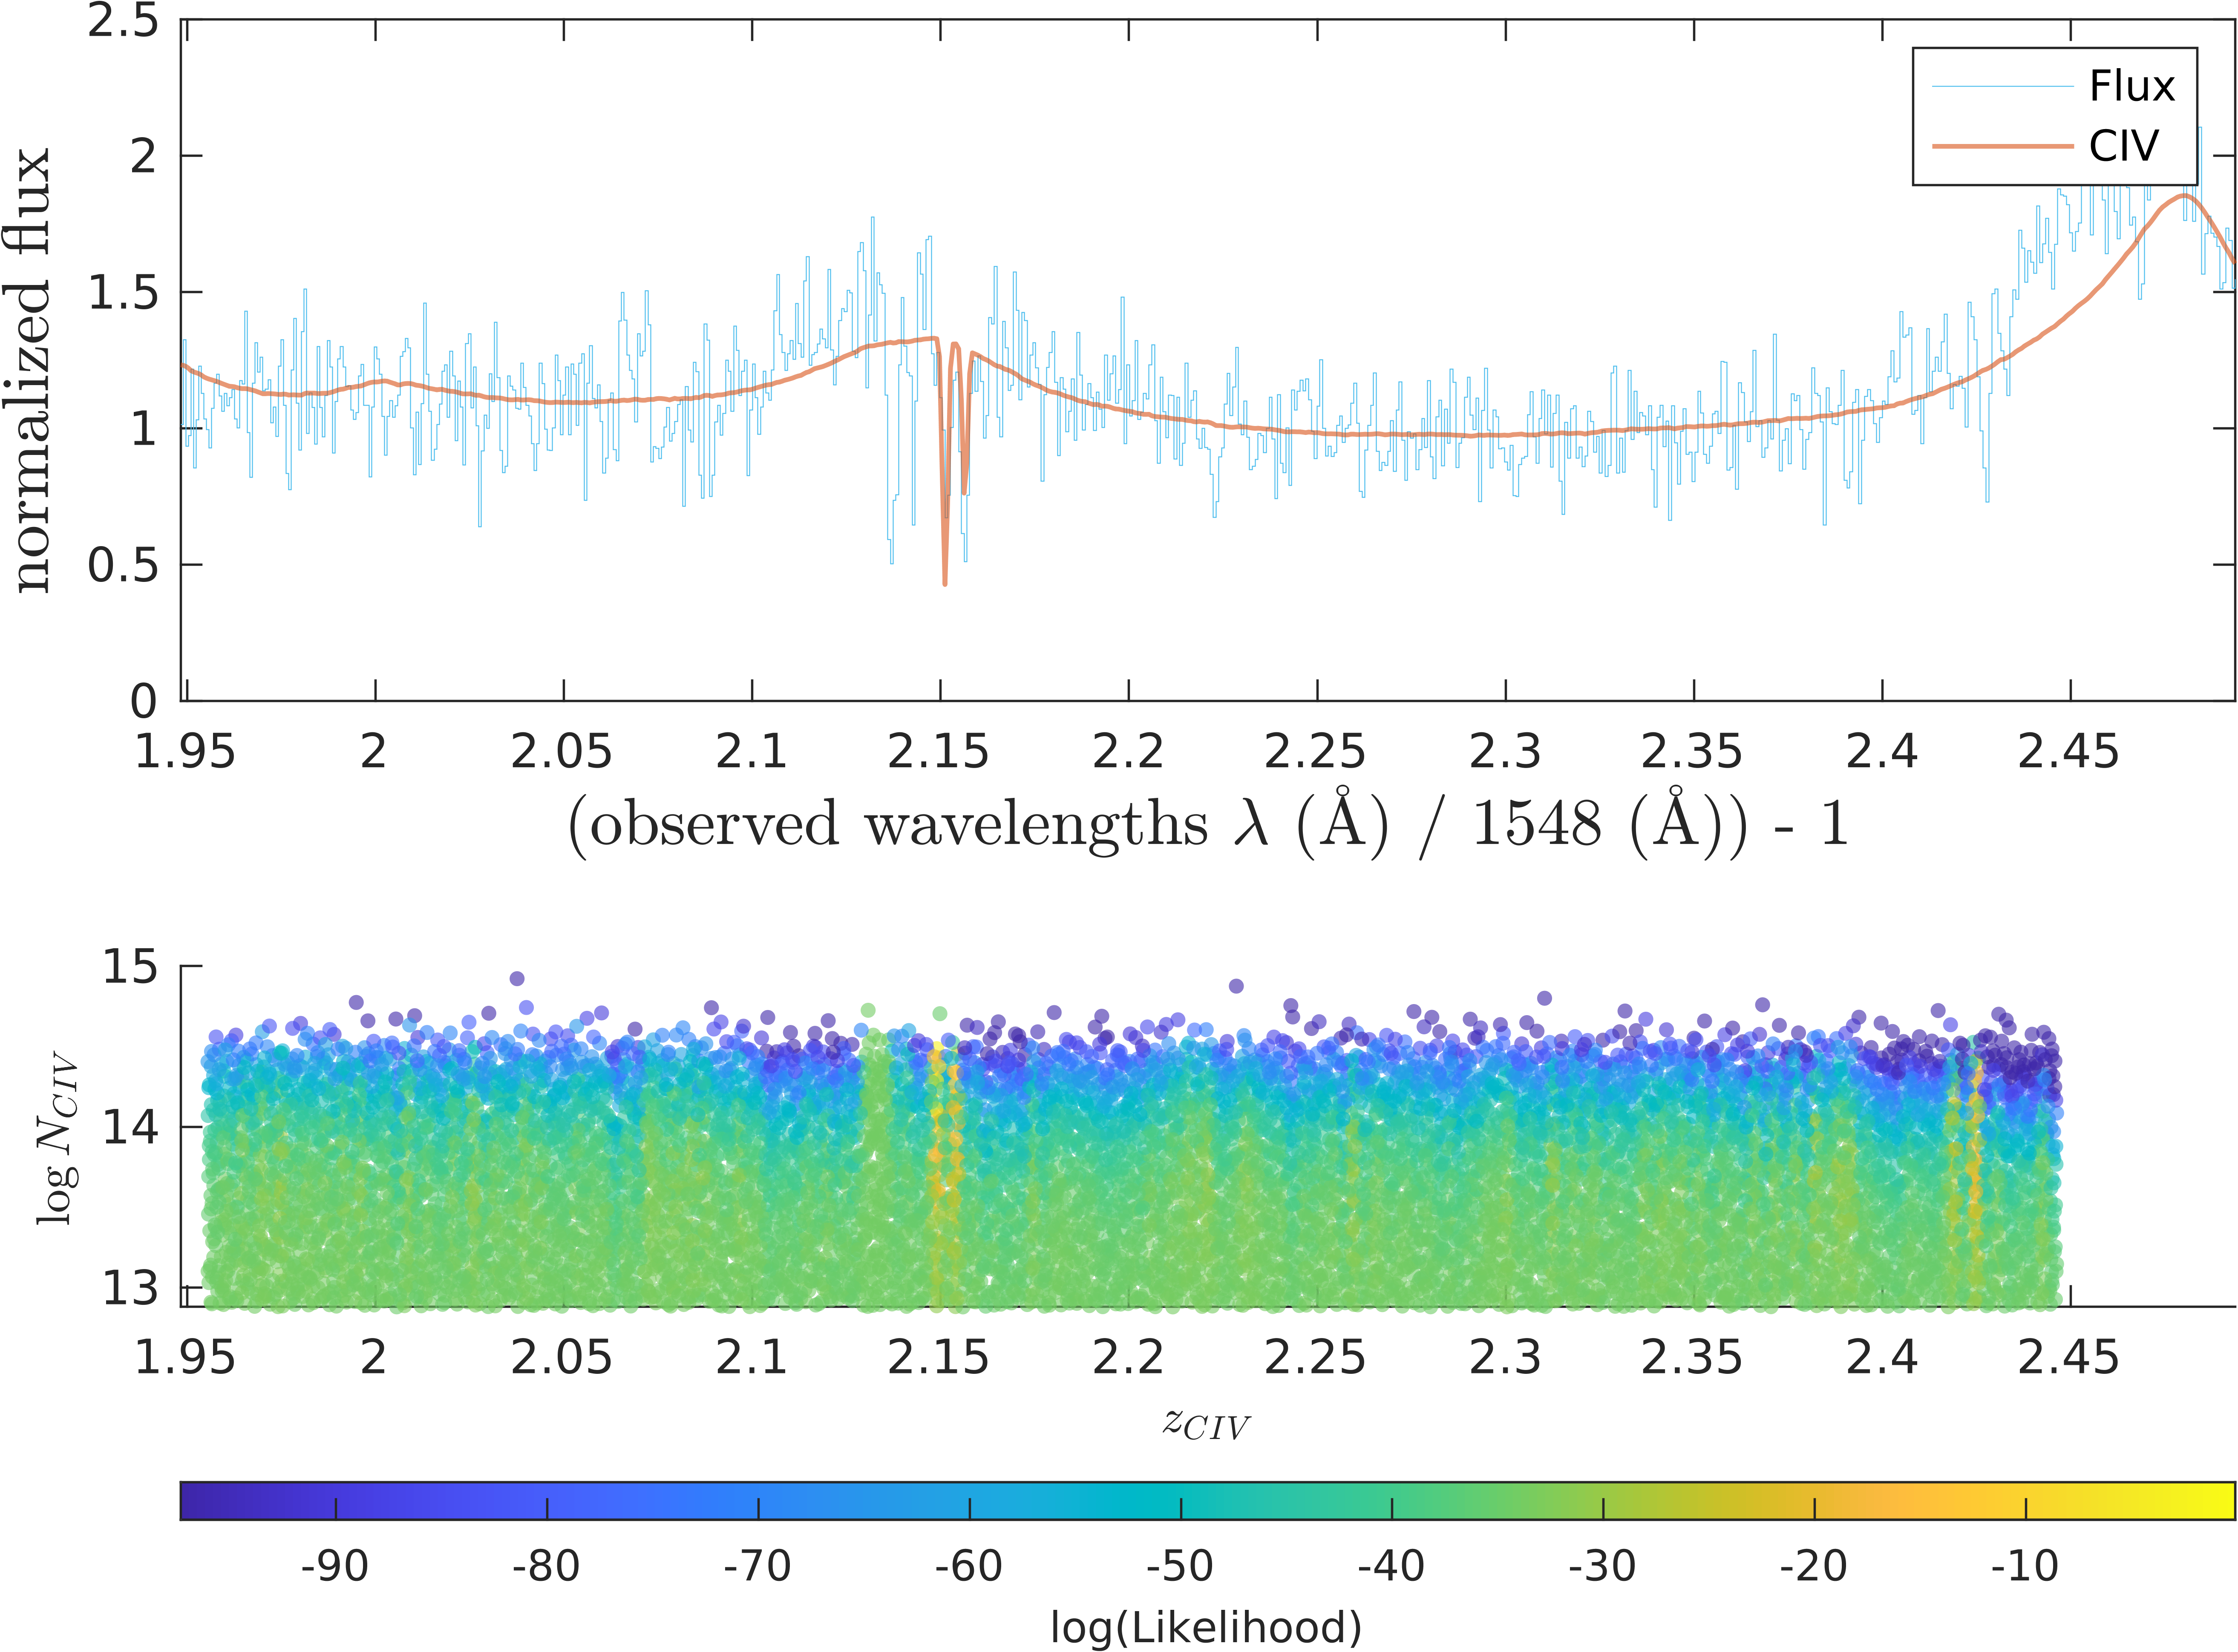
\includegraphics[width=0.9\linewidth]{figs/ind-32-c4-2.png}
  \caption{Upper panel: example spectrum showing the likelihood function for the first
   \civ~search. Lower panel: the same spectrum during a search for a
   second \civ~absorber, after masking the first absorption system.
    % P(\civ)= ?? map($\zciv$)= ??? REW(GP)= ?? QSO-ID=??? $\zqso$ =??
    }
  \label{fig:search12}
\end{figure*}

% Table of threshold 65\%, 85\%, and 95\%
Table \ref{tab:p_c4} summarises the reported posterior probabilities for our catalogue.
Around 66\% of spectra had no \civ\ absorbers detectable at more than 85\% certainty.
 Around 15\% of spectra had 1 absorber and $\sim 8\%$ had 2 absorbers.
  Note that this is much more than $0.15^2$ ($\sim 2.2\%$), demonstrating a
  strong correlation between absorbers. We find $5$ or more absorbers in only 3.1\% of spectra
  with $85\%$ probability. We detected a single line absorber in $\sim 10$\% of sightlines. The probability of finding two in a single sightline was $\sim 2\%$, so we did not detect a correlation between single line absorbers.

% \begin{table}
%   \caption{Table of probabilities (D): first column shows the number of \civ\ absorbers. The 2nd through 4th
%    columns   show the number of \civ~absorbers with probabilities > 65\%, 85\%, and 95\% respectively. } %The last row shows the total number of found absorbers with a certain probability threshold.
%   \label{tab:p_c4}
%     \begin{tabular}{|l|l|l|l|}
%     \hline
%     \civ &	$P_n(\model_D)>0.65$ &	$P_n(\model_D)>0.85$&	$P_n(\model_D)>0.95$\\ \hline
%     0 &	113002 (60.9\%)&	123897 (66.8\%)&	131586 (71\%)\\
%     1	& 30801	(16.6\%)&27441	(14.8\%)&24825 (13.3\%)\\
%     2	& 17307 (9.3\%)&	14255 (7.7\%)	&12539 (6.7\%)\\
%     3	&9869	(5.3\%)&8341 (4.5\%)&	7136 (3.8\%)\\
%     4&	6274 (3.4\%)&	5207 (2.8\%)&	4427 (2.4\%)\\
%     5	&4473 (2.4\%)	&3553	(1.9\%)&2853 (1.5\%)\\
%     6&	2626	(1.4\%) &1948 (1.05\%)&	1469 (0.8\%)\\
%     7& 1073 (0.57\%)& 783 (0.42\%) & 590 (0.31\%)\\
%     % Total & 165750 & 136736 &	116228
%       \end{tabular}
% \end{table}

\begin{table}
  \caption{Table of probabilities (D): first column shows the number of \civ\ absorbers. The 2nd through 4th
   columns   show the number of \civ~absorbers with probabilities > 65\%, 85\%, and 95\% respectively. } %The last row shows the total number of found absorbers with a certain probability threshold.
  \label{tab:p_c4}
    \begin{tabular}{|l|l|l|l|}
    \hline
    \civ &	$P_n(\model_D)>0.65$ &	$P_n(\model_D)>0.85$&	$P_n(\model_D)>0.95$\\ \hline
    0 &	113142 (61.0\%)&	123994 (66.8\%)&	131767 (71.0\%)\\
    1	& 31163	(16.8\%)& 27733	(14.9\%) & 24981 (13.5\%)\\
    2	& 17526 (9.4\%)&	14533 (7.8\%)	& 12777 (6.9\%)\\
    3	& 10020	(5.4\%)& 8424 (4.5\%)&	7218 (3.9\%)\\
    4&	6112 (3.3\%)&	4960 (2.6\%)&	4176 (2.3\%)\\
    5	& 4155 (2.2\%)	& 3342	(1.8\%)& 2656 (1.4\%)\\
    6&	2426	(1.3\%) & 1771 (0.9\%)&	1348 (0.7\%)\\
    7& 881 (0.5\%)& 668 (0.4\%) & 502 (0.3\%)\\
    % Total & 165750 & 136736 &	116228
      \end{tabular}
\end{table}

%Figures~\ref{fig:DR12Z}, \ref{fig:DR12N} and \ref{fig:DR12Sigma} show histograms of the maximum a posteriori values for each model parameter
% in the searched DR12 spectra.
Fig. \ref{fig:DR12Z} shows the distribution of (maximum a posteriori) absorber redshifts.
There is a peak around $z\sim 2$, mirroring the distribution of quasar 
redshifts. Overall, we have detected an order of magnitude more absorbers 
than the PM catalogue, reflecting the larger size of our sightline sample.
There are $33$ absorbers in DR12 with  $P_n{\model_D}>0.85$
and a redshift higher than $4.68$, the maximum reported
$\zciv$ in the PM catalogue.
% \spb{Can you write a comparison of the high redshift results
%  to DR7? What is the highest redshift absorber in our catalogue compared
%  to the DR7 catalogue? How many absorbers do we have at a redshift higher than the one in DR7?}

\begin{figure}
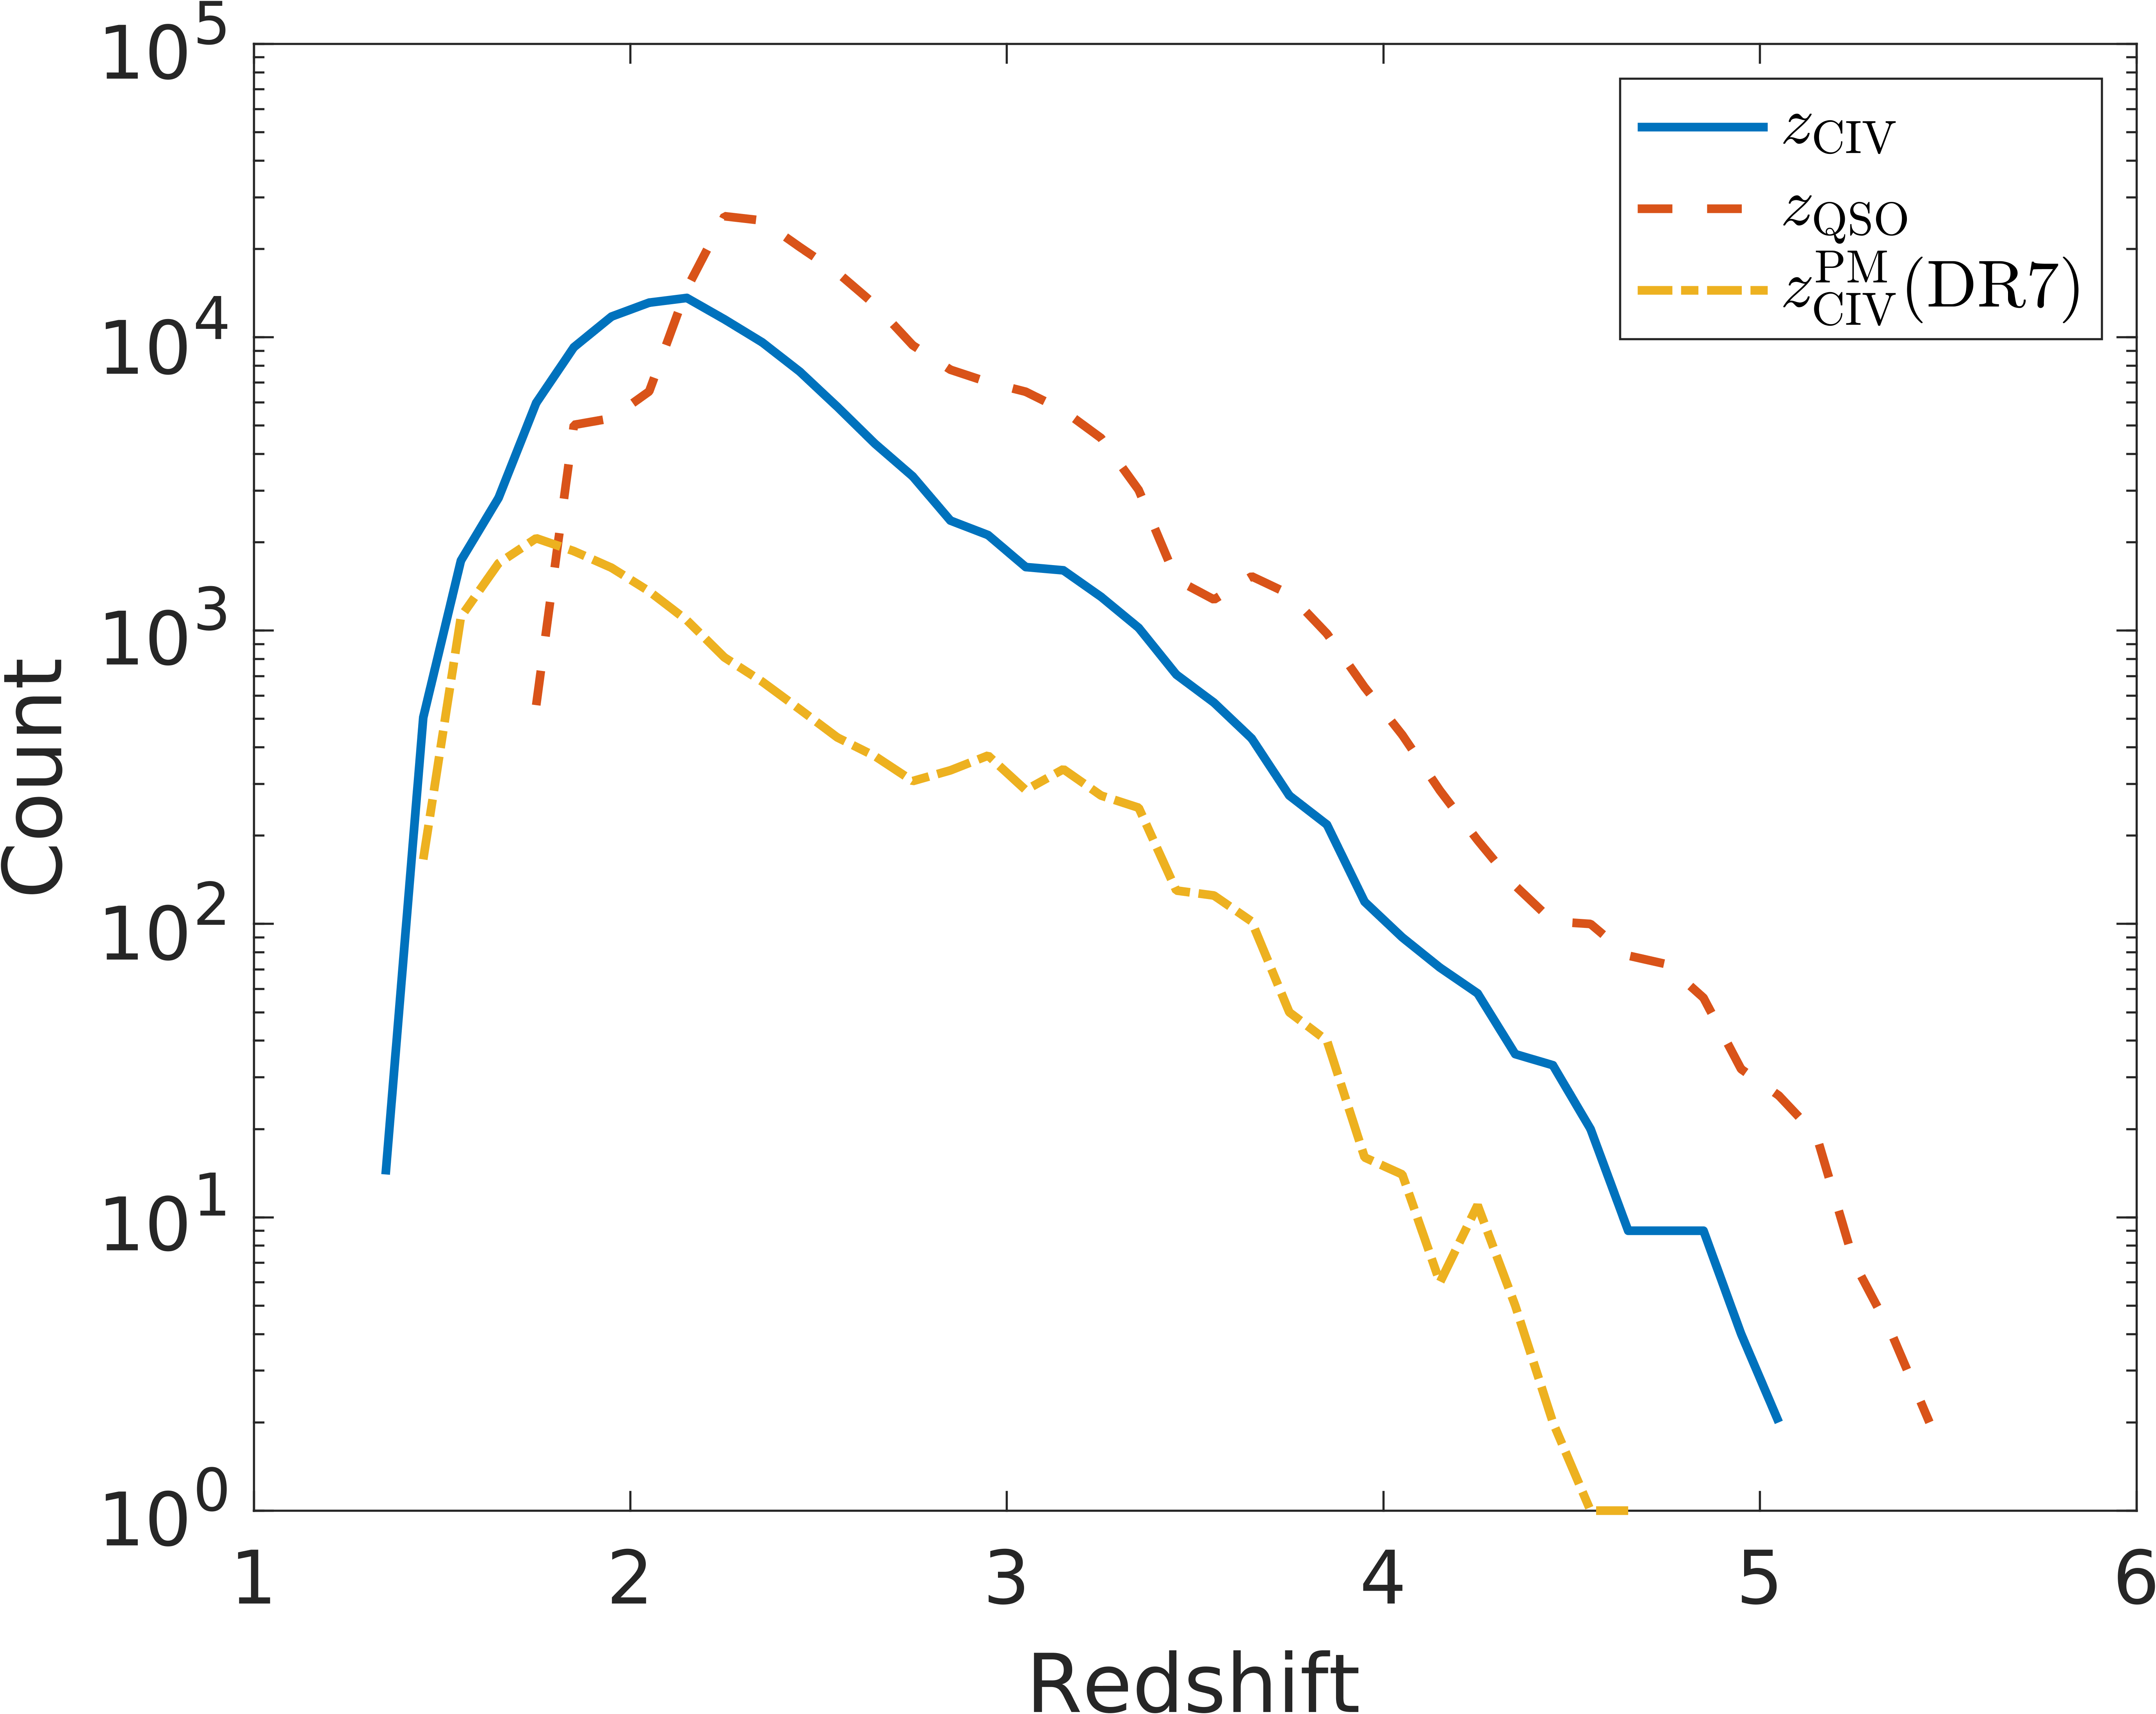
\includegraphics[width=\linewidth]{figs/histDR12_ZP95_curve_Z_c13_ZQSO.png}
\caption{Blue curve: Distribution of the maximum a posteriori values for all absorber redshifts
with $P_n{\model_D}>0.95$ in SDSS DR12 spectra. Red curve: Distribution of quasar redshift value in
our testing set in SDSS DR12. Yellow curve; Distribution of $\zciv$ in our catalogue. }
\label{fig:DR12Z}
\end{figure}


In Fig. \ref{fig:DR12Sigma} we show the distribution
of maximum a posteriori values of absorber
Doppler sigma parameters for the searched absorbers in the tested spectra. While
the prior distribution for Doppler sigma parameters was flat between 35 \kms to
115 \kms, we see that our absorbers follow a bimodal distribution in
$\sciv$ values. The second peak of larger $\sciv$ values is connected with
larger column densities. We examined the spectra of detected
absorbers with $\nciv > 16$ and $\sciv > 110$ \kms. Most of these spectra are noisy and
in some cases the line is heavily blended.
% \footnote{ \url{http://data.sdss3.org/sas/dr12/boss/qso/DR12Q/DR12Q_BAL.fits} }.
The mean S/N around detected \civ\ absorbers with probability larger than
85\% is $6.8$, compared to a mean S/N of $2.5$ for spectra
that contain absorbers with $\sciv>80$ \kms and $\nciv>15$. %with a probability larger than 85\%,

\begin{figure}
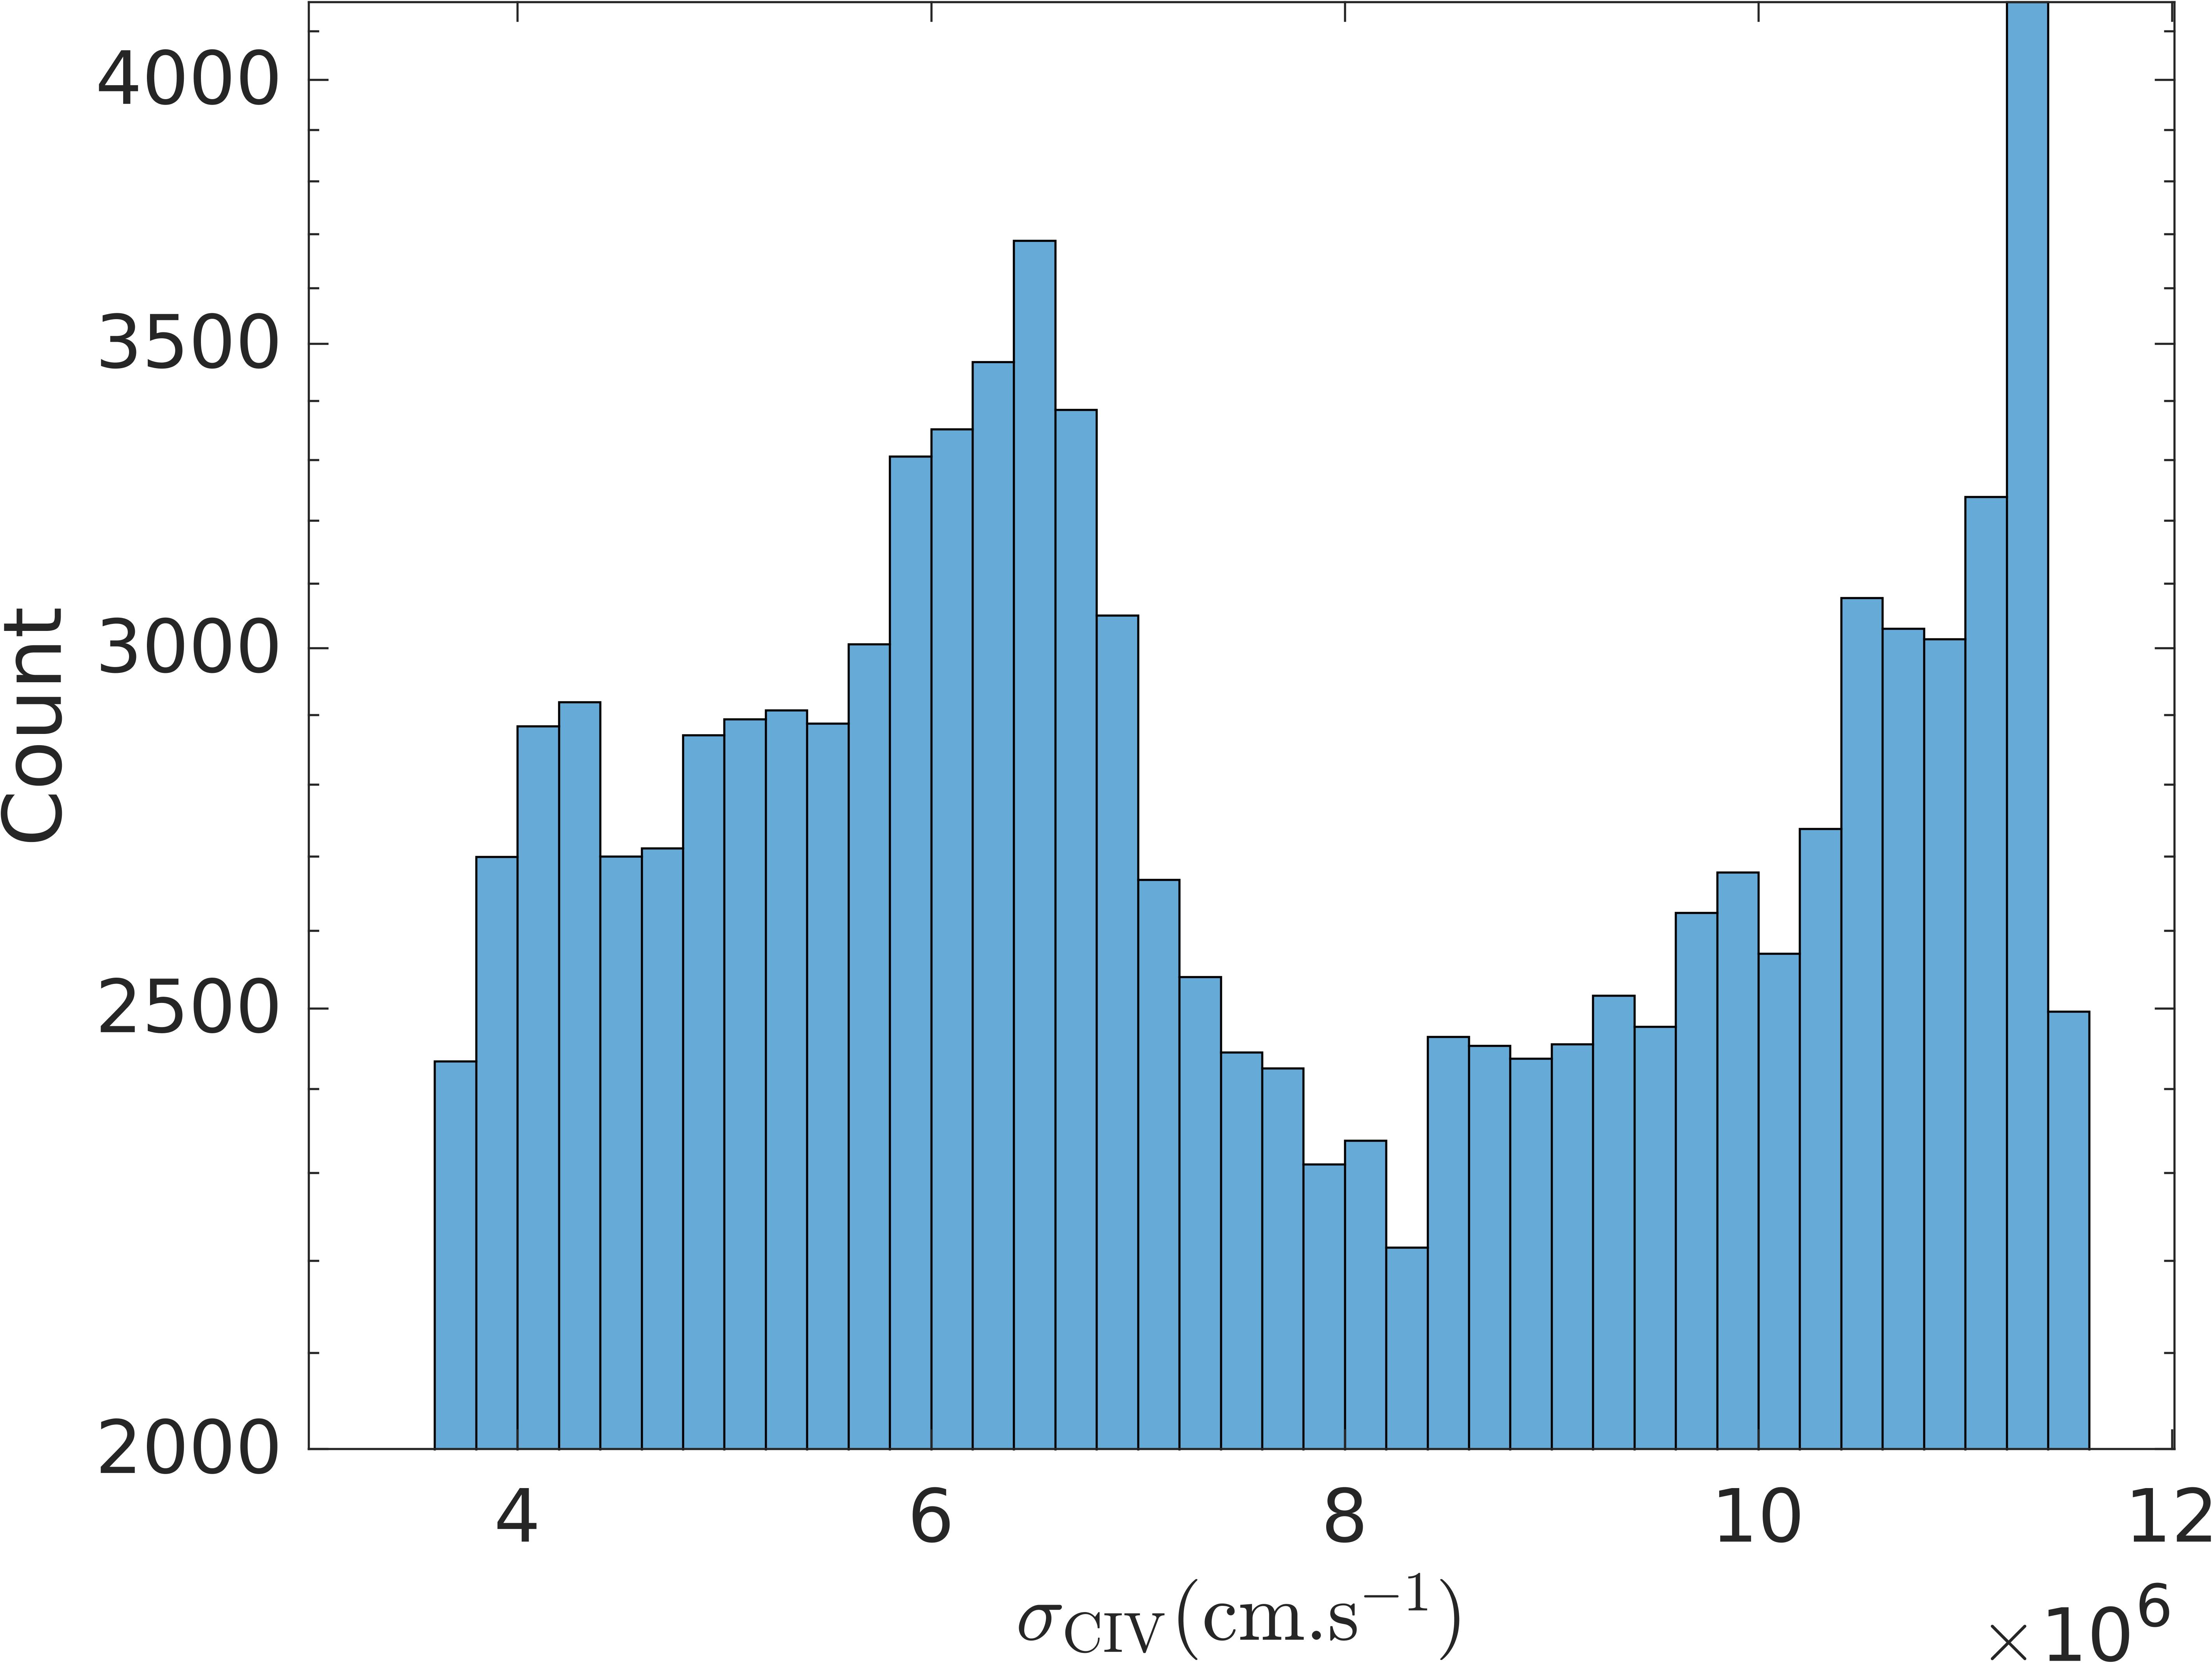
\includegraphics[width=\linewidth]{figs/histDR12_SigmaP95.png}
\caption{Distribution of the maximum a posterior values for all
 searched Doppler sigma parameters
in SDSS DR12 spectra with $P_n(\model_D)>0.95$. }
\label{fig:DR12Sigma}
\end{figure}

    % P_n(Model_GP)
    Figure~\ref{fig:distp1} shows the distribution of probabilities for observing
    $1$ through $4$ \civ\ absorbers in the spectra in SDSS DR12.
    For each search we see a peak in the posterior probability distribution around 30\%, stronger at earlier searches.
    \begin{figure}
      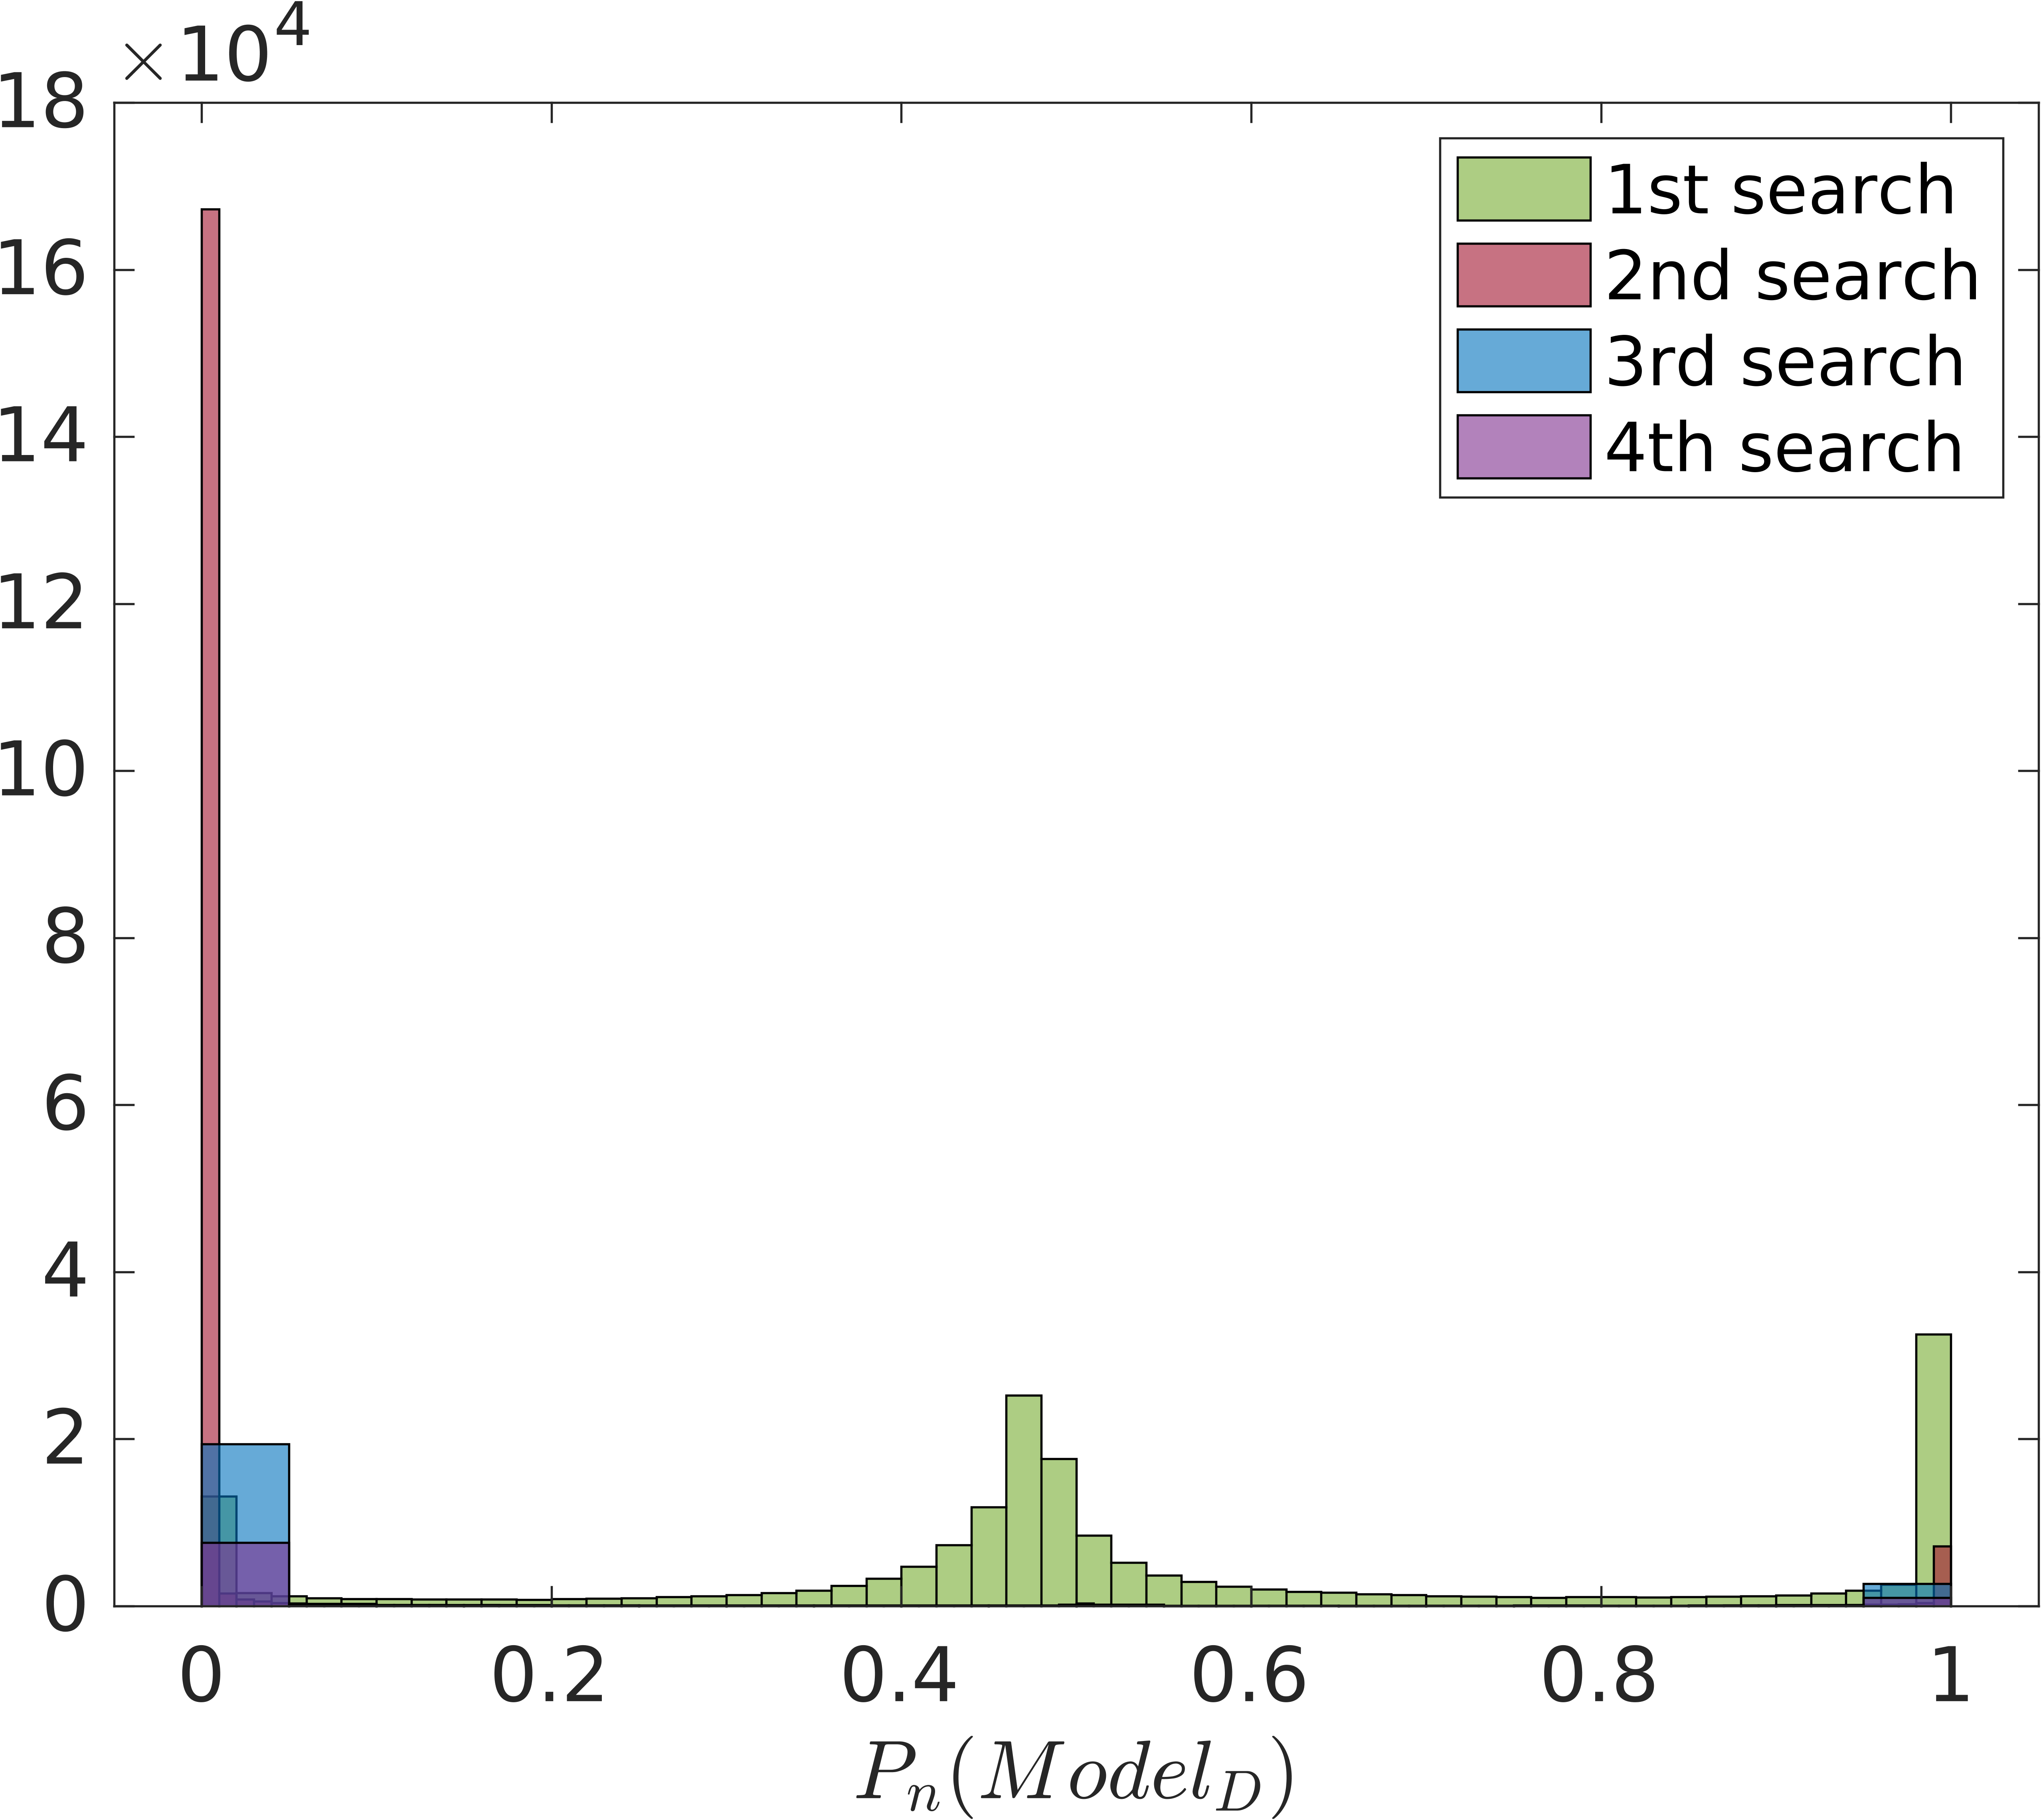
\includegraphics[width=\linewidth]{figs/pDistAll.png}
      \caption{Distribution of $P_n(\model_D)$ for all of the searches from 1st to 4th one.
      We did not show other searches as they are less important and we find very few absorbers after
      the 4th search (see Table \ref{tab:p_c4}).}
      \label{fig:distp1}
    \end{figure}
    We looked at the distribution of $P_n(\model_S)$ for the 1st search as well as
    $P_n(\model_{N})$ and it was clear that many of these ambiguous \civ~absorbers
    also have $P_n(\model_S) \sim 0.3$. In addition, these
    absorbers are in generally lower S/N spectra. Thus these potential absorbers are those where the spectra are weakly constraining and the absorber probability is dominated by the priors.
%    \rmon{Note that when the S/N is low, there is  relatively
%    lower chance that the data have been generated by any of the models (i.e. low likelihood). As a
%    result the model posteriors are mostly affected by the prior probability.}

    %EW
    In Fig. \ref{fig:DR12-DR7-REW} we show REW(1548\AA) from our 
    SDSS DR12 catalogue. The REW is uncorrelated with posterior 
    probability of absorption strength. We also show the DR7 PM 
    catalogue REW distribution for comparison. Our catalogue 
    is more sensitive to weaker absorbers and the larger statistical sample allows us to probe higher REW, with \rmon{110} 
    absorbers at larger REW than the highest value seen in the PM catalogue.

    \begin{figure}
      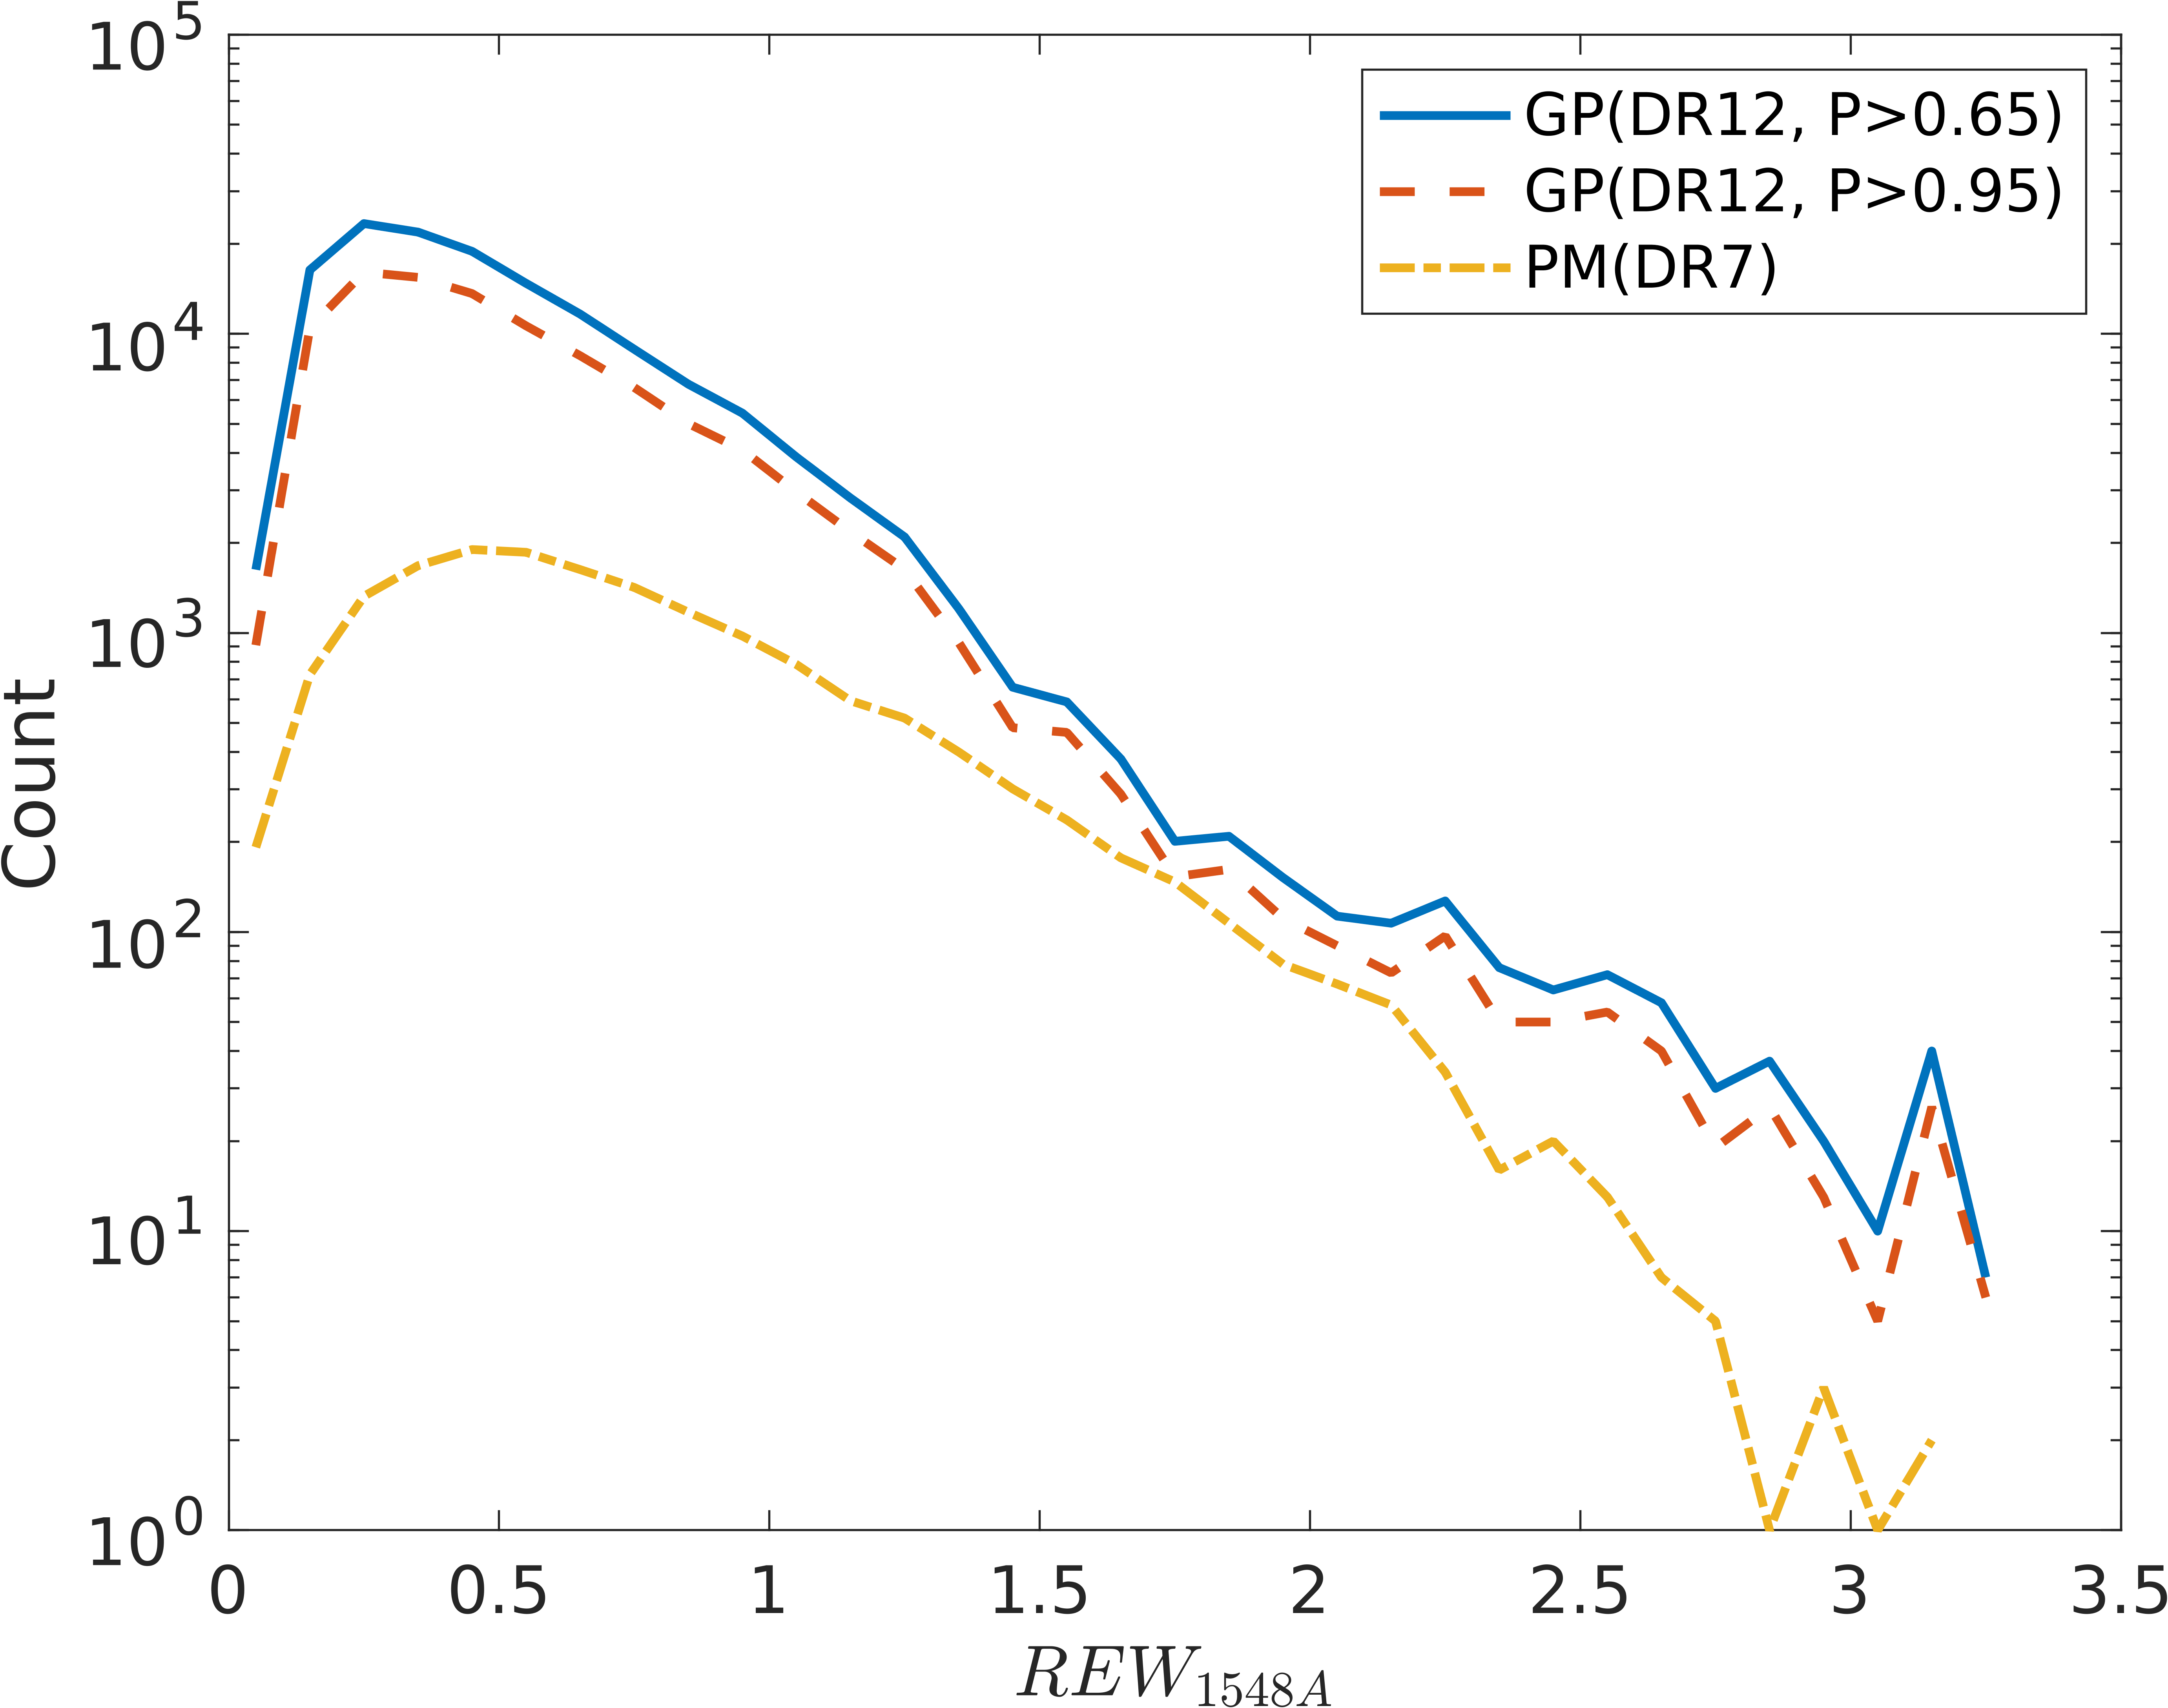
\includegraphics[width=\linewidth]{figs/REW_1548_GP_PM_SW_2.png}
      \caption{Distribution of the maximum a posteriori values
      of REW(1548\AA) for all searched absorbers
      in SDSS DR12 spectra with  $P_n{\model_D}>0.65$, 
       and $P_n{\model_D}>0.95$.
      We also show for comparison REW values from the PM catalogue.}
      \label{fig:DR12-DR7-REW}
      \end{figure}

    Fig. \ref{fig:DR} shows the distribution of the doublet ratio, REW(1548\AA)/REW(1550\AA), obtainedby integrating the Voigt profile at the maximum a posteriori values of
    $\{\zciv, \nciv, \sciv\}$. Most of our Voigt profiles are close to the
 linear curve of growth value of $2$, but there is a tail of lower doublet ratios when one of the absorbers are saturated.

  \begin{figure}

     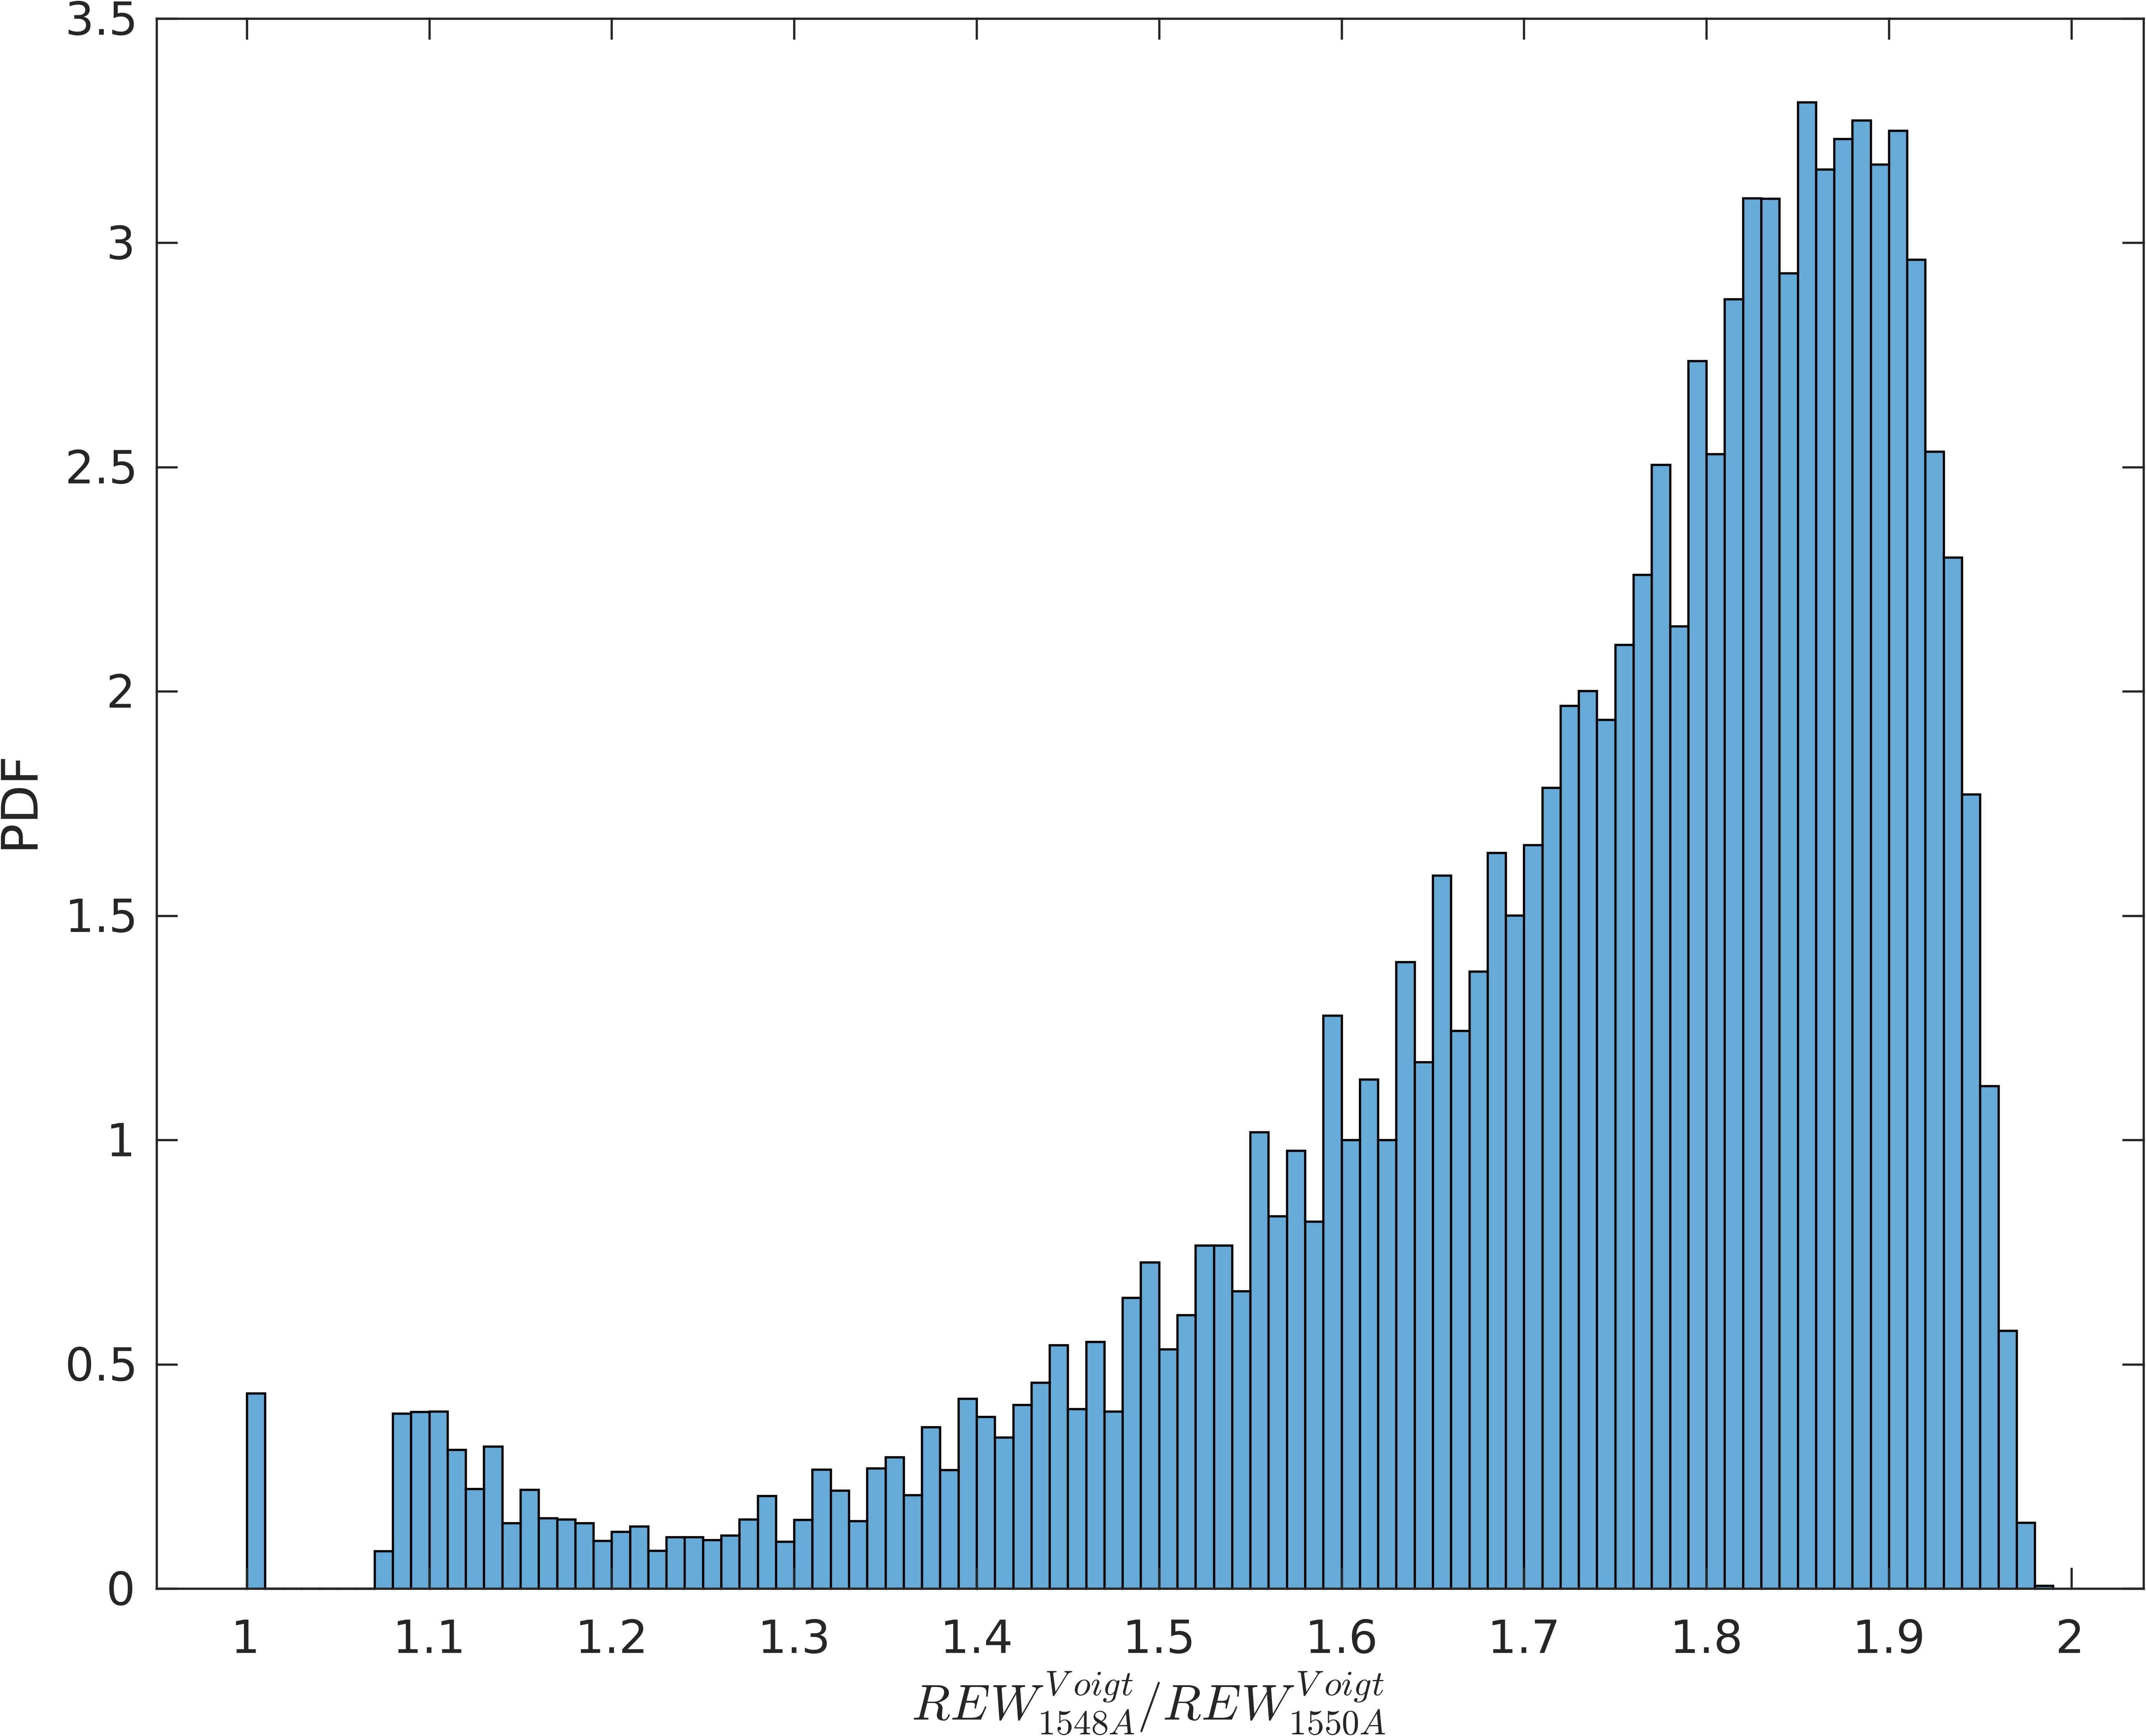
\includegraphics[width=\linewidth]{figs/DR_1550_1548_voigt.png}
     \caption{Distribution of the doublet ratio, REW(1548\AA)/REW(1550\AA). The
     REW values are calculated based on our Voigt profile integration. }
     \label{fig:DR}
  \end{figure}



    % We are aware that
    % the difference between these two REW values should not be much larger than the estimated error
    % coming from the noise in the observed flux. To check this, we plotted the ratio of difference between
    % err(REW) and $\Delta(REW)$ and the error from integrating flux in Fig. \ref{fig:errDiffREW}.
    % We see that these two measures estimate REW  consistently as
    % we have  a Gaussian distribution for this ratio.

\section{Conclusions}
\label{sec:summary}
We trained a quasar continuum model to detect \civ~absorbers using a Gaussian process. Training was done on a sample of DR7 spectra which were labelled as \civ~free in the Precious Metals catalogue of \cite{C13}. We used Bayesian model selection to compare our continuum model to one containing a \civ~doublet, and built a single line absorber model to avoid confusion from interloping metal lines.
The prior distribution was taken from our training catalog and flat parameter priors were used for the \civ~redshift, $\zciv$ and Doppler width $\sciv$. We searched for up to 7 absorbers in each tested spectrum and provide a comprehensive catalogue containing detection probability, as well as a maximum a posteriori value and credible interval for $\zqso$, $\nciv$ and $\sciv$. We validated our pipeline by applying it to a hold-out sample of $1301$ spectra from the PM catalogue. Our pipeline produced similar results to the PM catalogue and has good purity and completeness. Generally the two catalogues produced similar \civ~redshifts and rest equivalent widths.

Thus validated, we applied our model to SDSS DR12, and produced the largest \civ\ absorption catalogue yet seen. Among total 185425 selected quasar spectra in SDSS DR12, we found 113775
\civ\ doublets with at least 95\% probability. One can select absorbers in our catalogue with any level
of confidence thanks to our reported posterior probabilities for 
each absorber. We provide a posterior distribution for 
$\zqso$, $\nciv$ and $\sciv$ to aid in follow-up analyses. 
We detected \civ~absorption up to $z \sim 5$, including $33$
 systems at higher redshift than seen in DR7. We also detect 110 absorbers 
 with a rest equivalent width larger than the maximum in DR7 catalogue.

Our catalogue can be used to find targets for high resolution follow-up, to study complex \civ~systems. Alternatively it could be cross-matched with galaxy catalogues to find the properties of the galaxy CGM near to our \civ\ absorbers. Finally, statistical properties of our catalogue can be computed and compared to the outputs of cosmological simulations to test and improve models for galactic feedback.
%for informing their models about any initial conditions
%that might be involved by the statistics of \civ\ absorbers.
% Also they can compare their simulations \civ\ output with this catalogue.
% Discussion
% Discussion about sensitivity, completeness\\
% Discussion about the importance of a naked \civ catalogue or
% incorporation information about other metal lines and DLA catalogue.\\
% For the level of Signal-to-Noise in the SDSS spectra, we cannot really rely on the
% measured $\nciv$ and $\sciv$; the main focus should be on the $\zciv$. \\
In future work we will build a similar catalogue for SDSS DR16 and the Dark Energy Spectroscopic Instrument quasar survey. We will compare with a similar Damped Lyman-$\alpha$ catalogue and thus investigate the relationship between the highly ionized carbon and neutral hydrogen in the circumgalactic medium.

\section*{Acknowledgement}

R.M. was supported by Higher Education Emergency Relief Funds and S.B. was supported by NASA ATP 80NSSC22K1897.
We used the HPCC cluster at UC Riverside and AWS credits provided under an amazon machine learning research award. M.H. was supported by NASA FINESST grant 80NSSC21K1840.

\section*{Data availability}

All of our codes are available
publicly at  \href{https://github.com/rezamonadi/GaussianProcessCIV}
{GaussianProcessesCIV GitHub repository}
\footnote{https://github.com/rezamonadi/GaussianProcessCIV} and our final catalogue
can be found at \href{????}{????}\footnote{https://github.com/rezamonadi/???}.


% This is the section that people usually read.
% Talk about the entire workflow here, too.
% Main results with bullet points.
% Having A, doing B, we got C, as we expected in the intro.

% \section{Check-list}
% \begin{itemize}
%   \item Consistent active present tense
%   \item Every paragraph must have a separate point to convey
%   \item Most paragraphs: a mini intro, narrative and  conclusion
%   \item Remove filler words
%   \item replace a very large fraction" or "much of the data" say "90% of the data"
%   \item no forward or backward referencing:
%   \begin{itemize}
%     \item as we mentioned in section:
%     we will discuss in sec--> paper is not well organized
%   \end{itemize}
%   \item A very short writing guide:
%   \begin{itemize}
%     \item Impose structure.
%     \item Define the purpose of each paragraph (use comments).
%     \item State the "why" before the "how."
%     \item Use the figure captions to convey key science points.
%     \item Quantify
%     \item Clarify.
%     \item Proof-read out loud
%   \end{itemize}
%   \item  Keep your reader in mind.
%   \item Focus your paper on a central contribution, which you
%   communicate in the title.
%   \item minimize the number of loose threads that the reader has to keep in
%   mind at any one
%   time.
%   \item Define technical terms clearly
%   \item Stick to the context-content-conclusion (C-C-C) scheme
%   \item Reader cares about the result and logic, not the chronological path
%   \item avoid zig-zag
%   \item Use same wording for the same concept


% \end{itemize}



% Don't change these lines
\bsp	% typesetting comment
\label{lastpage}
\input{bib.tex}

\appendix
\section{Supporting information }
Fig. \ref{fig:DR12N} shows the distribution of maximum a posteriori column density values
for the searched absorbers in SDSS DR12. This is logarithmic scale for the abundance of
    absorbing systems. The trend for weaker systems is mostly reflecting the lower sensitivity
    of our method for weaker systems meaning that we rarely can put a high probability for
    a weak system in the level of S/N for our testing spectra.
     The power law trend for stronger systems than $\nciv\sim$15.5 turns into a
      flat distribution.


      We did a rest equivalent width consistency check similar to what we did in the validation phase.
    Fig. \ref{fig:errDiffREW} shows the difference between REW when we calculate
    it with boxcar summation using the observed fluxes:
    \begin{equation}
      REW\_Flux = \int_{1548-\delta\lambda}^{1548+\delta\lambda} \frac{F(\lambda)-C(\lambda)}{F(\lambda)}d\lambda
      \label{eq:rew_flux}
    \end{equation}
    and when we simply integrate the Voigt profile using Eq. \ref{eq:rewgp}.

\begin{figure}
  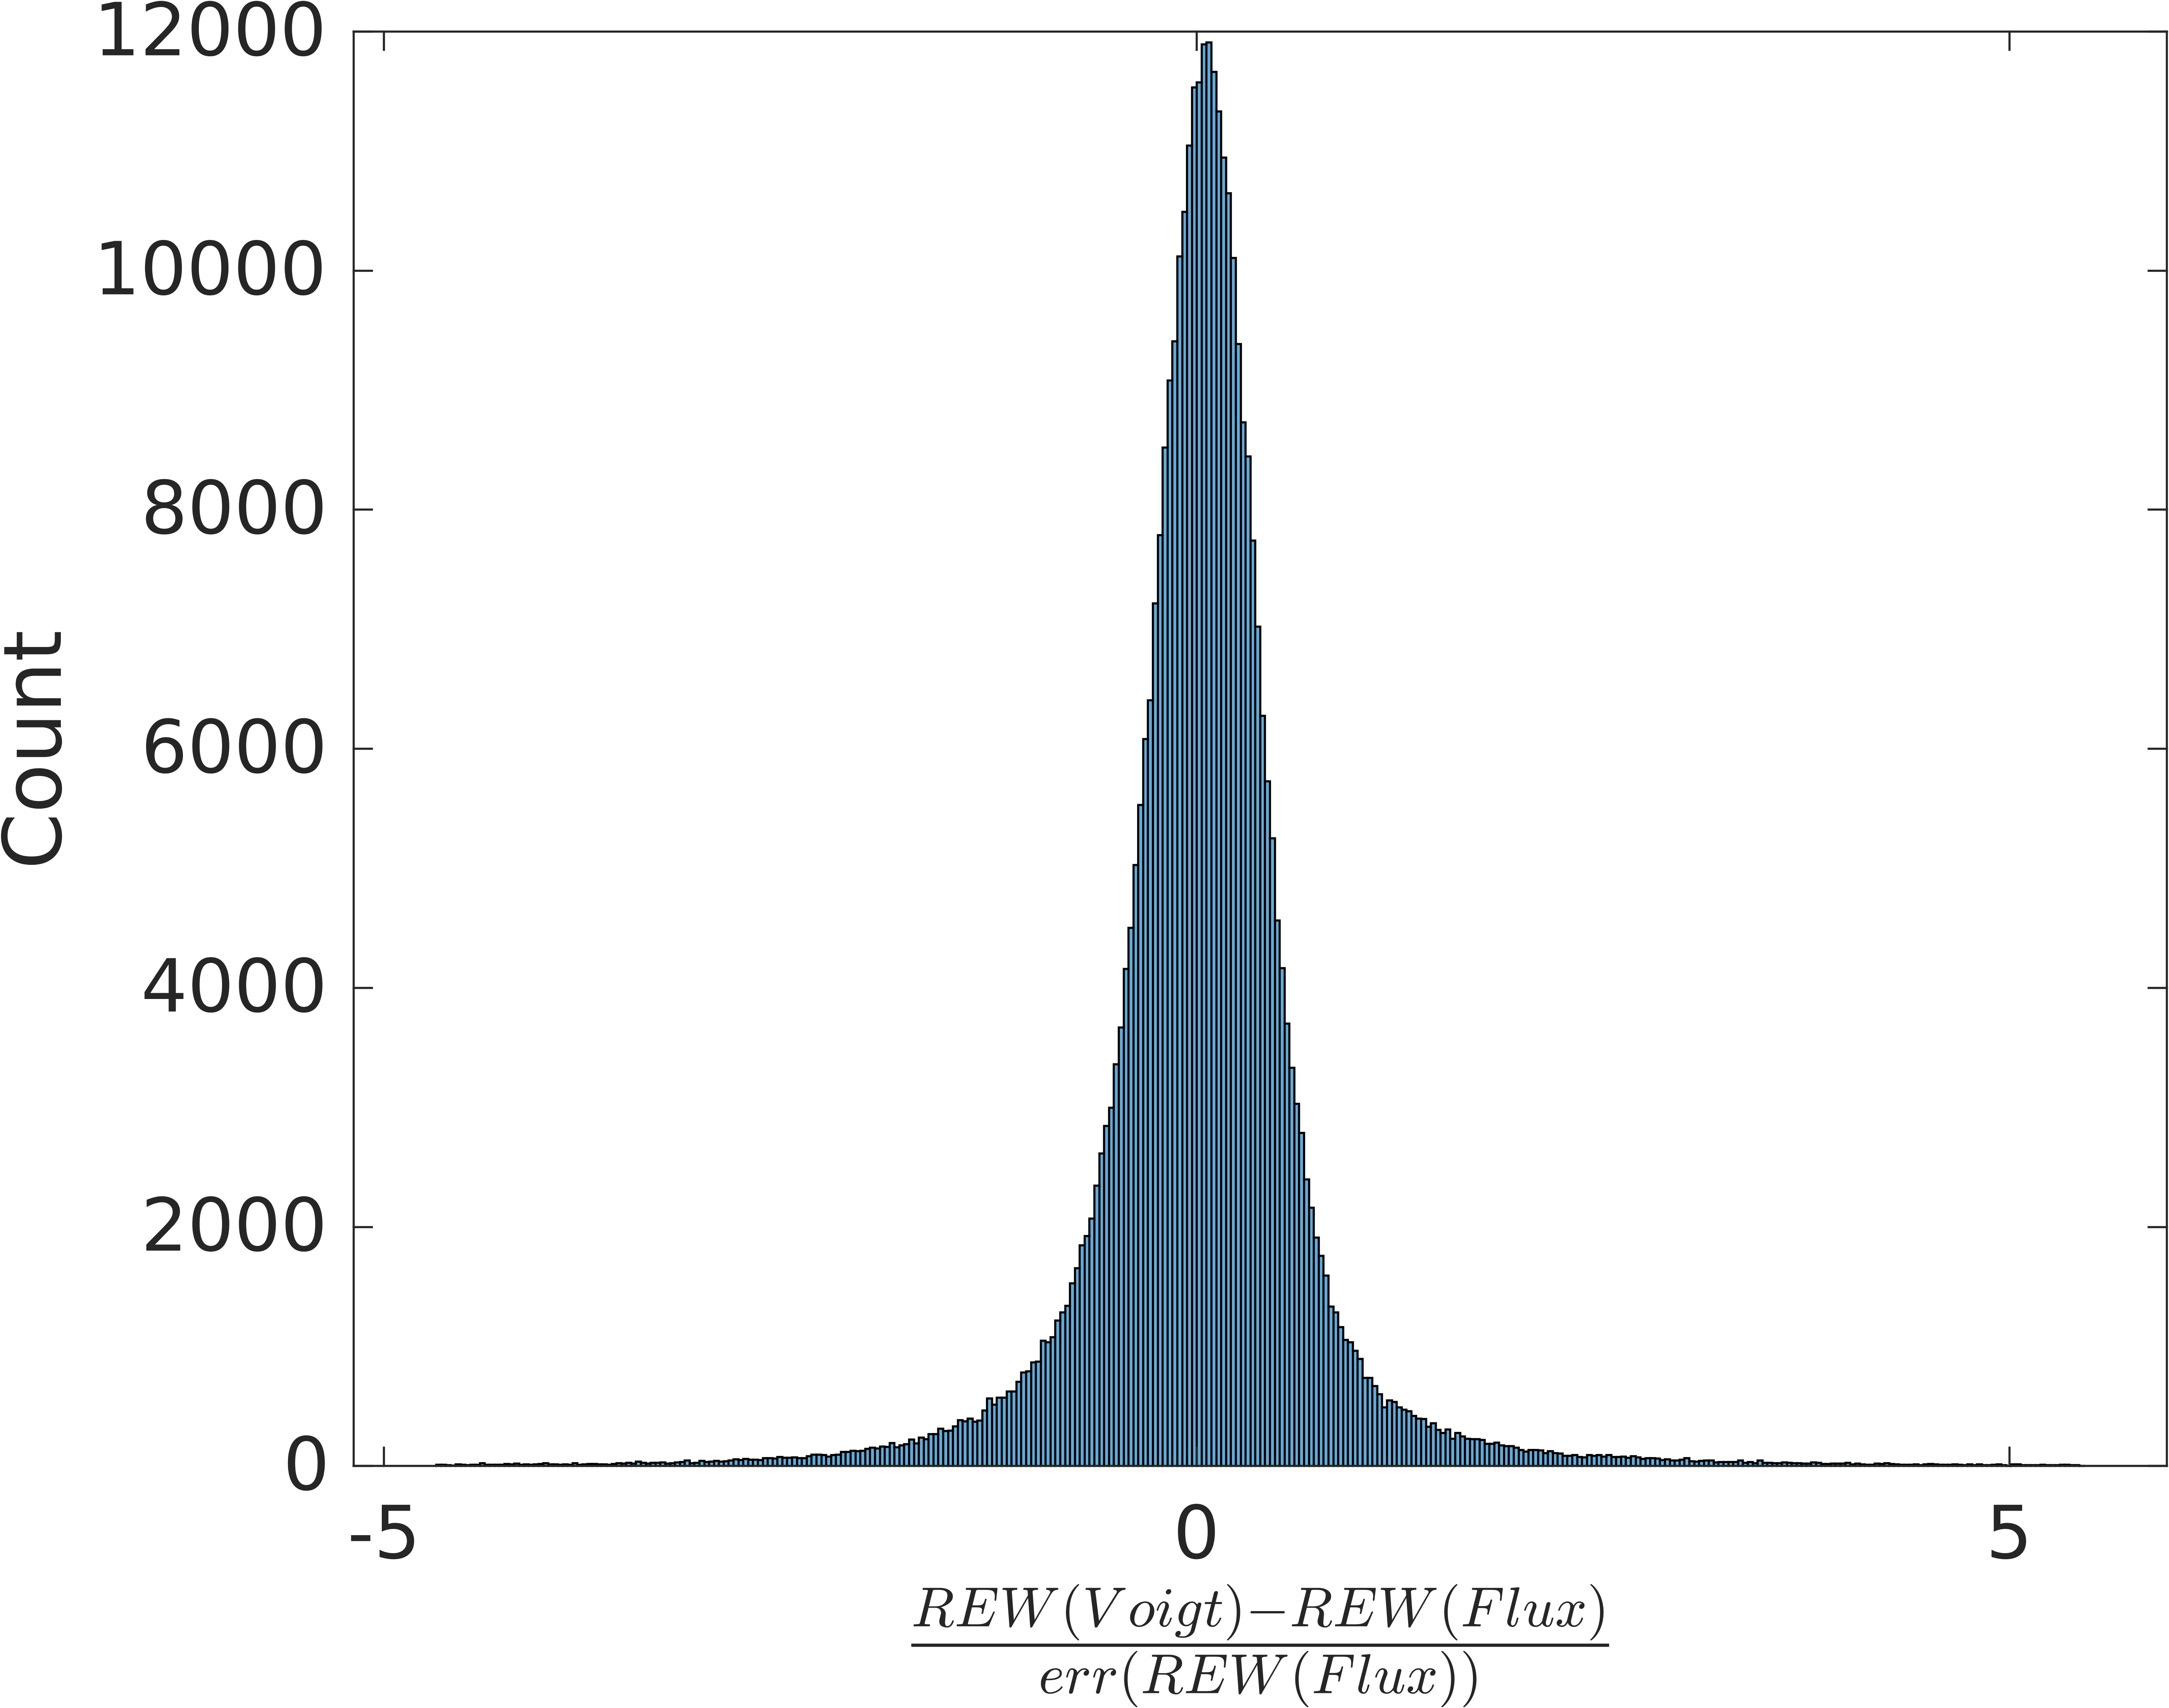
\includegraphics[width=\linewidth]{figs/rREW_1548_voigt_flux_err_SW_2.png}
  \caption{This plot shows that the difference between REW(1548\AA) when we use
  boxcar summation and Voigt profile integration
  is within the estimated error found by flux noise.}
  \label{fig:errDiffREW}
\end{figure}

\begin{table}
  \caption{Table of probabilities (S): first column shows the number of single line absorbers. The 2nd through 4th
   columns   show the number of single~absorbers with probabilities > 65\%, 85\%, and 95\% respectively. } %The last row shows the total number of found absorbers with a certain probability threshold.
  \label{tab:p_L1}
    \begin{tabular}{|l|l|l|l|}
    \hline
    \civ &	$P_n(\model_S)>0.65$ &	$P_n(\model_S)>0.85$&	$P_n(\model_S)>0.95$\\ \hline
    0 &	155905 (84.0\%) &	162533 (87.6\%) &	166675 (89.9\%)\\
    1	& 25441	(13.7\%) & 19159	(10.3\%) & 15366 (8.3\%)\\
    2	& 3210 (1.7\%) &	2914 (1.6\%)	& 2626 (1.4\%)\\
    3	& 675	(0.4\%) & 637 (0.3\%) &	583 (0.3\%)\\
    4 &	161 (0.09\%) &	152 (0.08\%) &	147 (0.08\%)\\
    5	& 29 (0.02\%)	& 26	(0.01\%) & 24 (0.01\%)\\
    6 &	4	(0.00\%) & 4 (0.00\%) &	4 (0.00\%)\\
    % 7 & 0 (0.00\%) & 0 (0.00\%) & 0 (0.00\%)\\
    % Total & 165750 & 136736 &	116228
      \end{tabular}
\end{table}

\begin{figure}
  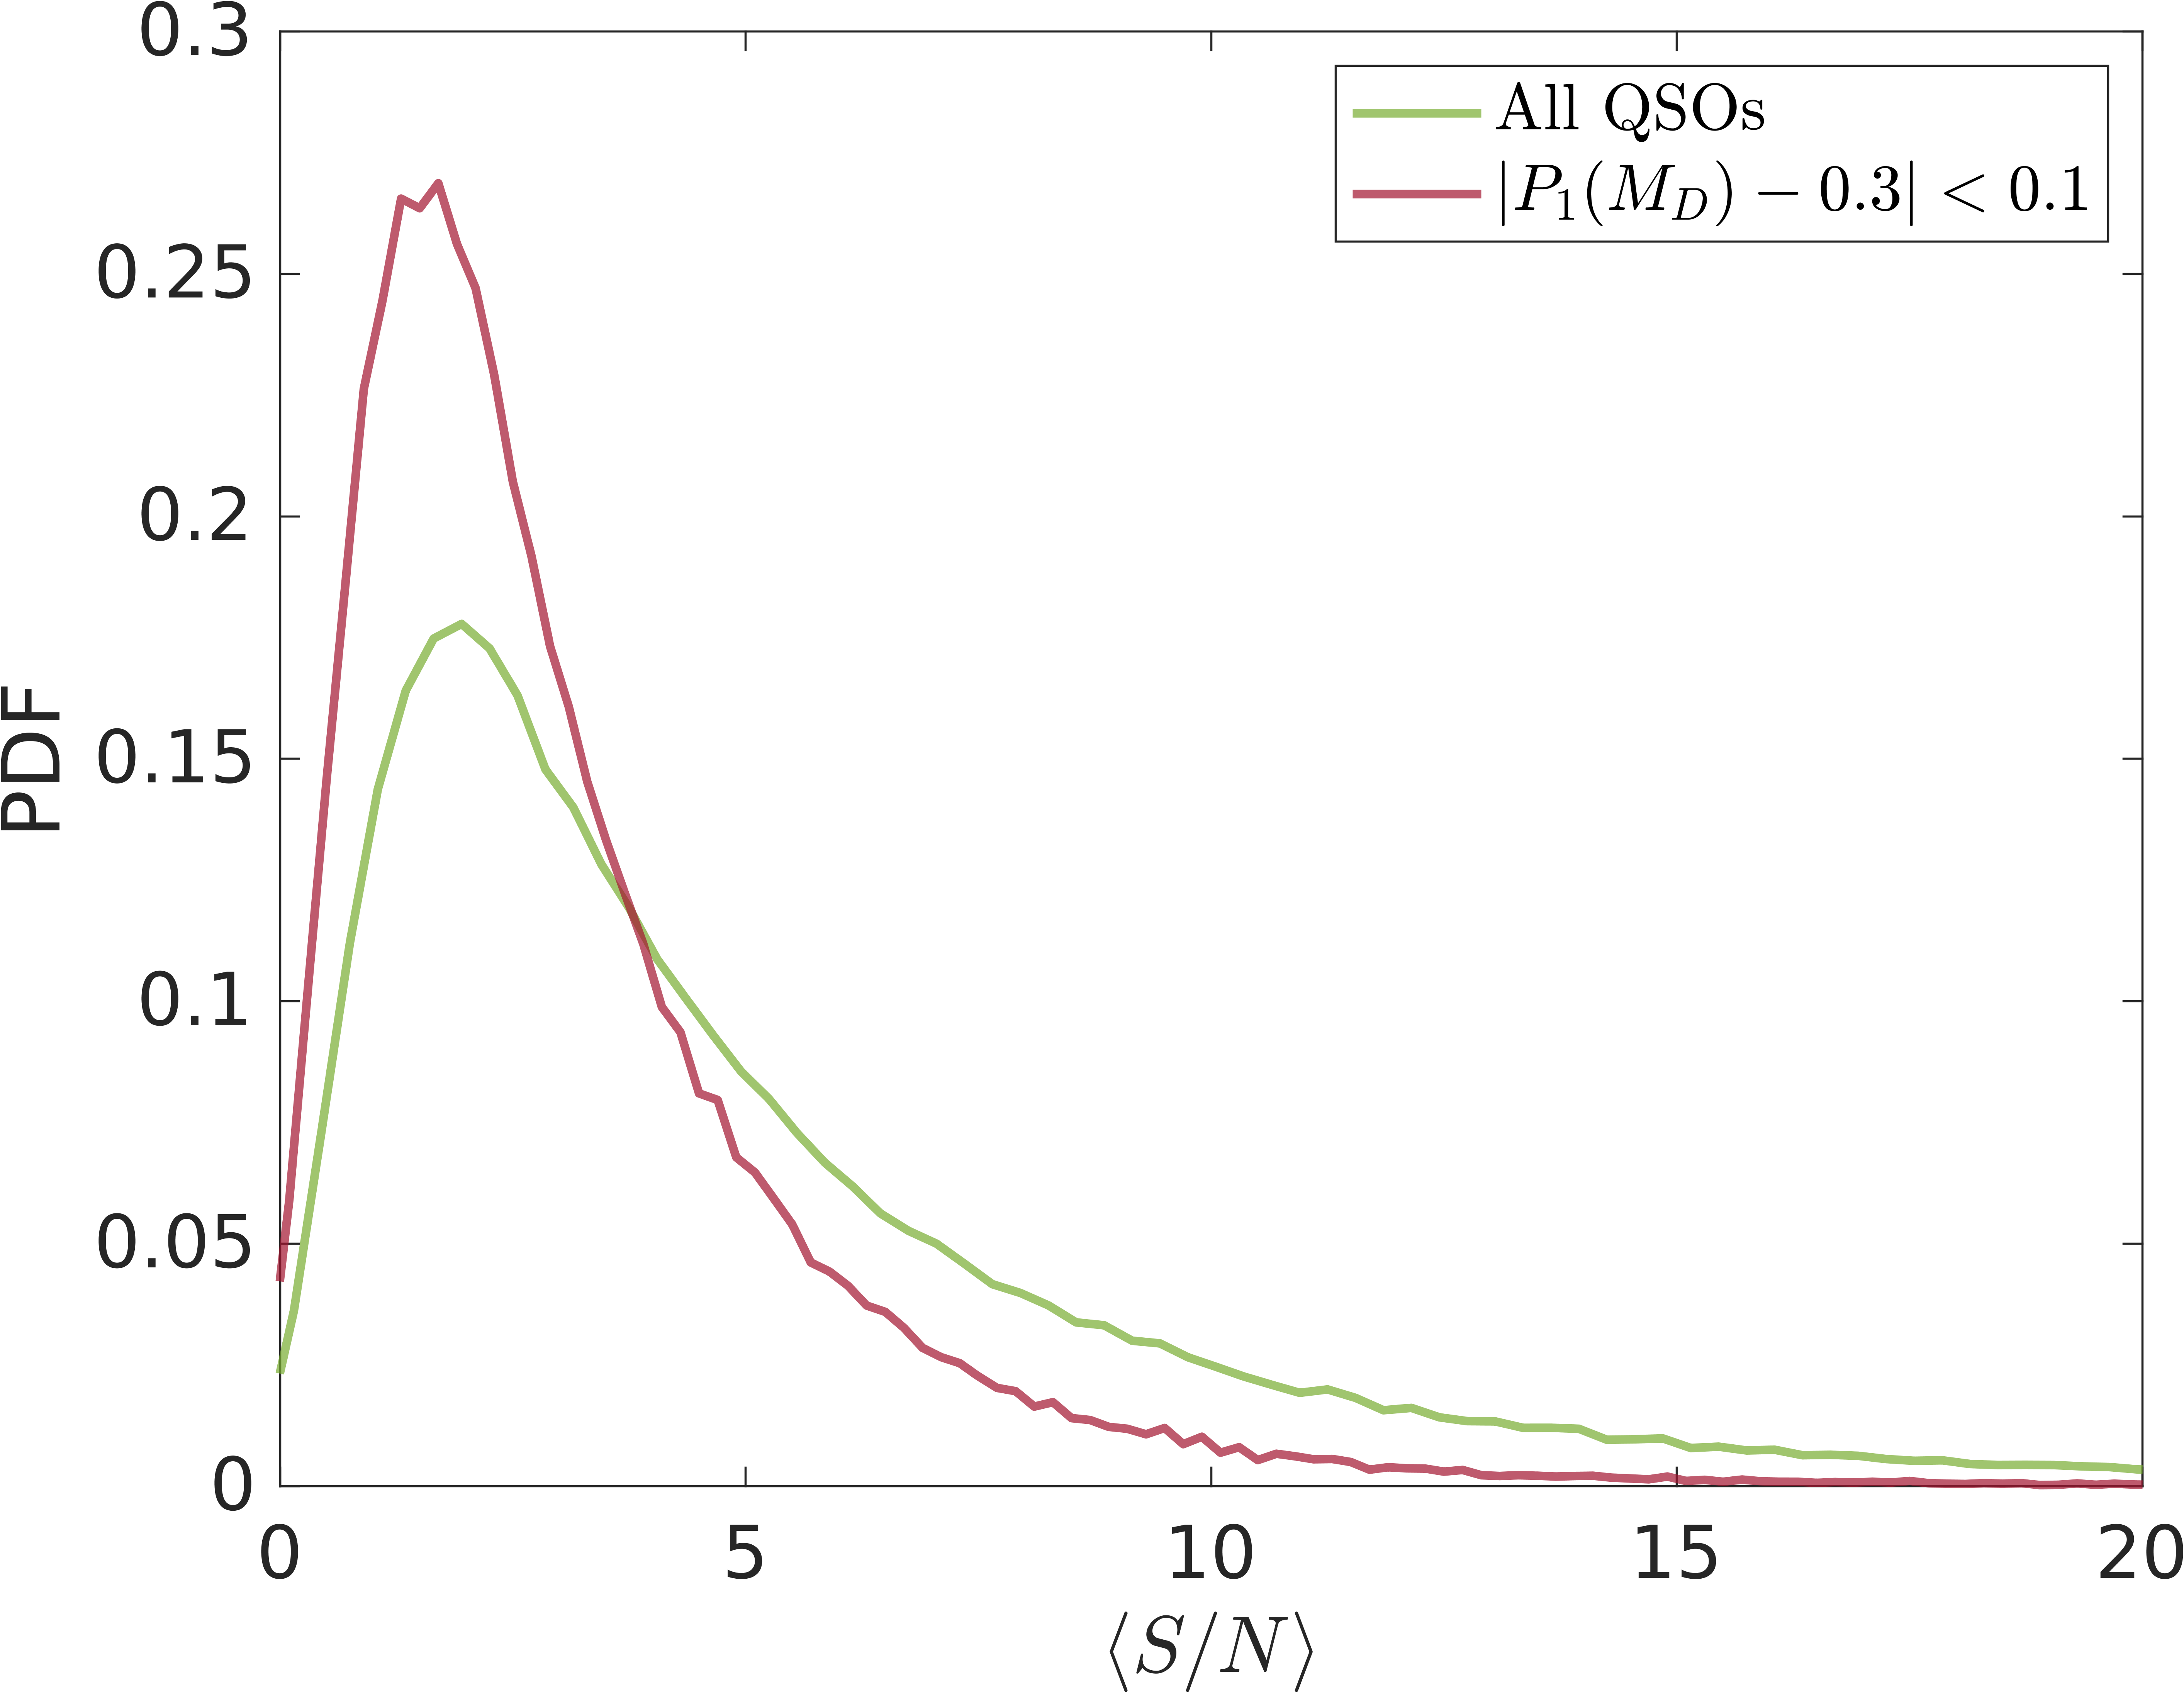
\includegraphics[width=\linewidth]{figs/hist_pc4_mSN_30.png}
\caption{Signal to noise ratio of the ambiguous absorbers found in the first search is systematically lower than
the S/N for all of the searched systems.}
\label{fig:mSNpc4}
\end{figure}

\begin{figure}
  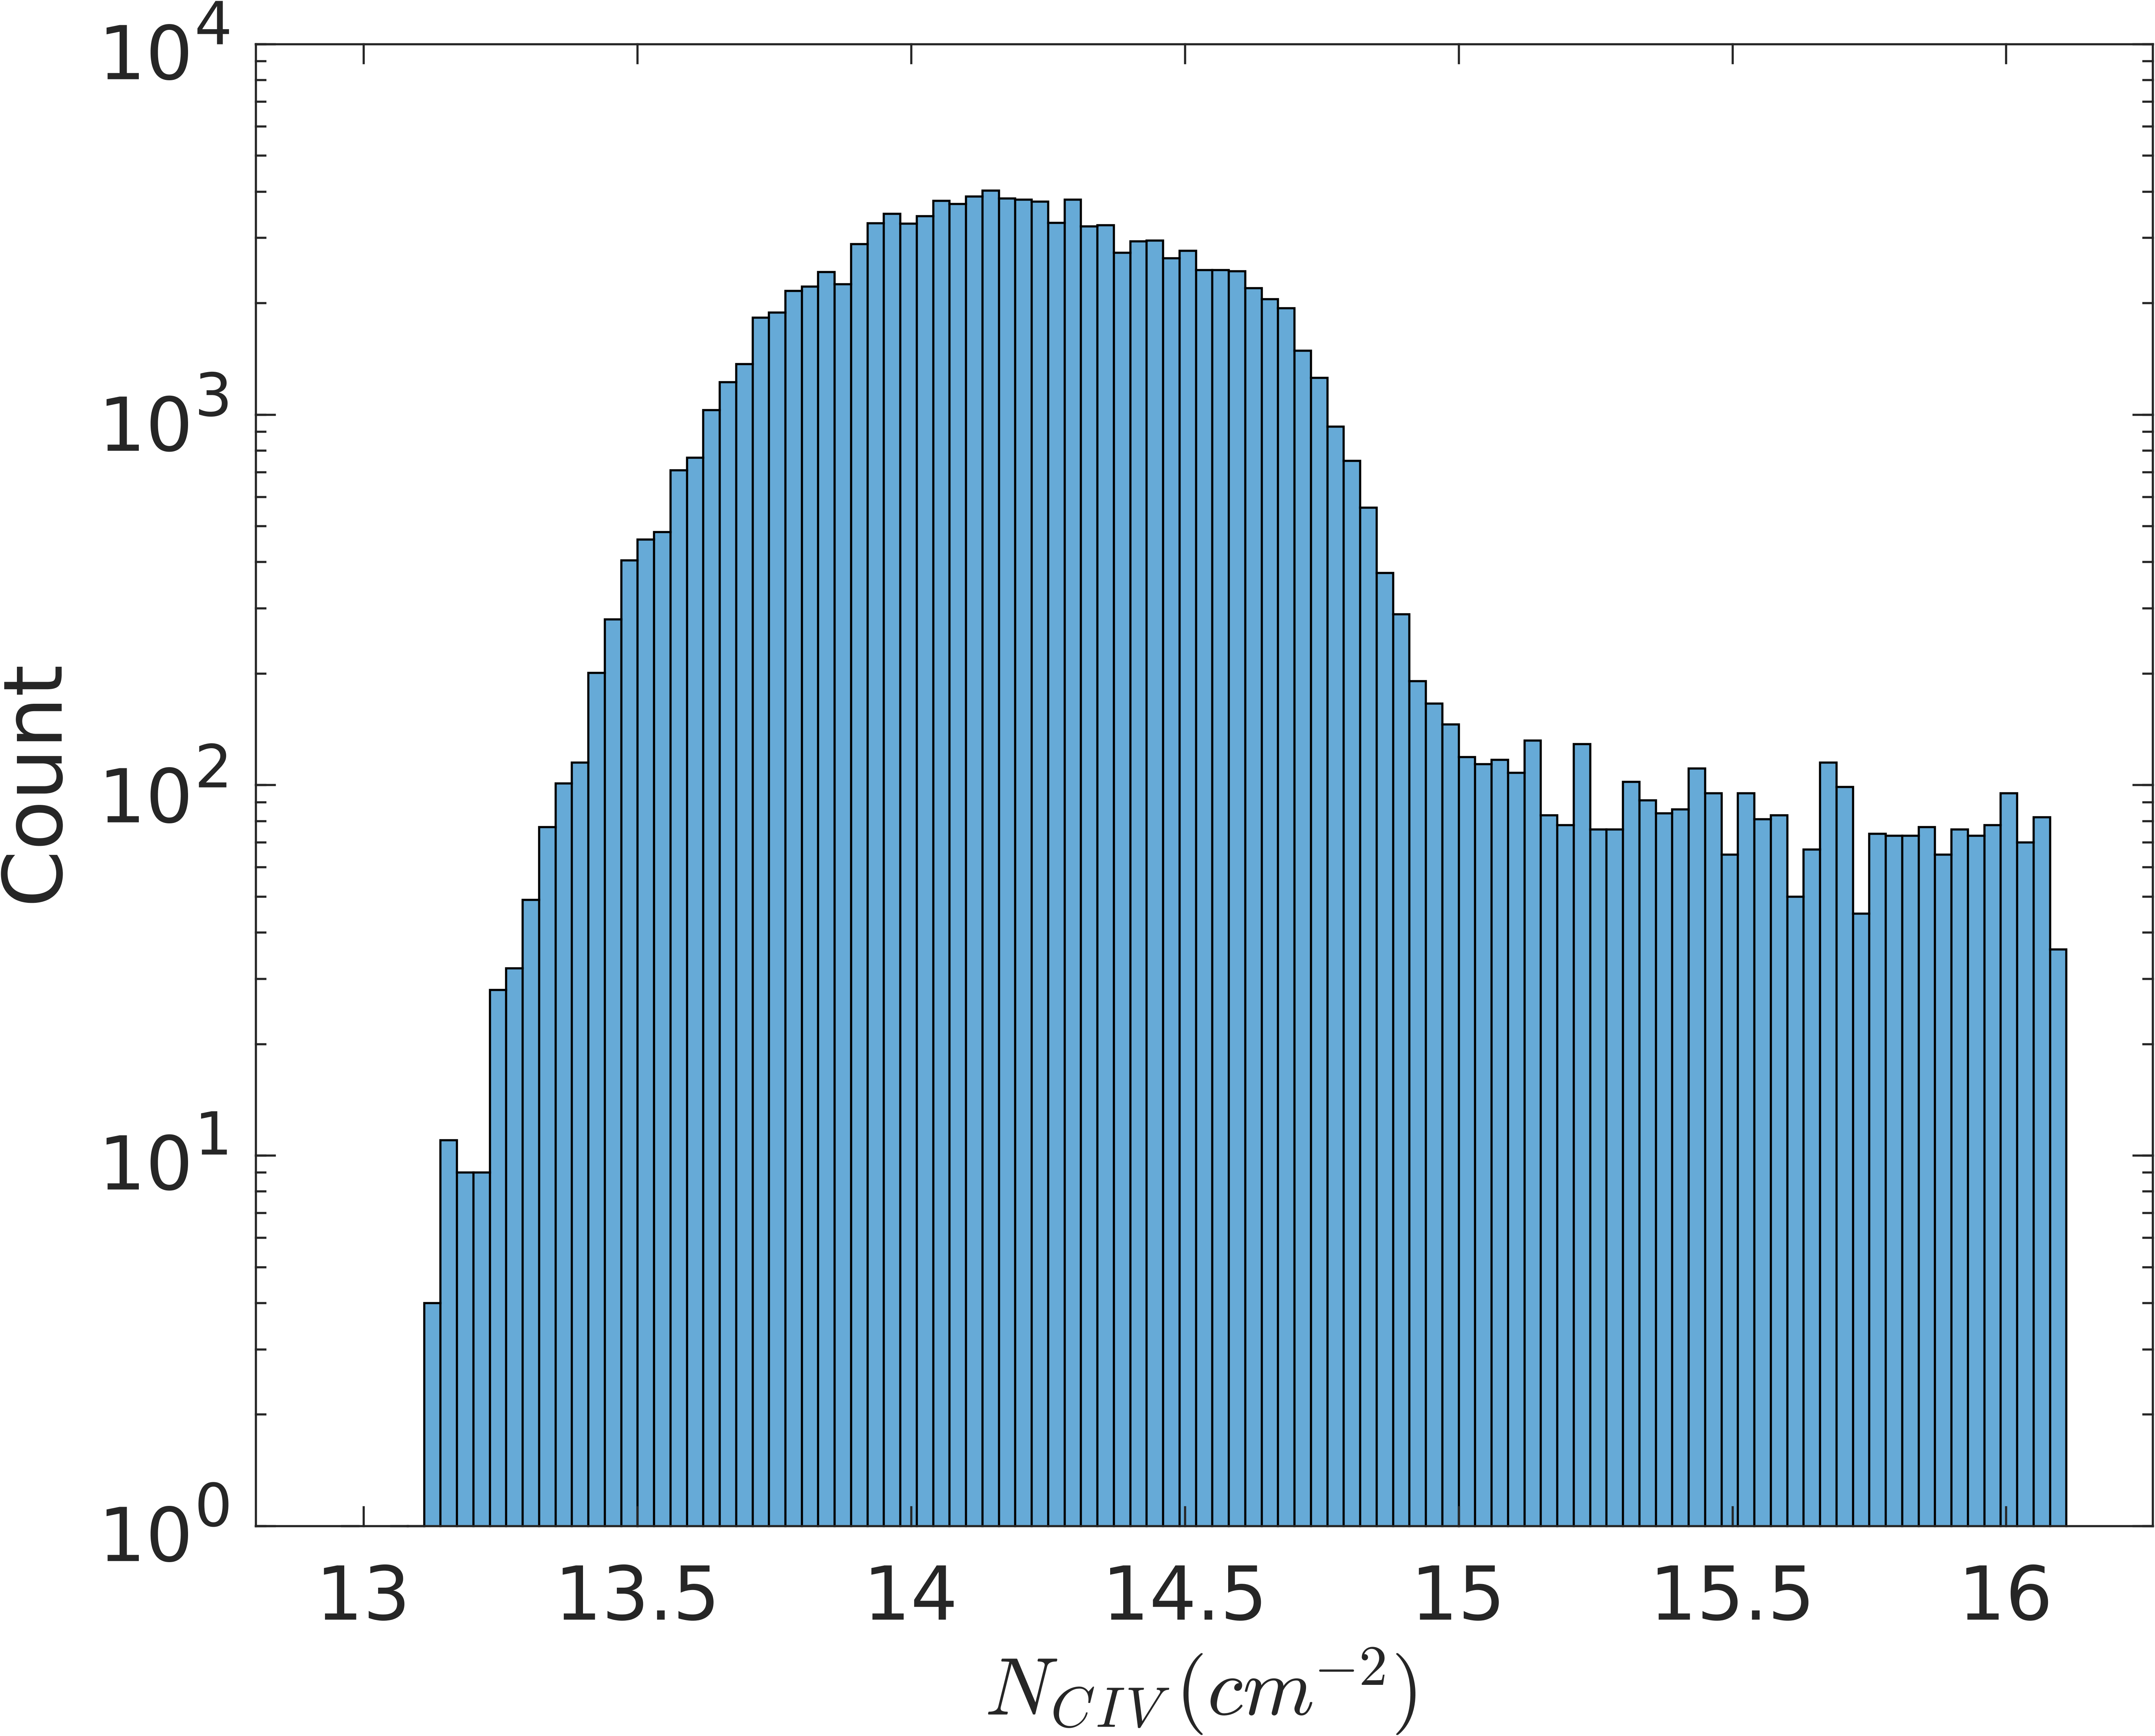
\includegraphics[width=\linewidth]{figs/histDR12_NP95.png}
  \caption{Distribution of the maximum a posterior values for all
  searched column densities in SDSS DR12 spectra with
  $P_n{\model_D}>0.95$}
  \label{fig:DR12N}
\end{figure}


\begin{figure}
  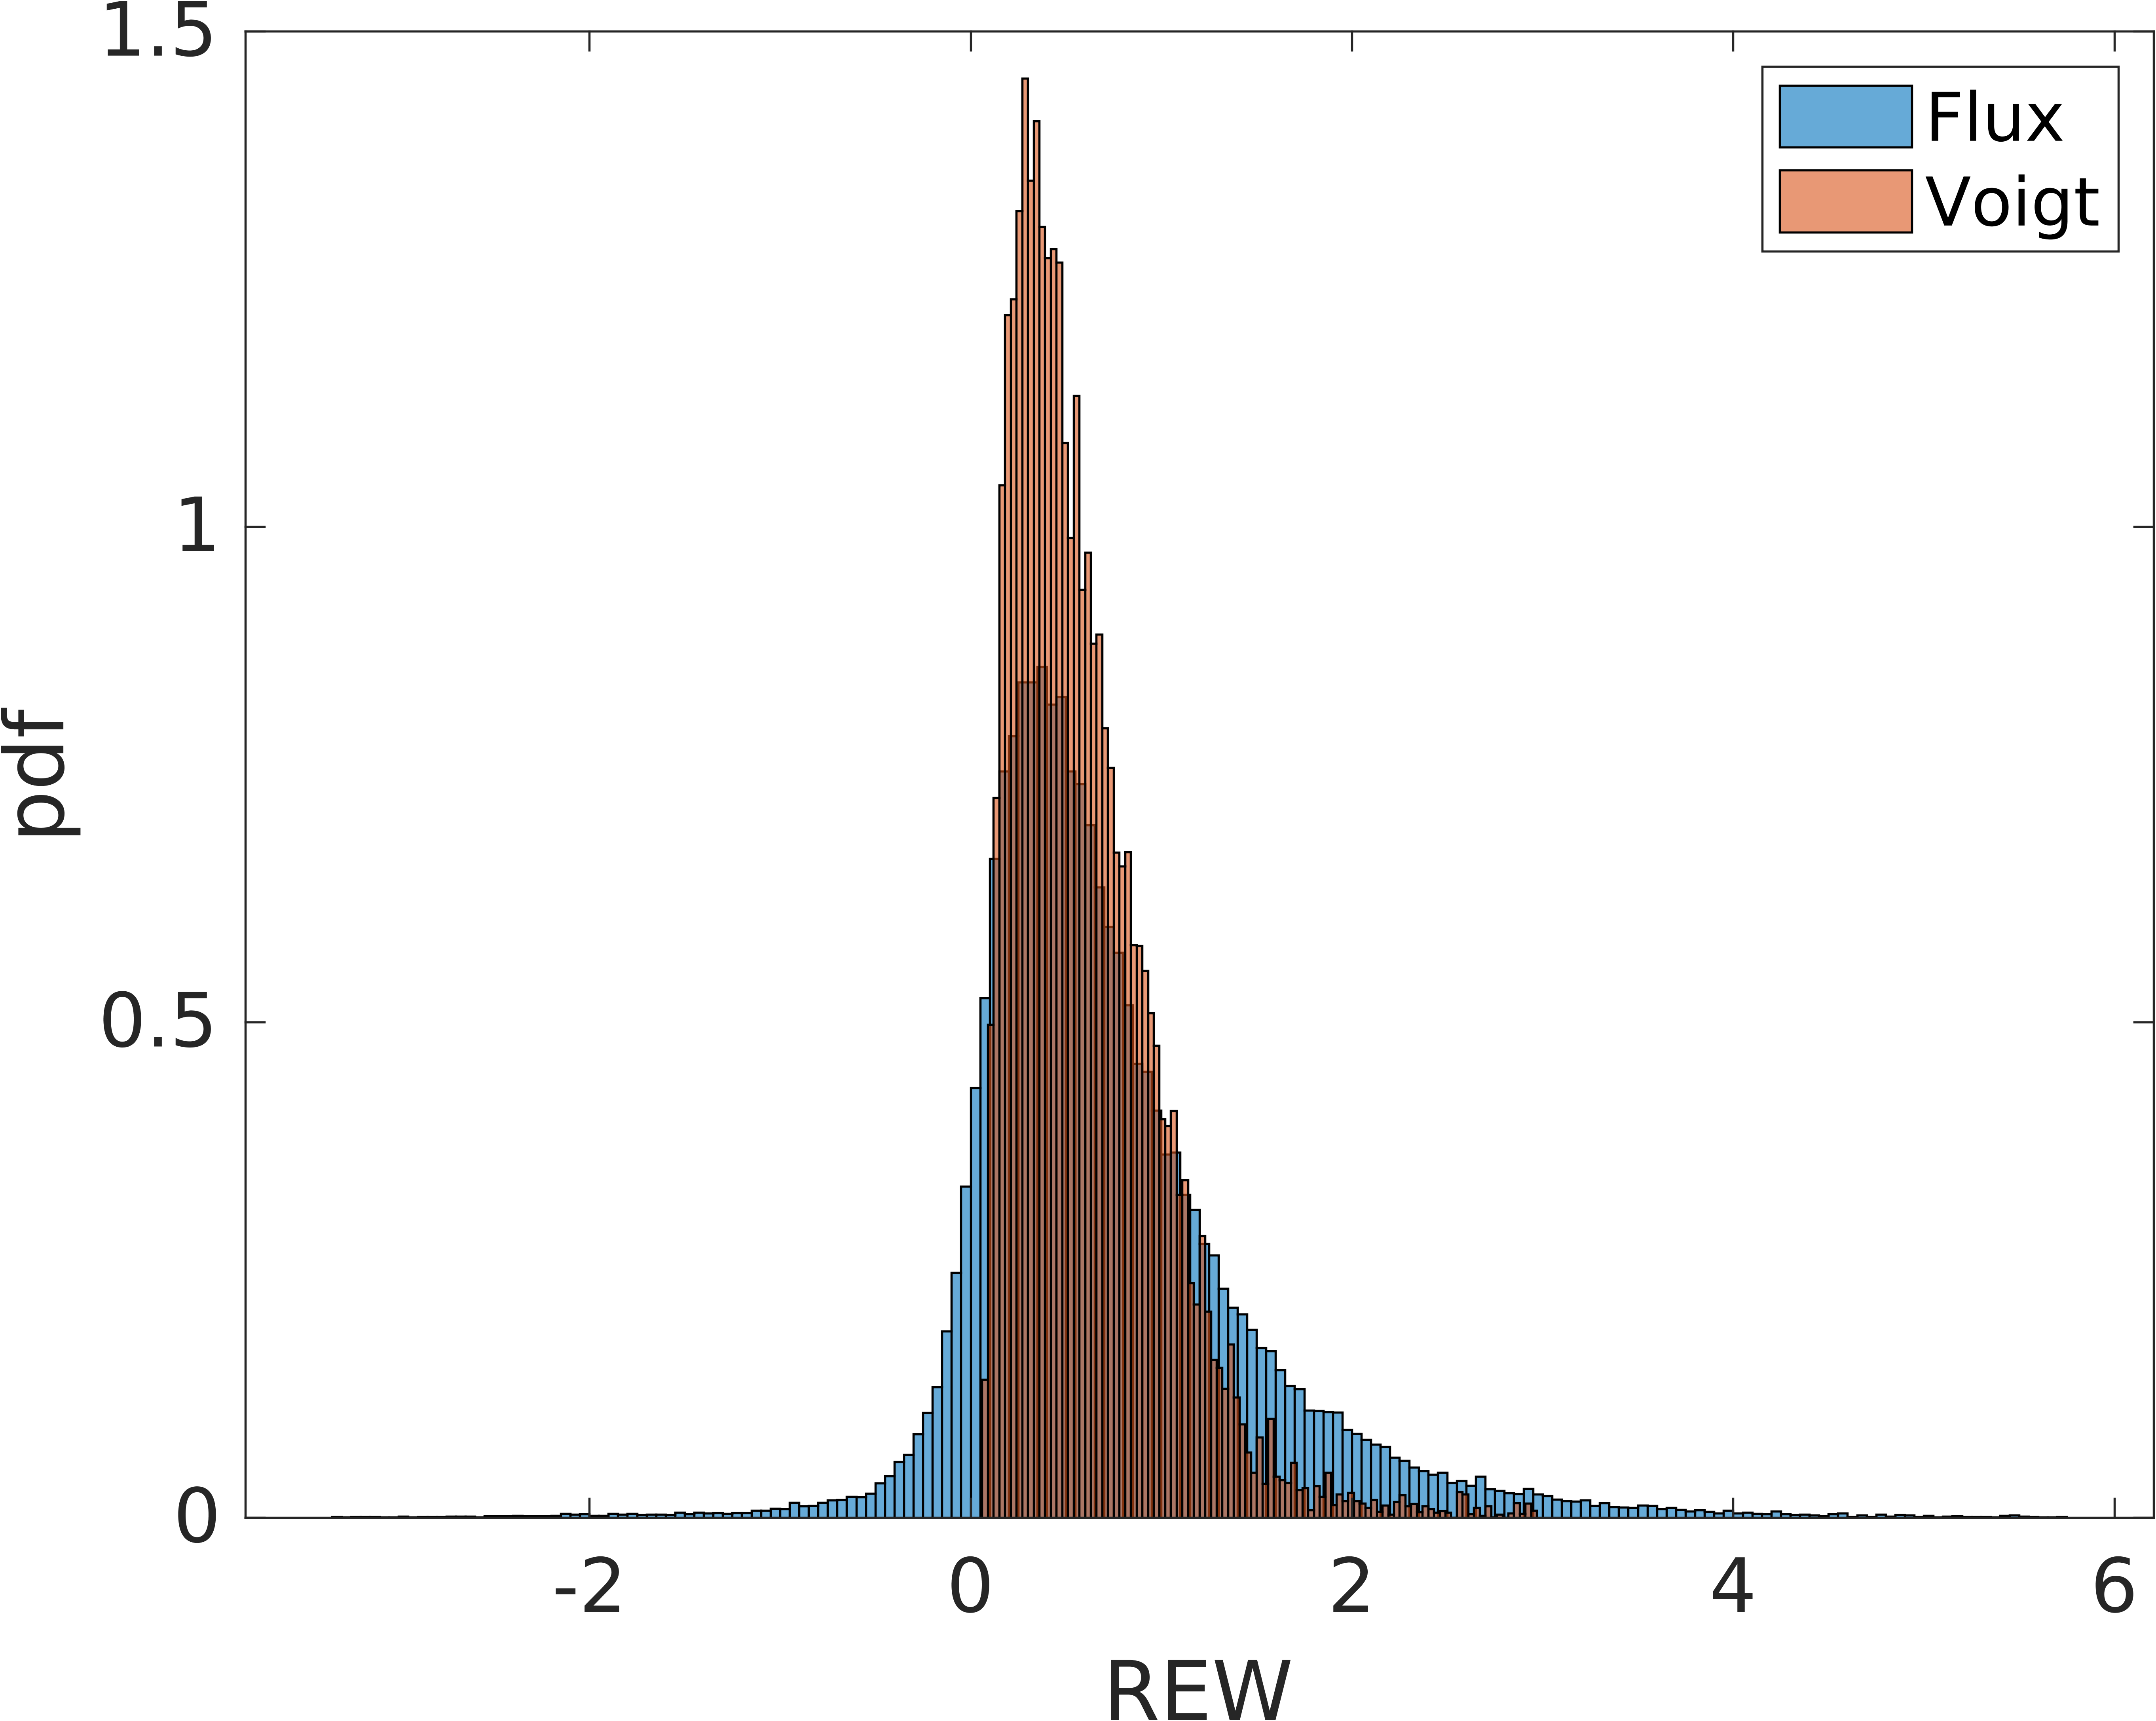
\includegraphics[width=\linewidth]{figs/REW.png}
  \caption{The difference between rest equivalent width of 1548\AA\ in DR12, $\Delta(RWE)$,
  when we integrate the absorption profile resulted from our parameter estimation
  and when we integrate the flux pixels (Eq. \ref{eq:rew_flux})}
  \label{fig:DZdr12}
\end{figure}


\begin{figure}
  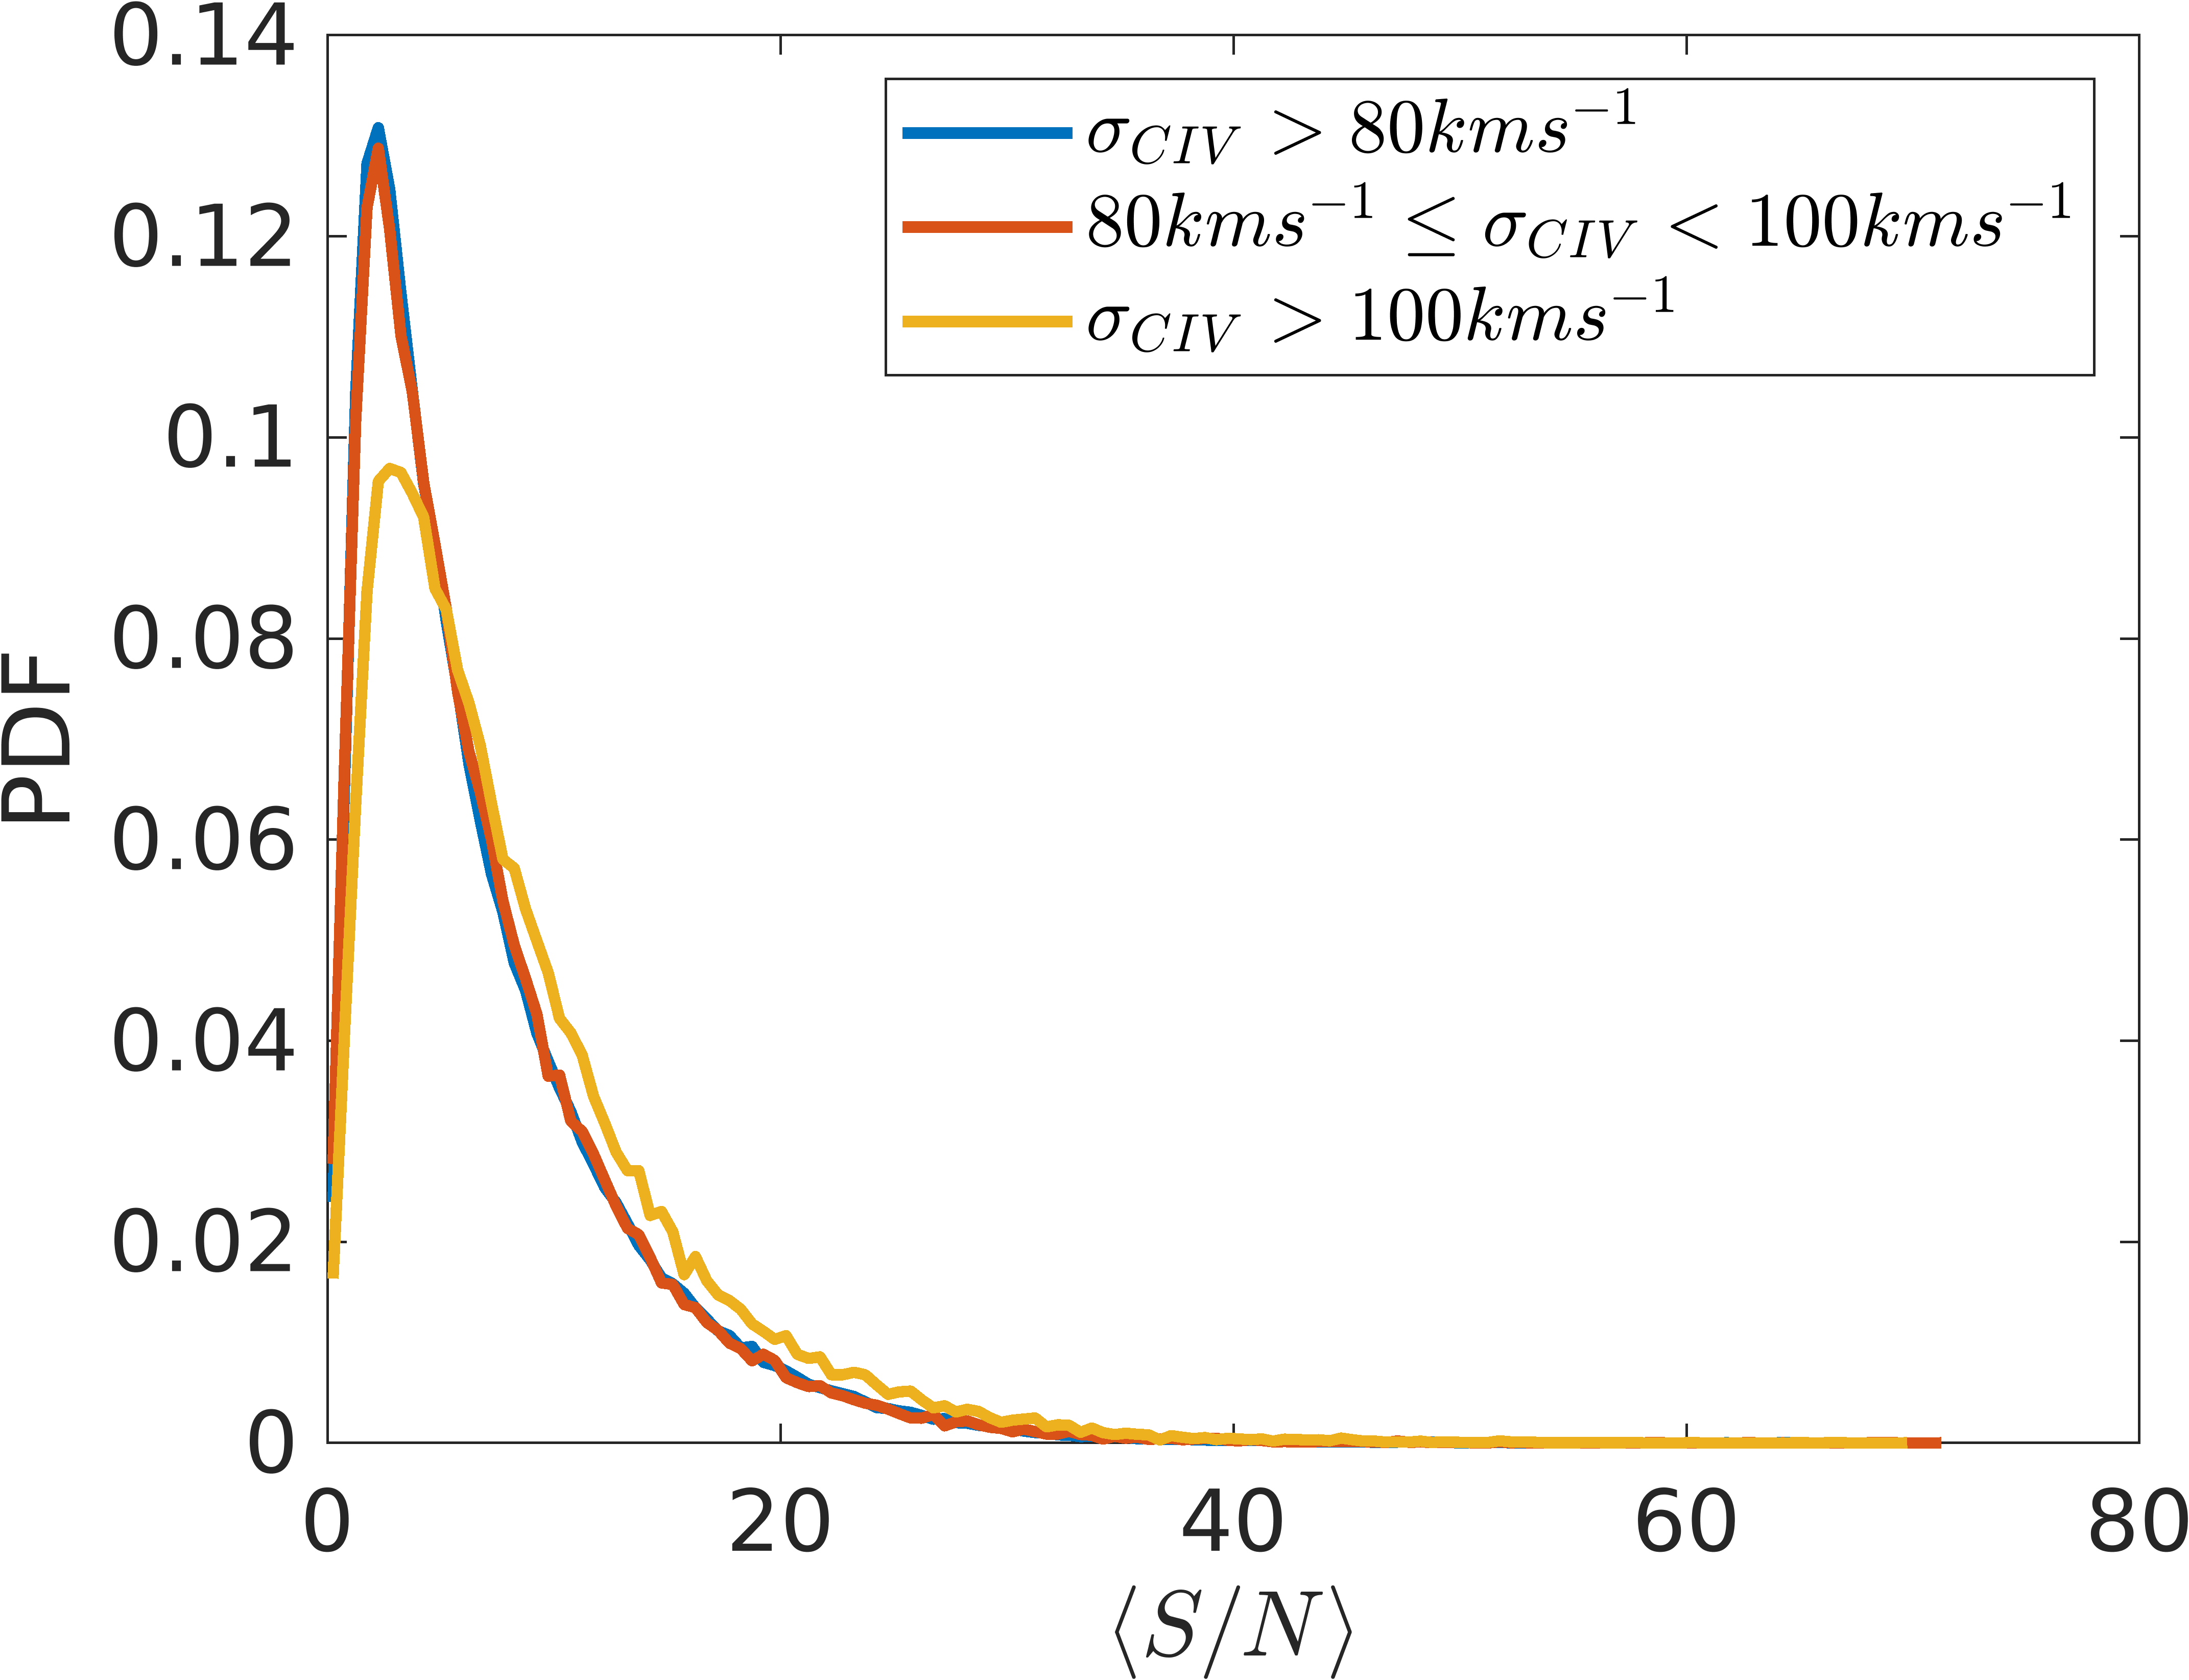
\includegraphics[width=\linewidth]{figs/hist_sigmaCIV_mSN.png}
  \caption{The distribution of average S/N around 5$\sciv$ of the \civ\ doublet for high and
  low $\sciv$ values. High sigma values are not low S/N. }
  \label{fig:mSN-sgima}
\end{figure}

\end{document}


% End of mnras_template.tex